% one dimension
\begin{figure}
	\centering
	\begin{subfigure}{0.34\textwidth}
		\centering
		% This file was created with tikzplotlib v0.10.1.
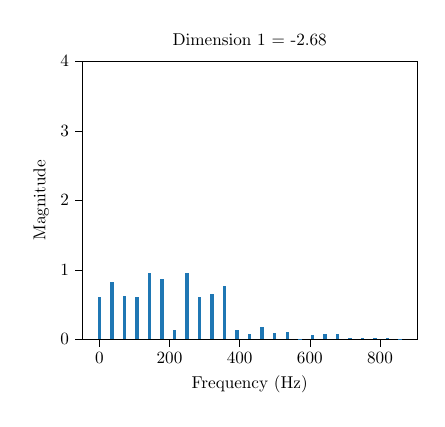
\begin{tikzpicture}[scale=0.62]

\definecolor{darkgray176}{RGB}{176,176,176}
\definecolor{steelblue31119180}{RGB}{31,119,180}

\begin{axis}[
tick align=outside,
tick pos=left,
x grid style={darkgray176},
xlabel={Frequency (Hz)},
xmin=-48.3571428571429, xmax=905.5,
xtick style={color=black},
y grid style={darkgray176},
ylabel={Magnitude},
ymin=0, ymax=4,
title={Dimension 1 = -2.68},
ytick style={color=black}
]
\draw[draw=none,fill=steelblue31119180] (axis cs:-5,0) rectangle (axis cs:5,0.605088098905981);
\draw[draw=none,fill=steelblue31119180] (axis cs:30.7142857142857,0) rectangle (axis cs:40.7142857142857,0.824946037495217);
\draw[draw=none,fill=steelblue31119180] (axis cs:66.4285714285714,0) rectangle (axis cs:76.4285714285714,0.618337924452538);
\draw[draw=none,fill=steelblue31119180] (axis cs:102.142857142857,0) rectangle (axis cs:112.142857142857,0.606547406467815);
\draw[draw=none,fill=steelblue31119180] (axis cs:137.857142857143,0) rectangle (axis cs:147.857142857143,0.952736687378679);
\draw[draw=none,fill=steelblue31119180] (axis cs:173.571428571429,0) rectangle (axis cs:183.571428571429,0.867459344161617);
\draw[draw=none,fill=steelblue31119180] (axis cs:209.285714285714,0) rectangle (axis cs:219.285714285714,0.142171590262196);
\draw[draw=none,fill=steelblue31119180] (axis cs:245,0) rectangle (axis cs:255,0.959357311317153);
\draw[draw=none,fill=steelblue31119180] (axis cs:280.714285714286,0) rectangle (axis cs:290.714285714286,0.614147542320182);
\draw[draw=none,fill=steelblue31119180] (axis cs:316.428571428571,0) rectangle (axis cs:326.428571428571,0.651510920840633);
\draw[draw=none,fill=steelblue31119180] (axis cs:352.142857142857,0) rectangle (axis cs:362.142857142857,0.767848611698322);
\draw[draw=none,fill=steelblue31119180] (axis cs:387.857142857143,0) rectangle (axis cs:397.857142857143,0.130737421425031);
\draw[draw=none,fill=steelblue31119180] (axis cs:423.571428571429,0) rectangle (axis cs:433.571428571429,0.0781024768115382);
\draw[draw=none,fill=steelblue31119180] (axis cs:459.285714285714,0) rectangle (axis cs:469.285714285714,0.174989028847861);
\draw[draw=none,fill=steelblue31119180] (axis cs:495,0) rectangle (axis cs:505,0.0957224281064073);
\draw[draw=none,fill=steelblue31119180] (axis cs:530.714285714286,0) rectangle (axis cs:540.714285714286,0.105812453640171);
\draw[draw=none,fill=steelblue31119180] (axis cs:566.428571428571,0) rectangle (axis cs:576.428571428571,0.00668246230492007);
\draw[draw=none,fill=steelblue31119180] (axis cs:602.142857142857,0) rectangle (axis cs:612.142857142857,0.0584750394429784);
\draw[draw=none,fill=steelblue31119180] (axis cs:637.857142857143,0) rectangle (axis cs:647.857142857143,0.0829703251371982);
\draw[draw=none,fill=steelblue31119180] (axis cs:673.571428571429,0) rectangle (axis cs:683.571428571429,0.0786316144734407);
\draw[draw=none,fill=steelblue31119180] (axis cs:709.285714285714,0) rectangle (axis cs:719.285714285714,0.0183265263662661);
\draw[draw=none,fill=steelblue31119180] (axis cs:745,0) rectangle (axis cs:755,0.0136594016374186);
\draw[draw=none,fill=steelblue31119180] (axis cs:780.714285714286,0) rectangle (axis cs:790.714285714286,0.0150421133154433);
\draw[draw=none,fill=steelblue31119180] (axis cs:816.428571428571,0) rectangle (axis cs:826.428571428571,0.0199113615327003);
\draw[draw=none,fill=steelblue31119180] (axis cs:852.142857142857,0) rectangle (axis cs:862.142857142857,0.00824199961136327);
\end{axis}

\end{tikzpicture}

	\end{subfigure}\hfill
	\begin{subfigure}{0.3\textwidth}
		\centering
		% This file was created with tikzplotlib v0.10.1.
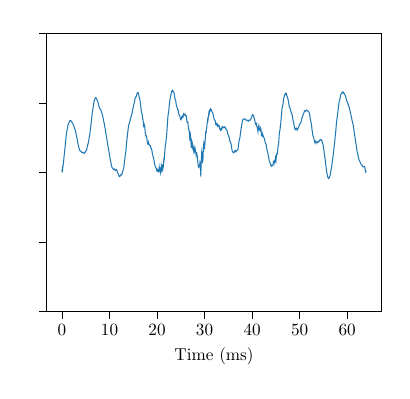
\begin{tikzpicture}[scale=0.62]

\definecolor{darkgray176}{RGB}{176,176,176}
\definecolor{steelblue31119180}{RGB}{31,119,180}

\begin{axis}[
yticklabel={\empty},
tick align=outside,
tick pos=left,
x grid style={darkgray176},
xlabel={Time (ms)},
xmin=-3.2, xmax=67.2,
xtick style={color=black},
y grid style={darkgray176},
% ylabel={Amplitude},
% ymin=-0.15, ymax=0.15,
ymin=-0.1, ymax=0.1,
ytick style={color=black}
]
\addplot [semithick, steelblue31119180]
table {%
0 0
0.0625610948191593 0.00267421979664707
0.125122189638319 0.00195263445792485
0.187683284457478 0.00448575329658223
0.250244379276637 0.00506307051416017
0.312805474095797 0.00741872769886972
0.375366568914956 0.00896099196129705
0.437927663734115 0.0115803680341702
0.500488758553275 0.0133900876509304
0.563049853372434 0.0151754755341063
0.625610948191593 0.0175304286389494
0.688172043010753 0.0195827149455586
0.750733137829912 0.0220035516719752
0.813294232649071 0.0241572310672827
0.875855327468231 0.0260075675241671
0.93841642228739 0.0276190532682753
1.00097751710655 0.029011056083869
1.06353861192571 0.0303319803605681
1.12609970674487 0.0314772311226626
1.18866080156403 0.0323503866813574
1.25122189638319 0.0340090383259345
1.31378299120235 0.0342868589673224
1.37634408602151 0.034962264941104
1.43890518084066 0.0355454103753539
1.50146627565982 0.0360117456070052
1.56402737047898 0.0365307936963797
1.62658846529814 0.0370469956639663
1.6891495601173 0.0372855405697375
1.75171065493646 0.0373638160362883
1.81427174975562 0.0371841114243804
1.87683284457478 0.0371509336557818
1.93939393939394 0.0367688526484099
2.0019550342131 0.0364753106155616
2.06451612903226 0.0361838696464416
2.12707722385142 0.0359691435804378
2.18963831867058 0.0355138606187011
2.25219941348974 0.0352915312351981
2.3147605083089 0.0347998261102134
2.37732160312805 0.0344101194336005
2.43988269794721 0.0336631536920749
2.50244379276637 0.0331262272681571
2.56500488758553 0.0324098647864333
2.62756598240469 0.0318902237095004
2.69012707722385 0.0313611501975318
2.75268817204301 0.030779401080743
2.81524926686217 0.0301372612829257
2.87781036168133 0.0291732079745475
2.94037145650049 0.0278471793837386
3.00293255131965 0.026998937900159
3.06549364613881 0.0261555616457092
3.12805474095797 0.0251639858926059
3.19061583577713 0.0240808387786762
3.25317693059629 0.0226956488526374
3.31573802541544 0.0215881998074457
3.3782991202346 0.0205637725818454
3.44086021505376 0.0194245896512462
3.50342130987292 0.0185915641158907
3.56598240469208 0.0176511272853595
3.62854349951124 0.016837186412203
3.6911045943304 0.0160462343054783
3.75366568914956 0.0156823699676658
3.81622678396872 0.0154439510553638
3.87878787878788 0.0154666042124683
3.94134897360704 0.0152564826052734
4.0039100684262 0.0150434925245487
4.06647116324536 0.01496300729445
4.12903225806452 0.0145273268102638
4.19159335288368 0.0143023412947781
4.25415444770283 0.0141885221670887
4.31671554252199 0.0143579145090496
4.37927663734115 0.0143627272509148
4.44183773216031 0.0143107777445023
4.50439882697947 0.0143003093455631
4.56695992179863 0.0140994674365017
4.62952101661779 0.0139923333422529
4.69208211143695 0.0136977836183788
4.75464320625611 0.013858715826072
4.81720430107527 0.0140708540115626
4.87976539589443 0.0146523808071778
4.94232649071359 0.0149836221114456
5.00488758553275 0.0151687482169821
5.06744868035191 0.0155991362598984
5.13000977517107 0.0159412591371281
5.19257086999022 0.0162529259035227
5.25513196480938 0.017360441337539
5.31769305962854 0.0182014699926999
5.3802541544477 0.0193291187581341
5.44281524926686 0.0200854901912625
5.50537634408602 0.0208316617795537
5.56793743890518 0.0217071624084914
5.63049853372434 0.0229126865049698
5.6930596285435 0.0242266035106175
5.75562072336266 0.0256323526474126
5.81818181818182 0.0267178274013779
5.88074291300098 0.0283921178146279
5.94330400782014 0.0298888944198659
6.0058651026393 0.0314556878562634
6.06842619745846 0.0335125506820042
6.13098729227761 0.0353603800185178
6.19354838709677 0.0371862264169801
6.25610948191593 0.0392754322130921
6.31867057673509 0.0411166230822938
6.38123167155425 0.0428521498174699
6.44379276637341 0.0441375720776246
6.50635386119257 0.0457053787929834
6.56891495601173 0.0472871441710904
6.63147605083089 0.048761960190019
6.69403714565005 0.0498478819788201
6.75659824046921 0.050987220705211
6.81915933528837 0.0516526354504121
6.88172043010753 0.052490993072429
6.94428152492669 0.0530063456738275
7.00684261974585 0.0534649434775289
7.069403714565 0.0537074036634038
7.13196480938416 0.0537072170656885
7.19452590420332 0.0535349667596677
7.25708699902248 0.0530148078673833
7.31964809384164 0.0528068320274003
7.3822091886608 0.0521574912434362
7.44477028347996 0.0515556330096162
7.50733137829912 0.0511457352595857
7.56989247311828 0.0503554332160181
7.63245356793744 0.0496244228928407
7.6950146627566 0.0487227421199297
7.75757575757576 0.0479266882281412
7.82013685239492 0.0471831423031095
7.88269794721408 0.046654381715526
7.94525904203324 0.0460351152001413
8.00782013685239 0.0457550140146898
8.07038123167155 0.0454348212550462
8.13294232649071 0.0452133226112798
8.19550342130987 0.0445972337685198
8.25806451612903 0.0439055550603136
8.32062561094819 0.0433501996252893
8.38318670576735 0.0427576806942476
8.44574780058651 0.0420135908768324
8.50830889540567 0.0413939108542246
8.57086999022483 0.040383708649629
8.63343108504399 0.0394220507029127
8.69599217986315 0.0382373149225439
8.75855327468231 0.0370243414417128
8.82111436950147 0.0361064742824549
8.88367546432062 0.0353182733026156
8.94623655913978 0.034049863776853
9.00879765395894 0.0328304045656122
9.0713587487781 0.0317752120300822
9.13391984359726 0.0303793267955965
9.19648093841642 0.0287503501471361
9.25904203323558 0.0277123870792364
9.32160312805474 0.0264058492072691
9.3841642228739 0.0252075347437624
9.44672531769306 0.0238300412674803
9.50928641251222 0.0225178186025176
9.57184750733138 0.0210519984932589
9.63440860215054 0.0198594470538439
9.6969696969697 0.0187120908363299
9.75953079178886 0.0173988586176962
9.82209188660802 0.0162397695983872
9.88465298142718 0.0150185930283188
9.94721407624633 0.0135728019423499
10.0097751710655 0.0123385272515921
10.0723362658847 0.0110240861762566
10.1348973607038 0.00961095098504398
10.197458455523 0.00825266510554073
10.2600195503421 0.0075971999443259
10.3225806451613 0.00651535481935547
10.3851417399804 0.00549221840684365
10.4477028347996 0.00441473745945787
10.5102639296188 0.00380801213386297
10.5728250244379 0.00333096788884782
10.6353861192571 0.0030224520516448
10.6979472140762 0.00274330640315485
10.7605083088954 0.00251342399357176
10.8230694037146 0.00208306508657695
10.8856304985337 0.00217947526630069
10.9481915933529 0.00227255503649761
11.010752688172 0.00244182444387867
11.0733137829912 0.00224105331533291
11.1358748778104 0.00175680994681599
11.1984359726295 0.00137892175367501
11.2609970674487 0.0013601645838218
11.3235581622678 0.001649708713779
11.386119257087 0.00193779625522951
11.4486803519062 0.00198972274349931
11.5112414467253 0.00166785174057631
11.5738025415445 0.00142994691833548
11.6363636363636 0.00061140903695063
11.6989247311828 -0.000307942650491191
11.761485826002 -0.000503915605132532
11.8240469208211 -0.00113124737401337
11.8866080156403 -0.00155196709236092
11.9491691104594 -0.00214502619049591
12.0117302052786 -0.00279614021264213
12.0742913000978 -0.00304161296212429
12.1368523949169 -0.00297893156076282
12.1994134897361 -0.00285662688817447
12.2619745845552 -0.00236801814582865
12.3245356793744 -0.0021942504504122
12.3870967741935 -0.00160614665477507
12.4496578690127 -0.00156108215123502
12.5122189638319 -0.0018311939707512
12.574780058651 -0.00173706366869012
12.6373411534702 -0.000912511972519309
12.6999022482893 -0.000196902665836721
12.7624633431085 0.000736978850013351
12.8250244379277 0.00106108622335968
12.8875855327468 0.00214182240806542
12.950146627566 0.00270913908383713
13.0127077223851 0.00340024156829129
13.0752688172043 0.00556807706673299
13.1378299120235 0.00725564627725183
13.2003910068426 0.00904701511400187
13.2629521016618 0.0112418273021399
13.3255131964809 0.0124709883655621
13.3880742913001 0.0139866596431938
13.4506353861193 0.0154722398884398
13.5131964809384 0.0179199806613919
13.5757575757576 0.0204215760935437
13.6383186705767 0.0226809065843607
13.7008797653959 0.0248251628578583
13.7634408602151 0.0266148869789416
13.8260019550342 0.0284216282261082
13.8885630498534 0.0303372205931508
13.9511241446725 0.0320307074273087
14.0136852394917 0.0336226689249627
14.0762463343109 0.0342720239436871
14.13880742913 0.0349491323751351
14.2013685239492 0.0356921560931241
14.2639296187683 0.0364141654485394
14.3264907135875 0.0373742953598325
14.3890518084066 0.0380467732554394
14.4516129032258 0.0389382684182736
14.514173998045 0.039927060713123
14.5767350928641 0.0404909389459493
14.6392961876833 0.0411950073032872
14.7018572825024 0.0419001485442311
14.7644183773216 0.0429625525753781
14.8269794721408 0.0438603695558488
14.8895405669599 0.0452642597727849
14.9521016617791 0.0463684541105001
15.0146627565982 0.0474161693220002
15.0772238514174 0.0484258940230367
15.1397849462366 0.048982958699907
15.2023460410557 0.0497803344033506
15.2649071358749 0.051131768807594
15.327468230694 0.0521033428106839
15.3900293255132 0.0531876813511083
15.4525904203324 0.0538189128325307
15.5151515151515 0.0541310210458257
15.5777126099707 0.0543522023735158
15.6402737047898 0.0549303894463785
15.702834799609 0.0555825384328267
15.7653958944282 0.0564133933201826
15.8279569892473 0.056831538196533
15.8905180840665 0.0572587951329534
15.9530791788856 0.057280189141937
16.0156402737048 0.0573616571822736
16.0782013685239 0.056989228402065
16.1407624633431 0.0559466459741952
16.2033235581623 0.0549218033787267
16.2658846529814 0.0539930620970876
16.3284457478006 0.0531750289925382
16.3910068426197 0.0521099569871366
16.4535679374389 0.0510703175386026
16.5161290322581 0.0493302415575712
16.5786901270772 0.0474945895286424
16.6412512218964 0.0456468005039213
16.7038123167155 0.0437111058040274
16.7663734115347 0.0426618811835554
16.8289345063539 0.0419866980607908
16.891495601173 0.0413465699197348
16.9540566959922 0.0398208843953798
17.0166177908113 0.0385363369120443
17.0791788856305 0.0372270050723532
17.1417399804497 0.0345423184062117
17.2043010752688 0.032461166021324
17.266862170088 0.0347551361239813
17.3294232649071 0.0341661413175619
17.3919843597263 0.0338865765739134
17.4545454545455 0.0314861332828348
17.5171065493646 0.0286533663273295
17.5796676441838 0.0271085365361307
17.6422287390029 0.0262852582228411
17.7047898338221 0.0263691197621945
17.7673509286412 0.0262591917002219
17.8299120234604 0.0251460206091317
17.8924731182796 0.023419109804015
17.9550342130987 0.0213664465766848
18.0175953079179 0.0208063320833043
18.080156402737 0.0203971048855275
18.1427174975562 0.0208537711262091
18.2052785923754 0.0216071604644536
18.2678396871945 0.020109887729205
18.3304007820137 0.0199684586124686
18.3929618768328 0.0197349161051673
18.455522971652 0.0194785226671752
18.5180840664712 0.0194128193889807
18.5806451612903 0.0193844509701575
18.6432062561095 0.0188214922176341
18.7057673509286 0.0173547650001878
18.7683284457478 0.0172885383187064
18.830889540567 0.0166502374325417
18.8934506353861 0.0162434242228783
18.9560117302053 0.0150629650757722
19.0185728250244 0.013391328265459
19.0811339198436 0.0127082065490683
19.1436950146628 0.0115744774434661
19.2062561094819 0.0109363535085906
19.2688172043011 0.0104743799254779
19.3313782991202 0.00898958691272917
19.3939393939394 0.00790707682344046
19.4565004887586 0.0066469337168502
19.5190615835777 0.00564898771733657
19.5816226783969 0.0047800187185363
19.644183773216 0.00409872611968224
19.7067448680352 0.00366864474681465
19.7693059628544 0.00332232838895314
19.8318670576735 0.00288059430803197
19.8944281524927 0.00273982084238809
19.9569892473118 0.000845879196159301
20.019550342131 0.000760033273321092
20.0821114369501 0.00095205489120001
20.1446725317693 0.0019063416846599
20.2072336265885 0.00162790942926211
20.2697947214076 0.000875847490608168
20.3323558162268 0.000575767573286014
20.3949169110459 0.00160671152786251
20.4574780058651 0.00388647337332149
20.5200391006843 0.00233205468489453
20.5826001955034 0.00152916488540837
20.6451612903226 0.00328123563479993
20.7077223851417 0.00326864568303582
20.7702834799609 -0.00020999720325568
20.8328445747801 0.000763068778598764
20.8954056695992 0.00438050786442945
20.9579667644184 0.0029384327555332
21.0205278592375 0.000206796255760179
21.0830889540567 0.00278985447351359
21.1456500488759 0.00508365880075263
21.208211143695 0.00488976083280753
21.2707722385142 0.00338998097718811
21.3333333333333 0.00464094616472721
21.3958944281525 0.00786668587683582
21.4584555229717 0.0097706981789856
21.5210166177908 0.00937353533384038
21.58357771261 0.0119085969113884
21.6461388074291 0.0154543465107155
21.7086999022483 0.0183054468160238
21.7712609970674 0.0201115640770655
21.8338220918866 0.0206162288205977
21.8963831867058 0.0229037094675551
21.9589442815249 0.0247902948616886
22.0215053763441 0.0266693644826451
22.0840664711632 0.030081022257679
22.1466275659824 0.0328973525659867
22.2091886608016 0.0361175192438088
22.2717497556207 0.0395221697477913
22.3343108504399 0.041304173204731
22.396871945259 0.0427716355006104
22.4594330400782 0.0439727842436333
22.5219941348974 0.04629844911615
22.5845552297165 0.0490542658088494
22.6471163245357 0.0508796651724759
22.7096774193548 0.0520982259223538
22.772238514174 0.0532420461729737
22.8347996089932 0.0545685695609914
22.8973607038123 0.0551733477560044
22.9599217986315 0.0559879976305619
23.0224828934506 0.0578949249723702
23.0850439882698 0.0583804640755101
23.147605083089 0.0584930904439031
23.2101661779081 0.0588970233377648
23.2727272727273 0.0583844416859475
23.3352883675464 0.0586766382225972
23.3978494623656 0.0583387540593263
23.4604105571848 0.0581928974350701
23.5229716520039 0.0575271020438577
23.5855327468231 0.0569285704942742
23.6480938416422 0.0559307399787599
23.7106549364614 0.0543003477199861
23.7732160312805 0.0534002241184198
23.8357771260997 0.0520780251260377
23.8983382209189 0.0516900767864457
23.960899315738 0.0508313895888692
24.0234604105572 0.049175866521742
24.0860215053763 0.0479400197584783
24.1485826001955 0.0473373903895665
24.2111436950147 0.046511578878874
24.2737047898338 0.0462514713264543
24.336265884653 0.0451448697848054
24.3988269794721 0.0451817311991083
24.4613880742913 0.0443530065114023
24.5239491691105 0.0426578202784673
24.5865102639296 0.0416546216196329
24.6490713587488 0.0413088361156389
24.7116324535679 0.041108225174576
24.7741935483871 0.0408650341654016
24.8367546432063 0.0398515648812143
24.8993157380254 0.038847956440447
24.9618768328446 0.0380346358281252
25.0244379276637 0.0378304746854078
25.0869990224829 0.0382387661689188
25.1495601173021 0.0390100164114992
25.2121212121212 0.0399538556283171
25.2746823069404 0.040413034577305
25.3372434017595 0.0400065938966715
25.3998044965787 0.0394734188400843
25.4623655913978 0.0394740778832666
25.524926686217 0.0411028750513918
25.5874877810362 0.0420756560485384
25.6500488758553 0.0417780720757162
25.7126099706745 0.0412677814774324
25.7751710654936 0.041175230032057
25.8377321603128 0.0413646532599527
25.900293255132 0.0417800190697405
25.9628543499511 0.0412614583269941
26.0254154447703 0.0406542915544989
26.0879765395894 0.0408050164667742
26.1505376344086 0.0405792076621325
26.2130987292278 0.0390043036023543
26.2756598240469 0.0368666124866068
26.3382209188661 0.0360929401389315
26.4007820136852 0.0362097313818781
26.4633431085044 0.036331480986212
26.5259042033236 0.0345905183860896
26.5884652981427 0.031986461903168
26.6510263929619 0.031094742556515
26.713587487781 0.0309626471546214
26.7761485826002 0.0293936625811274
26.8387096774194 0.0263035376706431
26.9012707722385 0.0239715223744118
26.9638318670577 0.0245473122229674
27.0263929618768 0.026747274624943
27.088954056696 0.0248879576893933
27.1515151515152 0.0209304007955573
27.2140762463343 0.0176937769814408
27.2766373411535 0.0196157470454743
27.3391984359726 0.0221516430880492
27.4017595307918 0.0213706412317117
27.4643206256109 0.0188635372914527
27.5268817204301 0.0167689943505872
27.5894428152493 0.0163053760518077
27.6520039100684 0.0177176835621732
27.7145650048876 0.0165713070960076
27.7771260997067 0.0141103166617082
27.8396871945259 0.0146560471428454
27.9022482893451 0.0159809314031318
27.9648093841642 0.0179326702619403
28.0273704789834 0.0170464531690581
28.0899315738025 0.0151981798565982
28.1524926686217 0.0144559601349128
28.2150537634409 0.0127864169377473
28.27761485826 0.0140569939160627
28.3401759530792 0.0141271333486017
28.4027370478983 0.0123410444444488
28.4652981427175 0.0116867676508392
28.5278592375367 0.00907893372355493
28.5904203323558 0.00709933834013876
28.652981427175 0.00512608153816542
28.7155425219941 0.00378594341035113
28.7781036168133 0.00356751068050036
28.8406647116325 0.00437589089148555
28.9032258064516 0.00465376368693767
28.9657869012708 0.00537902522078357
29.0283479960899 0.00695361941506611
29.0909090909091 0.00594923797656189
29.1534701857282 0.0013902217881683
29.2160312805474 -0.00304396178496898
29.2785923753666 0.00566547975228154
29.3411534701857 0.0108653606896089
29.4037145650049 0.014694018147427
29.466275659824 0.0133876833037809
29.5288367546432 0.0101675867400736
29.5913978494624 0.00803752129356707
29.6539589442815 0.00901241266766776
29.7165200391007 0.0144135524133696
29.7790811339198 0.0189351138667015
29.841642228739 0.0207817511103195
29.9042033235582 0.0193139174816545
29.9667644183773 0.0165541066113543
30.0293255131965 0.0189539923051323
30.0918866080156 0.0218169781491379
30.1544477028348 0.0246398184022421
30.217008797654 0.0282433863696465
30.2795698924731 0.0278777189913296
30.3421309872923 0.0289339464911617
30.4046920821114 0.0309737586632065
30.4672531769306 0.0327821483513302
30.5298142717498 0.0346808726039013
30.5923753665689 0.0366036100777363
30.6549364613881 0.0380971568562855
30.7174975562072 0.0375351592286591
30.7800586510264 0.0395417567124028
30.8426197458456 0.0406106800015721
30.9051808406647 0.0431468461276936
30.9677419354839 0.0440592289932313
31.030303030303 0.0431223926557736
31.0928641251222 0.044251091953072
31.1554252199413 0.044091906240128
31.2179863147605 0.0447321454734921
31.2805474095797 0.0457030936278119
31.3431085043988 0.0453781697494893
31.405669599218 0.0451644942153496
31.4682306940371 0.0443997886414227
31.5307917888563 0.0437652633369756
31.5933528836755 0.0434029524452176
31.6559139784946 0.043035791225491
31.7184750733138 0.0426897188741441
31.7810361681329 0.0420002157354722
31.8435972629521 0.0409411973268056
31.9061583577713 0.039571873412148
31.9687194525904 0.0386384047371202
32.0312805474096 0.0383785877573438
32.0938416422287 0.0375490882092557
32.1564027370479 0.0375753101944661
32.2189638318671 0.0374420748537412
32.2815249266862 0.0360706945788388
32.3440860215054 0.0350615131037851
32.4066471163245 0.0339929430507932
32.4692082111437 0.0340246002345491
32.5317693059629 0.0349592938636842
32.594330400782 0.0352224107842641
32.6568914956012 0.034789714257607
32.7194525904203 0.0336865213565812
32.7820136852395 0.0331596681176305
32.8445747800587 0.0334299338702932
32.9071358748778 0.0338081808875471
32.969696969697 0.033365224911408
33.0322580645161 0.0329333330474554
33.0948191593353 0.0332109972266508
33.1573802541544 0.0320883396838155
33.2199413489736 0.0309007317046266
33.2825024437928 0.0308718603716131
33.3450635386119 0.030459921162499
33.4076246334311 0.0313069512603307
33.4701857282502 0.0315470496121565
33.5327468230694 0.0310009366223627
33.5953079178886 0.0306450518563696
33.6578690127077 0.0318058445295892
33.7204301075269 0.0329603675392366
33.782991202346 0.0327633887562147
33.8455522971652 0.032416258422423
33.9081133919844 0.0322558210119387
33.9706744868035 0.0320788991918837
34.0332355816227 0.0323125378903318
34.0957966764418 0.0326428515973154
34.158357771261 0.0326298984297472
34.2209188660802 0.032318359519467
34.2834799608993 0.0326219256421076
34.3460410557185 0.0323100589062811
34.4086021505376 0.0318218369277254
34.4711632453568 0.0310809285082251
34.533724340176 0.0310058263226076
34.5962854349951 0.0309875087370096
34.6588465298143 0.0306313110466315
34.7214076246334 0.0300611066044775
34.7839687194526 0.0293552047379118
34.8465298142717 0.0284407946480509
34.9090909090909 0.0275458454747092
34.9716520039101 0.0268777255023505
35.0342130987292 0.0267992109508196
35.0967741935484 0.0259139400816733
35.1593352883675 0.0252057173592516
35.2218963831867 0.0244404716182314
35.2844574780059 0.0227533189738251
35.347018572825 0.0225678494751803
35.4095796676442 0.0221244483268506
35.4721407624633 0.0217717170190951
35.5347018572825 0.0210364933925902
35.5972629521017 0.0201191887521674
35.6598240469208 0.0188929513752286
35.72238514174 0.0170571037685591
35.7849462365591 0.0159716786396119
35.8475073313783 0.0150278387563931
35.9100684261975 0.01489631146127
35.9726295210166 0.0146592597305076
36.0351906158358 0.0141087751125485
36.0977517106549 0.014124936951308
36.1603128054741 0.014254863567847
36.2228739002933 0.0143559359483792
36.2854349951124 0.0151110854862897
36.3479960899316 0.0150740762566192
36.4105571847507 0.0157257782082316
36.4731182795699 0.0156458070681941
36.5356793743891 0.0150090577654388
36.5982404692082 0.0147384244052808
36.6608015640274 0.015120394850188
36.7233626588465 0.0154524166027734
36.7859237536657 0.0158782299892032
36.8484848484849 0.0158998847685077
36.911045943304 0.0161424008337371
36.9736070381232 0.0162015636984117
37.0361681329423 0.0167102424422405
37.0987292277615 0.0182204747960365
37.1612903225806 0.0200580241939714
37.2238514173998 0.0217561341133897
37.286412512219 0.0231641612652023
37.3489736070381 0.0238318093219373
37.4115347018573 0.0247525442883241
37.4740957966764 0.025644510700381
37.5366568914956 0.0275202778514879
37.5992179863148 0.0292770331534298
37.6617790811339 0.0308391401746318
37.7243401759531 0.0322980790063083
37.7869012707722 0.0334602463116482
37.8494623655914 0.0347619480904072
37.9120234604106 0.0359631676139457
37.9745845552297 0.0368996791847465
38.0371456500489 0.0378674757434738
38.099706744868 0.0381146148939636
38.1622678396872 0.0383059976245563
38.2248289345064 0.0384774612279232
38.2873900293255 0.0383171840049217
38.3499511241447 0.0384484256489361
38.4125122189638 0.0384597241212109
38.475073313783 0.0384790841216915
38.5376344086022 0.0383175552011498
38.6001955034213 0.0377998699016235
38.6627565982405 0.0377321959448612
38.7253176930596 0.0376487938124588
38.7878787878788 0.0376734474504536
38.8504398826979 0.0375150216967304
38.9130009775171 0.0375846544897888
38.9755620723363 0.0374904452902306
39.0381231671554 0.0374442960608128
39.1006842619746 0.0372936971420067
39.1632453567937 0.0369457174420269
39.2258064516129 0.0368236430710362
39.2883675464321 0.0373380606245697
39.3509286412512 0.0374558800476387
39.4134897360704 0.0376636466049641
39.4760508308895 0.0376178475528344
39.5386119257087 0.0375941767250775
39.6011730205279 0.0375067810814751
39.663734115347 0.0377316429959801
39.7262952101662 0.0381126951568287
39.7888563049853 0.0388838746188935
39.8514173998045 0.0394202564840268
39.9139784946237 0.0397456081043328
39.9765395894428 0.040315290339444
40.039100684262 0.0412298003457421
40.1016617790811 0.0414068146316537
40.1642228739003 0.0410492199574136
40.2267839687195 0.0411880649189271
40.2893450635386 0.0409462820694856
40.3519061583578 0.0401449904195374
40.4144672531769 0.0390465733406743
40.4770283479961 0.0386799932662343
40.5395894428152 0.0376865399668206
40.6021505376344 0.0366314517394189
40.6647116324536 0.0358175872347135
40.7272727272727 0.0348084318366918
40.7898338220919 0.0344157486531304
40.852394916911 0.0347675312081041
40.9149560117302 0.0350688882335977
40.9775171065494 0.0333061736634225
41.0400782013685 0.032600074356471
41.1026392961877 0.0321379145088434
41.1652003910068 0.0307046050080194
41.227761485826 0.0294969624176053
41.2903225806452 0.0325823667188806
41.3528836754643 0.0329074016895112
41.4154447702835 0.0337845209570836
41.4780058651026 0.0325840122975912
41.5405669599218 0.0306703675909738
41.603128054741 0.0305694714953298
41.6656891495601 0.030171353113223
41.7282502443793 0.031143564140954
41.7908113391984 0.0318894302554407
41.8533724340176 0.0306748176468782
41.9159335288368 0.0292985609669752
41.9784946236559 0.0267994198347292
42.0410557184751 0.0260753441394424
42.1036168132942 0.026039359364604
42.1661779081134 0.0267842792553549
42.2287390029325 0.0277295210439701
42.2913000977517 0.0265493077660236
42.3538611925709 0.0261299217016029
42.41642228739 0.0255084721661034
42.4789833822092 0.0248335181486921
42.5415444770283 0.0245418480742187
42.6041055718475 0.0241732470297918
42.6666666666667 0.0232807192951441
42.7292277614858 0.0216111164933338
42.791788856305 0.0214149535488873
42.8543499511241 0.0207516336130781
42.9169110459433 0.0204178342306194
42.9794721407625 0.0192357806592655
43.0420332355816 0.0175879018878307
43.1045943304008 0.0168795692693453
43.1671554252199 0.0155753857808466
43.2297165200391 0.0148914705776224
43.2922776148583 0.0144289083986426
43.3548387096774 0.0130980704580584
43.4173998044966 0.0120939013611012
43.4799608993157 0.0108472363548108
43.5425219941349 0.00960976536497692
43.6050830889541 0.00849363266809944
43.6676441837732 0.00765429090304284
43.7302052785924 0.00705099843245797
43.7927663734115 0.00663502100866037
43.8553274682307 0.00606322959283929
43.9178885630498 0.00568777587690836
43.980449657869 0.00445893265940576
44.0430107526882 0.00439443637526804
44.1055718475073 0.00446561516380031
44.1681329423265 0.00513564554368121
44.2306940371457 0.00521406070861823
44.2932551319648 0.00499794883462341
44.355816226784 0.00488837840051945
44.4183773216031 0.00564268229753216
44.4809384164223 0.00737928005366906
44.5434995112414 0.00707713632552155
44.6060606060606 0.0070919179442254
44.6686217008798 0.00851020454551992
44.7311827956989 0.00866406987751684
44.7937438905181 0.00704828820729361
44.8563049853372 0.00816068935953627
44.9188660801564 0.0108787558229962
44.9814271749756 0.010371167922824
45.0439882697947 0.00914865583618366
45.1065493646139 0.0114646889706336
45.169110459433 0.0132357996787406
45.2316715542522 0.0134156004817954
45.2942326490714 0.0132334446288711
45.3567937438905 0.0144499974472781
45.4193548387097 0.0173056817222987
45.4819159335288 0.019130442198639
45.544477028348 0.0196244097710792
45.6070381231672 0.021854941905244
45.6695992179863 0.025132772351596
45.7321603128055 0.0278786127168762
45.7947214076246 0.0295117591614248
45.8572825024438 0.0303778906852619
45.919843597263 0.0322564648426086
45.9824046920821 0.0339553831500217
46.0449657869013 0.0358612972128688
46.1075268817204 0.0385077691847278
46.1700879765396 0.0408807266175834
46.2326490713588 0.0432648152178508
46.2952101661779 0.0456662636709091
46.3577712609971 0.046847217615224
46.4203323558162 0.0477867429458763
46.4828934506354 0.0485950412004749
46.5454545454545 0.0505165232514793
46.6080156402737 0.0525513137322018
46.6705767350929 0.0537294811593735
46.733137829912 0.0543446789913513
46.7956989247312 0.0549502618490688
46.8582600195503 0.0558704715495235
46.9208211143695 0.0559133530329487
46.9833822091887 0.0559761648194706
47.0459433040078 0.0569916450940182
47.108504398827 0.0570250419883434
47.1710654936461 0.0568927230690319
47.2336265884653 0.056640900562236
47.2961876832845 0.0551848630653011
47.3587487781036 0.0547586485437634
47.4213098729228 0.0541026841936486
47.4838709677419 0.0536307193819554
47.5464320625611 0.0527246055135891
47.6089931573803 0.0517289356664479
47.6715542521994 0.0508142424545243
47.7341153470186 0.0493116723564713
47.7966764418377 0.0481130375179989
47.8592375366569 0.0468085671821473
47.9217986314761 0.0465829856202137
47.9843597262952 0.0462157163670685
48.0469208211144 0.0452095076736729
48.1094819159335 0.0442796264532025
48.1720430107527 0.0438324161955426
48.2346041055718 0.0430557673409188
48.297165200391 0.0426278280099728
48.3597262952102 0.0418391911711686
48.4222873900293 0.041594998058904
48.4848484848485 0.0406052067198537
48.5474095796676 0.0389845076664365
48.6099706744868 0.0375579707433751
48.672531769306 0.0365544479842847
48.7350928641251 0.0357116901280244
48.7976539589443 0.0348651324756596
48.8602150537634 0.0336367660953153
48.9227761485826 0.0324083252091649
48.9853372434018 0.0313928293670552
49.0478983382209 0.0309147811563046
49.1104594330401 0.030692954686992
49.1730205278592 0.0309709876699269
49.2355816226784 0.031597696648927
49.2981427174976 0.0318774469906896
49.3607038123167 0.0314093900085195
49.4232649071359 0.0308339031047223
49.485826001955 0.0304353637648118
49.5483870967742 0.031060064812341
49.6109481915934 0.0315283893490117
49.6735092864125 0.031664160946029
49.7360703812317 0.0318912170565198
49.7986314760508 0.0325307298582757
49.86119257087 0.0333566375601152
49.9237536656891 0.0340274055474752
49.9863147605083 0.0343475082337507
50.0488758553275 0.0348904801374219
50.1114369501466 0.0352367120098508
50.1739980449658 0.0354705928521684
50.2365591397849 0.0357889670037454
50.2991202346041 0.0362658038287481
50.3616813294233 0.0370228979681944
50.4242424242424 0.0380117535929788
50.4868035190616 0.0389377374933962
50.5493646138807 0.0395894841484922
50.6119257086999 0.0399620687244924
50.6744868035191 0.0408489817802595
50.7370478983382 0.0415870843897642
50.7996089931574 0.0421664896325544
50.8621700879765 0.0424486465118498
50.9247311827957 0.04317258929293
50.9872922776149 0.0436714500341772
51.049853372434 0.0439890157977594
51.1124144672532 0.044358433877006
51.1749755620723 0.0441271898738188
51.2375366568915 0.0438700103995737
51.3000977517107 0.0442643841985296
51.3626588465298 0.0446783232221331
51.425219941349 0.0449076517597059
51.4877810361681 0.0448242272755617
51.5503421309873 0.0448317967322477
51.6129032258064 0.0444544803711676
51.6754643206256 0.0442608096459307
51.7380254154448 0.0440060031816057
51.8005865102639 0.0440069565227217
51.8631476050831 0.0439781410690626
51.9257086999022 0.0437708097043013
51.9882697947214 0.0431585281082262
52.0508308895406 0.0425149987771277
52.1133919843597 0.0415439978023428
52.1759530791789 0.0401725728239569
52.238514173998 0.0387360111447024
52.3010752688172 0.0377038967825713
52.3636363636364 0.0366723598404364
52.4261974584555 0.0354431589950652
52.4887585532747 0.0341393890137896
52.5513196480938 0.0325012071730017
52.613880742913 0.0306788693315997
52.6764418377322 0.0291148989988475
52.7390029325513 0.0275694079686208
52.8015640273705 0.0265256427610812
52.8641251221896 0.0256399043680024
52.9266862170088 0.0253011354482856
52.989247311828 0.0243811560494284
53.0518084066471 0.0233437759894605
53.1143695014663 0.0225893578046927
53.1769305962854 0.0217172744632029
53.2394916911046 0.0211648024028697
53.3020527859238 0.0224554698717647
53.3646138807429 0.0222937956649013
53.4271749755621 0.0224200454199157
53.4897360703812 0.0216772929817176
53.5522971652004 0.0212178265189757
53.6148582600196 0.0211791725736385
53.6774193548387 0.0211344315039535
53.7399804496579 0.0214040229790721
53.802541544477 0.0220809991627145
53.8651026392962 0.0223197899376455
53.9276637341153 0.0223311759542423
53.9902248289345 0.0219567615943046
54.0527859237537 0.0220094107888923
54.1153470185728 0.0223439676015258
54.177908113392 0.0227976033185497
54.2404692082111 0.0232850162427097
54.3030303030303 0.0231732385741039
54.3655913978495 0.0234766053937135
54.4281524926686 0.0236280772266937
54.4907135874878 0.0235211834136692
54.5532746823069 0.0233881529639106
54.6158357771261 0.0231276766077514
54.6783968719453 0.0227126081547867
54.7409579667644 0.0217724376825119
54.8035190615836 0.0213462827656189
54.8660801564027 0.0205169620314651
54.9286412512219 0.020012508963079
54.9912023460411 0.0188231631359659
55.0537634408602 0.0171258385863996
55.1163245356794 0.0157880976828924
55.1788856304985 0.0139106013306862
55.2414467253177 0.0122885611727615
55.3040078201369 0.0112943628152882
55.366568914956 0.0093972099688221
55.4291300097752 0.00770373364413414
55.4916911045943 0.00584246838175831
55.5542521994135 0.00412534391425572
55.6168132942326 0.00245839351913796
55.6793743890518 0.000780038147771465
55.741935483871 -0.000622202431963335
55.8044965786901 -0.00163171173256339
55.8670576735093 -0.00270341847998656
55.9296187683284 -0.00340635501547468
55.9921798631476 -0.00384208765372503
56.0547409579668 -0.00413895264551961
56.1173020527859 -0.00444098088966786
56.1798631476051 -0.00418070636558568
56.2424242424242 -0.00360199775208126
56.3049853372434 -0.00304885953118549
56.3675464320626 -0.00252012568703495
56.4301075268817 -0.0017775341027206
56.4926686217009 -0.000825290630989413
56.55522971652 0.000563787831720022
56.6177908113392 0.00183773806040063
56.6803519061584 0.00313017317954221
56.7429130009775 0.00412363140049044
56.8054740957967 0.00566291729332415
56.8680351906158 0.00711228026628844
56.930596285435 0.0089067299181153
56.9931573802542 0.0104306080102746
57.0557184750733 0.0119805407827813
57.1182795698925 0.0143055500042054
57.1808406647116 0.0158458994674193
57.2434017595308 0.0175163397931458
57.3059628543499 0.0196888505309121
57.3685239491691 0.0215753390674979
57.4310850439883 0.023990589721112
57.4936461388074 0.0260414846317946
57.5562072336266 0.0279752023987844
57.6187683284457 0.0300400056807963
57.6813294232649 0.03277259705113
57.7438905180841 0.0352639255832193
57.8064516129032 0.0372064629749906
57.8690127077224 0.0387646770678308
57.9315738025415 0.0404650743154924
57.9941348973607 0.0420708640907342
58.0566959921799 0.0439263153711984
58.119257086999 0.0457073502526605
58.1818181818182 0.0474987526170232
58.2443792766373 0.0490374536392801
58.3069403714565 0.0505239223662622
58.3695014662757 0.0515297504136464
58.4320625610948 0.0522976404443777
58.494623655914 0.0528898979386976
58.5571847507331 0.0540614753273313
58.6197458455523 0.0552708644124944
58.6823069403715 0.0560077898302648
58.7448680351906 0.0564124975845087
58.8074291300098 0.0568147131195428
58.8699902248289 0.0571315971550005
58.9325513196481 0.0569640071871431
58.9951124144673 0.0570515101977632
59.0576735092864 0.0578324908986032
59.1202346041056 0.0576970315595701
59.1827956989247 0.057722884741041
59.2453567937439 0.0576931007119043
59.307917888563 0.0567069899596689
59.3704789833822 0.0566763006849897
59.4330400782014 0.05626079637306
59.4956011730205 0.0559517869348925
59.5581622678397 0.0556505410017069
59.6207233626588 0.055134919513006
59.683284457478 0.0544264769984568
59.7458455522972 0.053288635172365
59.8084066471163 0.0526271909202211
59.8709677419355 0.0517917160064943
59.9335288367546 0.0514830865479372
59.9960899315738 0.051134827451185
60.058651026393 0.0505215214002779
60.1212121212121 0.0497802963311022
60.1837732160313 0.0491487996876677
60.2463343108504 0.0484007759636973
60.3088954056696 0.0478875684631098
60.3714565004888 0.0473363406497362
60.4340175953079 0.0468872565710562
60.4965786901271 0.0460121147662314
60.5591397849462 0.0450108979618357
60.6217008797654 0.0438298725706042
60.6842619745846 0.0428822552430228
60.7468230694037 0.0419466333502024
60.8093841642229 0.0411196371971949
60.871945259042 0.0403209532504557
60.9345063538612 0.039276586408533
60.9970674486804 0.0380582447843817
61.0596285434995 0.0371007740639609
61.1221896383187 0.0360698294429835
61.1847507331378 0.0353156627153109
61.247311827957 0.0343963464181269
61.3098729227762 0.0335445323811511
61.3724340175953 0.031944404380762
61.4349951124145 0.0303682355849274
61.4975562072336 0.0286385904167317
61.5601173020528 0.0272719170461215
61.6226783968719 0.0258196607188395
61.6852394916911 0.0243035696796483
61.7478005865103 0.0227989208696088
61.8103616813294 0.021500640103588
61.8729227761486 0.0203646199444522
61.9354838709677 0.0187503377035741
61.9980449657869 0.0170625145069141
62.0606060606061 0.0159145622429523
62.1231671554252 0.0145981244120168
62.1857282502444 0.0137994386026324
62.2482893450635 0.012727528826888
62.3108504398827 0.0117746551146955
62.3734115347019 0.0107542865928754
62.435972629521 0.00994687242832177
62.4985337243402 0.00900293568755525
62.5610948191593 0.00859378858351987
62.6236559139785 0.00813819083475298
62.6862170087977 0.00771863340697855
62.7487781036168 0.00717838961205
62.811339198436 0.00671188235064406
62.8739002932551 0.00621034618456168
62.9364613880743 0.00593350649076647
62.9990224828935 0.0054801793064365
63.0615835777126 0.00537889578060146
63.1241446725318 0.00507545192613979
63.1867057673509 0.0048174845529966
63.2492668621701 0.00437471670401761
63.3118279569892 0.00417060399007413
63.3743890518084 0.00395582949529645
63.4369501466276 0.00400284605095289
63.4995112414467 0.00400681501456544
63.5620723362659 0.00419773767180632
63.624633431085 0.00398296317702864
63.6871945259042 0.00392700898354529
63.7497556207234 0.0032044941848936
63.8123167155425 0.00166316802922057
63.8748778103617 0.000470869909545896
63.9374389051808 0.000761237328659056
64 0
};
\end{axis}

\end{tikzpicture}

	\end{subfigure}\hfill
	\begin{subfigure}{0.3\textwidth}
		\centering
		% This file was created with tikzplotlib v0.10.1.
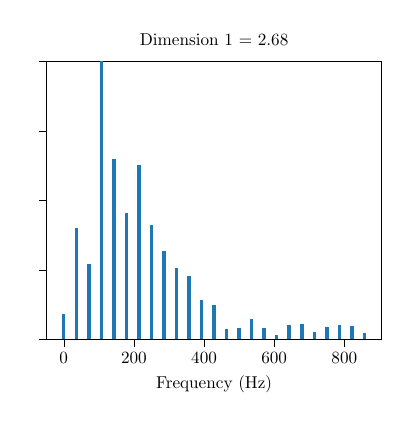
\begin{tikzpicture}[scale=0.62]

\definecolor{darkgray176}{RGB}{176,176,176}
\definecolor{steelblue31119180}{RGB}{31,119,180}

\begin{axis}[
yticklabel={\empty},
tick align=outside,
tick pos=left,
x grid style={darkgray176},
xlabel={Frequency (Hz)},
xmin=-48.3571428571429, xmax=905.5,
xtick style={color=black},
y grid style={darkgray176},
%ylabel={Magnitude},
ymin=0, ymax=4,
title={Dimension 1 = 2.68},
ytick style={color=black}
]
\draw[draw=none,fill=steelblue31119180] (axis cs:-5,0) rectangle (axis cs:5,0.363293109461665);
\draw[draw=none,fill=steelblue31119180] (axis cs:30.7142857142857,0) rectangle (axis cs:40.7142857142857,1.59671692845371);
\draw[draw=none,fill=steelblue31119180] (axis cs:66.4285714285714,0) rectangle (axis cs:76.4285714285714,1.08375129075336);
\draw[draw=none,fill=steelblue31119180] (axis cs:102.142857142857,0) rectangle (axis cs:112.142857142857,5.72028640718505);
\draw[draw=none,fill=steelblue31119180] (axis cs:137.857142857143,0) rectangle (axis cs:147.857142857143,2.60109171070077);
\draw[draw=none,fill=steelblue31119180] (axis cs:173.571428571429,0) rectangle (axis cs:183.571428571429,1.82230187959835);
\draw[draw=none,fill=steelblue31119180] (axis cs:209.285714285714,0) rectangle (axis cs:219.285714285714,2.50466396839656);
\draw[draw=none,fill=steelblue31119180] (axis cs:245,0) rectangle (axis cs:255,1.64154431128106);
\draw[draw=none,fill=steelblue31119180] (axis cs:280.714285714286,0) rectangle (axis cs:290.714285714286,1.2779936763853);
\draw[draw=none,fill=steelblue31119180] (axis cs:316.428571428571,0) rectangle (axis cs:326.428571428571,1.02566988726104);
\draw[draw=none,fill=steelblue31119180] (axis cs:352.142857142857,0) rectangle (axis cs:362.142857142857,0.906444113984638);
\draw[draw=none,fill=steelblue31119180] (axis cs:387.857142857143,0) rectangle (axis cs:397.857142857143,0.567573738688084);
\draw[draw=none,fill=steelblue31119180] (axis cs:423.571428571429,0) rectangle (axis cs:433.571428571429,0.497884322563813);
\draw[draw=none,fill=steelblue31119180] (axis cs:459.285714285714,0) rectangle (axis cs:469.285714285714,0.143370970638671);
\draw[draw=none,fill=steelblue31119180] (axis cs:495,0) rectangle (axis cs:505,0.158030205491621);
\draw[draw=none,fill=steelblue31119180] (axis cs:530.714285714286,0) rectangle (axis cs:540.714285714286,0.287791882784369);
\draw[draw=none,fill=steelblue31119180] (axis cs:566.428571428571,0) rectangle (axis cs:576.428571428571,0.164560600100172);
\draw[draw=none,fill=steelblue31119180] (axis cs:602.142857142857,0) rectangle (axis cs:612.142857142857,0.0653538748355305);
\draw[draw=none,fill=steelblue31119180] (axis cs:637.857142857143,0) rectangle (axis cs:647.857142857143,0.209706204538538);
\draw[draw=none,fill=steelblue31119180] (axis cs:673.571428571429,0) rectangle (axis cs:683.571428571429,0.216581742305538);
\draw[draw=none,fill=steelblue31119180] (axis cs:709.285714285714,0) rectangle (axis cs:719.285714285714,0.104565114650486);
\draw[draw=none,fill=steelblue31119180] (axis cs:745,0) rectangle (axis cs:755,0.18370350932939);
\draw[draw=none,fill=steelblue31119180] (axis cs:780.714285714286,0) rectangle (axis cs:790.714285714286,0.206670350113575);
\draw[draw=none,fill=steelblue31119180] (axis cs:816.428571428571,0) rectangle (axis cs:826.428571428571,0.196489132073225);
\draw[draw=none,fill=steelblue31119180] (axis cs:852.142857142857,0) rectangle (axis cs:862.142857142857,0.0885177801919891);
\end{axis}

\end{tikzpicture}

	\end{subfigure}
	
	\vspace{0.5cm} % Adjust vertical spacing between rows
	
	\begin{subfigure}{0.36\textwidth}
		\centering
		% This file was created with tikzplotlib v0.10.1.
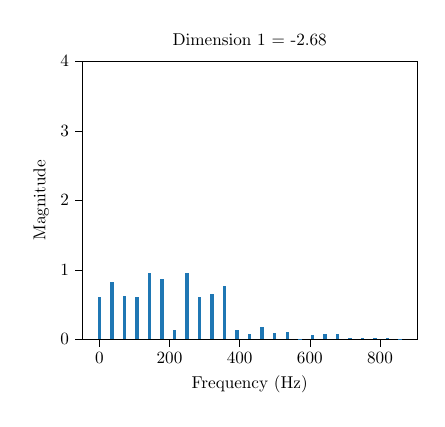
\begin{tikzpicture}[scale=0.62]

\definecolor{darkgray176}{RGB}{176,176,176}
\definecolor{steelblue31119180}{RGB}{31,119,180}

\begin{axis}[
tick align=outside,
tick pos=left,
x grid style={darkgray176},
xlabel={Frequency (Hz)},
xmin=-48.3571428571429, xmax=905.5,
xtick style={color=black},
y grid style={darkgray176},
ylabel={Magnitude},
ymin=0, ymax=4,
title={Dimension 1 = -2.68},
ytick style={color=black}
]
\draw[draw=none,fill=steelblue31119180] (axis cs:-5,0) rectangle (axis cs:5,0.605088098905981);
\draw[draw=none,fill=steelblue31119180] (axis cs:30.7142857142857,0) rectangle (axis cs:40.7142857142857,0.824946037495217);
\draw[draw=none,fill=steelblue31119180] (axis cs:66.4285714285714,0) rectangle (axis cs:76.4285714285714,0.618337924452538);
\draw[draw=none,fill=steelblue31119180] (axis cs:102.142857142857,0) rectangle (axis cs:112.142857142857,0.606547406467815);
\draw[draw=none,fill=steelblue31119180] (axis cs:137.857142857143,0) rectangle (axis cs:147.857142857143,0.952736687378679);
\draw[draw=none,fill=steelblue31119180] (axis cs:173.571428571429,0) rectangle (axis cs:183.571428571429,0.867459344161617);
\draw[draw=none,fill=steelblue31119180] (axis cs:209.285714285714,0) rectangle (axis cs:219.285714285714,0.142171590262196);
\draw[draw=none,fill=steelblue31119180] (axis cs:245,0) rectangle (axis cs:255,0.959357311317153);
\draw[draw=none,fill=steelblue31119180] (axis cs:280.714285714286,0) rectangle (axis cs:290.714285714286,0.614147542320182);
\draw[draw=none,fill=steelblue31119180] (axis cs:316.428571428571,0) rectangle (axis cs:326.428571428571,0.651510920840633);
\draw[draw=none,fill=steelblue31119180] (axis cs:352.142857142857,0) rectangle (axis cs:362.142857142857,0.767848611698322);
\draw[draw=none,fill=steelblue31119180] (axis cs:387.857142857143,0) rectangle (axis cs:397.857142857143,0.130737421425031);
\draw[draw=none,fill=steelblue31119180] (axis cs:423.571428571429,0) rectangle (axis cs:433.571428571429,0.0781024768115382);
\draw[draw=none,fill=steelblue31119180] (axis cs:459.285714285714,0) rectangle (axis cs:469.285714285714,0.174989028847861);
\draw[draw=none,fill=steelblue31119180] (axis cs:495,0) rectangle (axis cs:505,0.0957224281064073);
\draw[draw=none,fill=steelblue31119180] (axis cs:530.714285714286,0) rectangle (axis cs:540.714285714286,0.105812453640171);
\draw[draw=none,fill=steelblue31119180] (axis cs:566.428571428571,0) rectangle (axis cs:576.428571428571,0.00668246230492007);
\draw[draw=none,fill=steelblue31119180] (axis cs:602.142857142857,0) rectangle (axis cs:612.142857142857,0.0584750394429784);
\draw[draw=none,fill=steelblue31119180] (axis cs:637.857142857143,0) rectangle (axis cs:647.857142857143,0.0829703251371982);
\draw[draw=none,fill=steelblue31119180] (axis cs:673.571428571429,0) rectangle (axis cs:683.571428571429,0.0786316144734407);
\draw[draw=none,fill=steelblue31119180] (axis cs:709.285714285714,0) rectangle (axis cs:719.285714285714,0.0183265263662661);
\draw[draw=none,fill=steelblue31119180] (axis cs:745,0) rectangle (axis cs:755,0.0136594016374186);
\draw[draw=none,fill=steelblue31119180] (axis cs:780.714285714286,0) rectangle (axis cs:790.714285714286,0.0150421133154433);
\draw[draw=none,fill=steelblue31119180] (axis cs:816.428571428571,0) rectangle (axis cs:826.428571428571,0.0199113615327003);
\draw[draw=none,fill=steelblue31119180] (axis cs:852.142857142857,0) rectangle (axis cs:862.142857142857,0.00824199961136327);
\end{axis}

\end{tikzpicture}

	\end{subfigure}\hfill
	\begin{subfigure}{0.3\textwidth}
		\centering
		% This file was created with tikzplotlib v0.10.1.
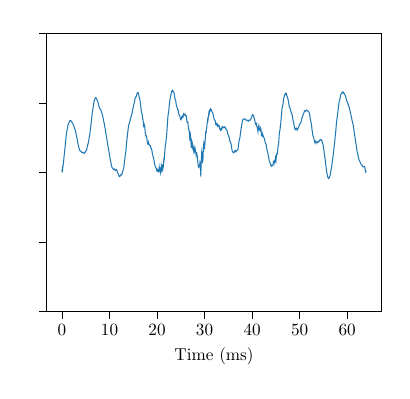
\begin{tikzpicture}[scale=0.62]

\definecolor{darkgray176}{RGB}{176,176,176}
\definecolor{steelblue31119180}{RGB}{31,119,180}

\begin{axis}[
yticklabel={\empty},
tick align=outside,
tick pos=left,
x grid style={darkgray176},
xlabel={Time (ms)},
xmin=-3.2, xmax=67.2,
xtick style={color=black},
y grid style={darkgray176},
% ylabel={Amplitude},
% ymin=-0.15, ymax=0.15,
ymin=-0.1, ymax=0.1,
ytick style={color=black}
]
\addplot [semithick, steelblue31119180]
table {%
0 0
0.0625610948191593 0.00267421979664707
0.125122189638319 0.00195263445792485
0.187683284457478 0.00448575329658223
0.250244379276637 0.00506307051416017
0.312805474095797 0.00741872769886972
0.375366568914956 0.00896099196129705
0.437927663734115 0.0115803680341702
0.500488758553275 0.0133900876509304
0.563049853372434 0.0151754755341063
0.625610948191593 0.0175304286389494
0.688172043010753 0.0195827149455586
0.750733137829912 0.0220035516719752
0.813294232649071 0.0241572310672827
0.875855327468231 0.0260075675241671
0.93841642228739 0.0276190532682753
1.00097751710655 0.029011056083869
1.06353861192571 0.0303319803605681
1.12609970674487 0.0314772311226626
1.18866080156403 0.0323503866813574
1.25122189638319 0.0340090383259345
1.31378299120235 0.0342868589673224
1.37634408602151 0.034962264941104
1.43890518084066 0.0355454103753539
1.50146627565982 0.0360117456070052
1.56402737047898 0.0365307936963797
1.62658846529814 0.0370469956639663
1.6891495601173 0.0372855405697375
1.75171065493646 0.0373638160362883
1.81427174975562 0.0371841114243804
1.87683284457478 0.0371509336557818
1.93939393939394 0.0367688526484099
2.0019550342131 0.0364753106155616
2.06451612903226 0.0361838696464416
2.12707722385142 0.0359691435804378
2.18963831867058 0.0355138606187011
2.25219941348974 0.0352915312351981
2.3147605083089 0.0347998261102134
2.37732160312805 0.0344101194336005
2.43988269794721 0.0336631536920749
2.50244379276637 0.0331262272681571
2.56500488758553 0.0324098647864333
2.62756598240469 0.0318902237095004
2.69012707722385 0.0313611501975318
2.75268817204301 0.030779401080743
2.81524926686217 0.0301372612829257
2.87781036168133 0.0291732079745475
2.94037145650049 0.0278471793837386
3.00293255131965 0.026998937900159
3.06549364613881 0.0261555616457092
3.12805474095797 0.0251639858926059
3.19061583577713 0.0240808387786762
3.25317693059629 0.0226956488526374
3.31573802541544 0.0215881998074457
3.3782991202346 0.0205637725818454
3.44086021505376 0.0194245896512462
3.50342130987292 0.0185915641158907
3.56598240469208 0.0176511272853595
3.62854349951124 0.016837186412203
3.6911045943304 0.0160462343054783
3.75366568914956 0.0156823699676658
3.81622678396872 0.0154439510553638
3.87878787878788 0.0154666042124683
3.94134897360704 0.0152564826052734
4.0039100684262 0.0150434925245487
4.06647116324536 0.01496300729445
4.12903225806452 0.0145273268102638
4.19159335288368 0.0143023412947781
4.25415444770283 0.0141885221670887
4.31671554252199 0.0143579145090496
4.37927663734115 0.0143627272509148
4.44183773216031 0.0143107777445023
4.50439882697947 0.0143003093455631
4.56695992179863 0.0140994674365017
4.62952101661779 0.0139923333422529
4.69208211143695 0.0136977836183788
4.75464320625611 0.013858715826072
4.81720430107527 0.0140708540115626
4.87976539589443 0.0146523808071778
4.94232649071359 0.0149836221114456
5.00488758553275 0.0151687482169821
5.06744868035191 0.0155991362598984
5.13000977517107 0.0159412591371281
5.19257086999022 0.0162529259035227
5.25513196480938 0.017360441337539
5.31769305962854 0.0182014699926999
5.3802541544477 0.0193291187581341
5.44281524926686 0.0200854901912625
5.50537634408602 0.0208316617795537
5.56793743890518 0.0217071624084914
5.63049853372434 0.0229126865049698
5.6930596285435 0.0242266035106175
5.75562072336266 0.0256323526474126
5.81818181818182 0.0267178274013779
5.88074291300098 0.0283921178146279
5.94330400782014 0.0298888944198659
6.0058651026393 0.0314556878562634
6.06842619745846 0.0335125506820042
6.13098729227761 0.0353603800185178
6.19354838709677 0.0371862264169801
6.25610948191593 0.0392754322130921
6.31867057673509 0.0411166230822938
6.38123167155425 0.0428521498174699
6.44379276637341 0.0441375720776246
6.50635386119257 0.0457053787929834
6.56891495601173 0.0472871441710904
6.63147605083089 0.048761960190019
6.69403714565005 0.0498478819788201
6.75659824046921 0.050987220705211
6.81915933528837 0.0516526354504121
6.88172043010753 0.052490993072429
6.94428152492669 0.0530063456738275
7.00684261974585 0.0534649434775289
7.069403714565 0.0537074036634038
7.13196480938416 0.0537072170656885
7.19452590420332 0.0535349667596677
7.25708699902248 0.0530148078673833
7.31964809384164 0.0528068320274003
7.3822091886608 0.0521574912434362
7.44477028347996 0.0515556330096162
7.50733137829912 0.0511457352595857
7.56989247311828 0.0503554332160181
7.63245356793744 0.0496244228928407
7.6950146627566 0.0487227421199297
7.75757575757576 0.0479266882281412
7.82013685239492 0.0471831423031095
7.88269794721408 0.046654381715526
7.94525904203324 0.0460351152001413
8.00782013685239 0.0457550140146898
8.07038123167155 0.0454348212550462
8.13294232649071 0.0452133226112798
8.19550342130987 0.0445972337685198
8.25806451612903 0.0439055550603136
8.32062561094819 0.0433501996252893
8.38318670576735 0.0427576806942476
8.44574780058651 0.0420135908768324
8.50830889540567 0.0413939108542246
8.57086999022483 0.040383708649629
8.63343108504399 0.0394220507029127
8.69599217986315 0.0382373149225439
8.75855327468231 0.0370243414417128
8.82111436950147 0.0361064742824549
8.88367546432062 0.0353182733026156
8.94623655913978 0.034049863776853
9.00879765395894 0.0328304045656122
9.0713587487781 0.0317752120300822
9.13391984359726 0.0303793267955965
9.19648093841642 0.0287503501471361
9.25904203323558 0.0277123870792364
9.32160312805474 0.0264058492072691
9.3841642228739 0.0252075347437624
9.44672531769306 0.0238300412674803
9.50928641251222 0.0225178186025176
9.57184750733138 0.0210519984932589
9.63440860215054 0.0198594470538439
9.6969696969697 0.0187120908363299
9.75953079178886 0.0173988586176962
9.82209188660802 0.0162397695983872
9.88465298142718 0.0150185930283188
9.94721407624633 0.0135728019423499
10.0097751710655 0.0123385272515921
10.0723362658847 0.0110240861762566
10.1348973607038 0.00961095098504398
10.197458455523 0.00825266510554073
10.2600195503421 0.0075971999443259
10.3225806451613 0.00651535481935547
10.3851417399804 0.00549221840684365
10.4477028347996 0.00441473745945787
10.5102639296188 0.00380801213386297
10.5728250244379 0.00333096788884782
10.6353861192571 0.0030224520516448
10.6979472140762 0.00274330640315485
10.7605083088954 0.00251342399357176
10.8230694037146 0.00208306508657695
10.8856304985337 0.00217947526630069
10.9481915933529 0.00227255503649761
11.010752688172 0.00244182444387867
11.0733137829912 0.00224105331533291
11.1358748778104 0.00175680994681599
11.1984359726295 0.00137892175367501
11.2609970674487 0.0013601645838218
11.3235581622678 0.001649708713779
11.386119257087 0.00193779625522951
11.4486803519062 0.00198972274349931
11.5112414467253 0.00166785174057631
11.5738025415445 0.00142994691833548
11.6363636363636 0.00061140903695063
11.6989247311828 -0.000307942650491191
11.761485826002 -0.000503915605132532
11.8240469208211 -0.00113124737401337
11.8866080156403 -0.00155196709236092
11.9491691104594 -0.00214502619049591
12.0117302052786 -0.00279614021264213
12.0742913000978 -0.00304161296212429
12.1368523949169 -0.00297893156076282
12.1994134897361 -0.00285662688817447
12.2619745845552 -0.00236801814582865
12.3245356793744 -0.0021942504504122
12.3870967741935 -0.00160614665477507
12.4496578690127 -0.00156108215123502
12.5122189638319 -0.0018311939707512
12.574780058651 -0.00173706366869012
12.6373411534702 -0.000912511972519309
12.6999022482893 -0.000196902665836721
12.7624633431085 0.000736978850013351
12.8250244379277 0.00106108622335968
12.8875855327468 0.00214182240806542
12.950146627566 0.00270913908383713
13.0127077223851 0.00340024156829129
13.0752688172043 0.00556807706673299
13.1378299120235 0.00725564627725183
13.2003910068426 0.00904701511400187
13.2629521016618 0.0112418273021399
13.3255131964809 0.0124709883655621
13.3880742913001 0.0139866596431938
13.4506353861193 0.0154722398884398
13.5131964809384 0.0179199806613919
13.5757575757576 0.0204215760935437
13.6383186705767 0.0226809065843607
13.7008797653959 0.0248251628578583
13.7634408602151 0.0266148869789416
13.8260019550342 0.0284216282261082
13.8885630498534 0.0303372205931508
13.9511241446725 0.0320307074273087
14.0136852394917 0.0336226689249627
14.0762463343109 0.0342720239436871
14.13880742913 0.0349491323751351
14.2013685239492 0.0356921560931241
14.2639296187683 0.0364141654485394
14.3264907135875 0.0373742953598325
14.3890518084066 0.0380467732554394
14.4516129032258 0.0389382684182736
14.514173998045 0.039927060713123
14.5767350928641 0.0404909389459493
14.6392961876833 0.0411950073032872
14.7018572825024 0.0419001485442311
14.7644183773216 0.0429625525753781
14.8269794721408 0.0438603695558488
14.8895405669599 0.0452642597727849
14.9521016617791 0.0463684541105001
15.0146627565982 0.0474161693220002
15.0772238514174 0.0484258940230367
15.1397849462366 0.048982958699907
15.2023460410557 0.0497803344033506
15.2649071358749 0.051131768807594
15.327468230694 0.0521033428106839
15.3900293255132 0.0531876813511083
15.4525904203324 0.0538189128325307
15.5151515151515 0.0541310210458257
15.5777126099707 0.0543522023735158
15.6402737047898 0.0549303894463785
15.702834799609 0.0555825384328267
15.7653958944282 0.0564133933201826
15.8279569892473 0.056831538196533
15.8905180840665 0.0572587951329534
15.9530791788856 0.057280189141937
16.0156402737048 0.0573616571822736
16.0782013685239 0.056989228402065
16.1407624633431 0.0559466459741952
16.2033235581623 0.0549218033787267
16.2658846529814 0.0539930620970876
16.3284457478006 0.0531750289925382
16.3910068426197 0.0521099569871366
16.4535679374389 0.0510703175386026
16.5161290322581 0.0493302415575712
16.5786901270772 0.0474945895286424
16.6412512218964 0.0456468005039213
16.7038123167155 0.0437111058040274
16.7663734115347 0.0426618811835554
16.8289345063539 0.0419866980607908
16.891495601173 0.0413465699197348
16.9540566959922 0.0398208843953798
17.0166177908113 0.0385363369120443
17.0791788856305 0.0372270050723532
17.1417399804497 0.0345423184062117
17.2043010752688 0.032461166021324
17.266862170088 0.0347551361239813
17.3294232649071 0.0341661413175619
17.3919843597263 0.0338865765739134
17.4545454545455 0.0314861332828348
17.5171065493646 0.0286533663273295
17.5796676441838 0.0271085365361307
17.6422287390029 0.0262852582228411
17.7047898338221 0.0263691197621945
17.7673509286412 0.0262591917002219
17.8299120234604 0.0251460206091317
17.8924731182796 0.023419109804015
17.9550342130987 0.0213664465766848
18.0175953079179 0.0208063320833043
18.080156402737 0.0203971048855275
18.1427174975562 0.0208537711262091
18.2052785923754 0.0216071604644536
18.2678396871945 0.020109887729205
18.3304007820137 0.0199684586124686
18.3929618768328 0.0197349161051673
18.455522971652 0.0194785226671752
18.5180840664712 0.0194128193889807
18.5806451612903 0.0193844509701575
18.6432062561095 0.0188214922176341
18.7057673509286 0.0173547650001878
18.7683284457478 0.0172885383187064
18.830889540567 0.0166502374325417
18.8934506353861 0.0162434242228783
18.9560117302053 0.0150629650757722
19.0185728250244 0.013391328265459
19.0811339198436 0.0127082065490683
19.1436950146628 0.0115744774434661
19.2062561094819 0.0109363535085906
19.2688172043011 0.0104743799254779
19.3313782991202 0.00898958691272917
19.3939393939394 0.00790707682344046
19.4565004887586 0.0066469337168502
19.5190615835777 0.00564898771733657
19.5816226783969 0.0047800187185363
19.644183773216 0.00409872611968224
19.7067448680352 0.00366864474681465
19.7693059628544 0.00332232838895314
19.8318670576735 0.00288059430803197
19.8944281524927 0.00273982084238809
19.9569892473118 0.000845879196159301
20.019550342131 0.000760033273321092
20.0821114369501 0.00095205489120001
20.1446725317693 0.0019063416846599
20.2072336265885 0.00162790942926211
20.2697947214076 0.000875847490608168
20.3323558162268 0.000575767573286014
20.3949169110459 0.00160671152786251
20.4574780058651 0.00388647337332149
20.5200391006843 0.00233205468489453
20.5826001955034 0.00152916488540837
20.6451612903226 0.00328123563479993
20.7077223851417 0.00326864568303582
20.7702834799609 -0.00020999720325568
20.8328445747801 0.000763068778598764
20.8954056695992 0.00438050786442945
20.9579667644184 0.0029384327555332
21.0205278592375 0.000206796255760179
21.0830889540567 0.00278985447351359
21.1456500488759 0.00508365880075263
21.208211143695 0.00488976083280753
21.2707722385142 0.00338998097718811
21.3333333333333 0.00464094616472721
21.3958944281525 0.00786668587683582
21.4584555229717 0.0097706981789856
21.5210166177908 0.00937353533384038
21.58357771261 0.0119085969113884
21.6461388074291 0.0154543465107155
21.7086999022483 0.0183054468160238
21.7712609970674 0.0201115640770655
21.8338220918866 0.0206162288205977
21.8963831867058 0.0229037094675551
21.9589442815249 0.0247902948616886
22.0215053763441 0.0266693644826451
22.0840664711632 0.030081022257679
22.1466275659824 0.0328973525659867
22.2091886608016 0.0361175192438088
22.2717497556207 0.0395221697477913
22.3343108504399 0.041304173204731
22.396871945259 0.0427716355006104
22.4594330400782 0.0439727842436333
22.5219941348974 0.04629844911615
22.5845552297165 0.0490542658088494
22.6471163245357 0.0508796651724759
22.7096774193548 0.0520982259223538
22.772238514174 0.0532420461729737
22.8347996089932 0.0545685695609914
22.8973607038123 0.0551733477560044
22.9599217986315 0.0559879976305619
23.0224828934506 0.0578949249723702
23.0850439882698 0.0583804640755101
23.147605083089 0.0584930904439031
23.2101661779081 0.0588970233377648
23.2727272727273 0.0583844416859475
23.3352883675464 0.0586766382225972
23.3978494623656 0.0583387540593263
23.4604105571848 0.0581928974350701
23.5229716520039 0.0575271020438577
23.5855327468231 0.0569285704942742
23.6480938416422 0.0559307399787599
23.7106549364614 0.0543003477199861
23.7732160312805 0.0534002241184198
23.8357771260997 0.0520780251260377
23.8983382209189 0.0516900767864457
23.960899315738 0.0508313895888692
24.0234604105572 0.049175866521742
24.0860215053763 0.0479400197584783
24.1485826001955 0.0473373903895665
24.2111436950147 0.046511578878874
24.2737047898338 0.0462514713264543
24.336265884653 0.0451448697848054
24.3988269794721 0.0451817311991083
24.4613880742913 0.0443530065114023
24.5239491691105 0.0426578202784673
24.5865102639296 0.0416546216196329
24.6490713587488 0.0413088361156389
24.7116324535679 0.041108225174576
24.7741935483871 0.0408650341654016
24.8367546432063 0.0398515648812143
24.8993157380254 0.038847956440447
24.9618768328446 0.0380346358281252
25.0244379276637 0.0378304746854078
25.0869990224829 0.0382387661689188
25.1495601173021 0.0390100164114992
25.2121212121212 0.0399538556283171
25.2746823069404 0.040413034577305
25.3372434017595 0.0400065938966715
25.3998044965787 0.0394734188400843
25.4623655913978 0.0394740778832666
25.524926686217 0.0411028750513918
25.5874877810362 0.0420756560485384
25.6500488758553 0.0417780720757162
25.7126099706745 0.0412677814774324
25.7751710654936 0.041175230032057
25.8377321603128 0.0413646532599527
25.900293255132 0.0417800190697405
25.9628543499511 0.0412614583269941
26.0254154447703 0.0406542915544989
26.0879765395894 0.0408050164667742
26.1505376344086 0.0405792076621325
26.2130987292278 0.0390043036023543
26.2756598240469 0.0368666124866068
26.3382209188661 0.0360929401389315
26.4007820136852 0.0362097313818781
26.4633431085044 0.036331480986212
26.5259042033236 0.0345905183860896
26.5884652981427 0.031986461903168
26.6510263929619 0.031094742556515
26.713587487781 0.0309626471546214
26.7761485826002 0.0293936625811274
26.8387096774194 0.0263035376706431
26.9012707722385 0.0239715223744118
26.9638318670577 0.0245473122229674
27.0263929618768 0.026747274624943
27.088954056696 0.0248879576893933
27.1515151515152 0.0209304007955573
27.2140762463343 0.0176937769814408
27.2766373411535 0.0196157470454743
27.3391984359726 0.0221516430880492
27.4017595307918 0.0213706412317117
27.4643206256109 0.0188635372914527
27.5268817204301 0.0167689943505872
27.5894428152493 0.0163053760518077
27.6520039100684 0.0177176835621732
27.7145650048876 0.0165713070960076
27.7771260997067 0.0141103166617082
27.8396871945259 0.0146560471428454
27.9022482893451 0.0159809314031318
27.9648093841642 0.0179326702619403
28.0273704789834 0.0170464531690581
28.0899315738025 0.0151981798565982
28.1524926686217 0.0144559601349128
28.2150537634409 0.0127864169377473
28.27761485826 0.0140569939160627
28.3401759530792 0.0141271333486017
28.4027370478983 0.0123410444444488
28.4652981427175 0.0116867676508392
28.5278592375367 0.00907893372355493
28.5904203323558 0.00709933834013876
28.652981427175 0.00512608153816542
28.7155425219941 0.00378594341035113
28.7781036168133 0.00356751068050036
28.8406647116325 0.00437589089148555
28.9032258064516 0.00465376368693767
28.9657869012708 0.00537902522078357
29.0283479960899 0.00695361941506611
29.0909090909091 0.00594923797656189
29.1534701857282 0.0013902217881683
29.2160312805474 -0.00304396178496898
29.2785923753666 0.00566547975228154
29.3411534701857 0.0108653606896089
29.4037145650049 0.014694018147427
29.466275659824 0.0133876833037809
29.5288367546432 0.0101675867400736
29.5913978494624 0.00803752129356707
29.6539589442815 0.00901241266766776
29.7165200391007 0.0144135524133696
29.7790811339198 0.0189351138667015
29.841642228739 0.0207817511103195
29.9042033235582 0.0193139174816545
29.9667644183773 0.0165541066113543
30.0293255131965 0.0189539923051323
30.0918866080156 0.0218169781491379
30.1544477028348 0.0246398184022421
30.217008797654 0.0282433863696465
30.2795698924731 0.0278777189913296
30.3421309872923 0.0289339464911617
30.4046920821114 0.0309737586632065
30.4672531769306 0.0327821483513302
30.5298142717498 0.0346808726039013
30.5923753665689 0.0366036100777363
30.6549364613881 0.0380971568562855
30.7174975562072 0.0375351592286591
30.7800586510264 0.0395417567124028
30.8426197458456 0.0406106800015721
30.9051808406647 0.0431468461276936
30.9677419354839 0.0440592289932313
31.030303030303 0.0431223926557736
31.0928641251222 0.044251091953072
31.1554252199413 0.044091906240128
31.2179863147605 0.0447321454734921
31.2805474095797 0.0457030936278119
31.3431085043988 0.0453781697494893
31.405669599218 0.0451644942153496
31.4682306940371 0.0443997886414227
31.5307917888563 0.0437652633369756
31.5933528836755 0.0434029524452176
31.6559139784946 0.043035791225491
31.7184750733138 0.0426897188741441
31.7810361681329 0.0420002157354722
31.8435972629521 0.0409411973268056
31.9061583577713 0.039571873412148
31.9687194525904 0.0386384047371202
32.0312805474096 0.0383785877573438
32.0938416422287 0.0375490882092557
32.1564027370479 0.0375753101944661
32.2189638318671 0.0374420748537412
32.2815249266862 0.0360706945788388
32.3440860215054 0.0350615131037851
32.4066471163245 0.0339929430507932
32.4692082111437 0.0340246002345491
32.5317693059629 0.0349592938636842
32.594330400782 0.0352224107842641
32.6568914956012 0.034789714257607
32.7194525904203 0.0336865213565812
32.7820136852395 0.0331596681176305
32.8445747800587 0.0334299338702932
32.9071358748778 0.0338081808875471
32.969696969697 0.033365224911408
33.0322580645161 0.0329333330474554
33.0948191593353 0.0332109972266508
33.1573802541544 0.0320883396838155
33.2199413489736 0.0309007317046266
33.2825024437928 0.0308718603716131
33.3450635386119 0.030459921162499
33.4076246334311 0.0313069512603307
33.4701857282502 0.0315470496121565
33.5327468230694 0.0310009366223627
33.5953079178886 0.0306450518563696
33.6578690127077 0.0318058445295892
33.7204301075269 0.0329603675392366
33.782991202346 0.0327633887562147
33.8455522971652 0.032416258422423
33.9081133919844 0.0322558210119387
33.9706744868035 0.0320788991918837
34.0332355816227 0.0323125378903318
34.0957966764418 0.0326428515973154
34.158357771261 0.0326298984297472
34.2209188660802 0.032318359519467
34.2834799608993 0.0326219256421076
34.3460410557185 0.0323100589062811
34.4086021505376 0.0318218369277254
34.4711632453568 0.0310809285082251
34.533724340176 0.0310058263226076
34.5962854349951 0.0309875087370096
34.6588465298143 0.0306313110466315
34.7214076246334 0.0300611066044775
34.7839687194526 0.0293552047379118
34.8465298142717 0.0284407946480509
34.9090909090909 0.0275458454747092
34.9716520039101 0.0268777255023505
35.0342130987292 0.0267992109508196
35.0967741935484 0.0259139400816733
35.1593352883675 0.0252057173592516
35.2218963831867 0.0244404716182314
35.2844574780059 0.0227533189738251
35.347018572825 0.0225678494751803
35.4095796676442 0.0221244483268506
35.4721407624633 0.0217717170190951
35.5347018572825 0.0210364933925902
35.5972629521017 0.0201191887521674
35.6598240469208 0.0188929513752286
35.72238514174 0.0170571037685591
35.7849462365591 0.0159716786396119
35.8475073313783 0.0150278387563931
35.9100684261975 0.01489631146127
35.9726295210166 0.0146592597305076
36.0351906158358 0.0141087751125485
36.0977517106549 0.014124936951308
36.1603128054741 0.014254863567847
36.2228739002933 0.0143559359483792
36.2854349951124 0.0151110854862897
36.3479960899316 0.0150740762566192
36.4105571847507 0.0157257782082316
36.4731182795699 0.0156458070681941
36.5356793743891 0.0150090577654388
36.5982404692082 0.0147384244052808
36.6608015640274 0.015120394850188
36.7233626588465 0.0154524166027734
36.7859237536657 0.0158782299892032
36.8484848484849 0.0158998847685077
36.911045943304 0.0161424008337371
36.9736070381232 0.0162015636984117
37.0361681329423 0.0167102424422405
37.0987292277615 0.0182204747960365
37.1612903225806 0.0200580241939714
37.2238514173998 0.0217561341133897
37.286412512219 0.0231641612652023
37.3489736070381 0.0238318093219373
37.4115347018573 0.0247525442883241
37.4740957966764 0.025644510700381
37.5366568914956 0.0275202778514879
37.5992179863148 0.0292770331534298
37.6617790811339 0.0308391401746318
37.7243401759531 0.0322980790063083
37.7869012707722 0.0334602463116482
37.8494623655914 0.0347619480904072
37.9120234604106 0.0359631676139457
37.9745845552297 0.0368996791847465
38.0371456500489 0.0378674757434738
38.099706744868 0.0381146148939636
38.1622678396872 0.0383059976245563
38.2248289345064 0.0384774612279232
38.2873900293255 0.0383171840049217
38.3499511241447 0.0384484256489361
38.4125122189638 0.0384597241212109
38.475073313783 0.0384790841216915
38.5376344086022 0.0383175552011498
38.6001955034213 0.0377998699016235
38.6627565982405 0.0377321959448612
38.7253176930596 0.0376487938124588
38.7878787878788 0.0376734474504536
38.8504398826979 0.0375150216967304
38.9130009775171 0.0375846544897888
38.9755620723363 0.0374904452902306
39.0381231671554 0.0374442960608128
39.1006842619746 0.0372936971420067
39.1632453567937 0.0369457174420269
39.2258064516129 0.0368236430710362
39.2883675464321 0.0373380606245697
39.3509286412512 0.0374558800476387
39.4134897360704 0.0376636466049641
39.4760508308895 0.0376178475528344
39.5386119257087 0.0375941767250775
39.6011730205279 0.0375067810814751
39.663734115347 0.0377316429959801
39.7262952101662 0.0381126951568287
39.7888563049853 0.0388838746188935
39.8514173998045 0.0394202564840268
39.9139784946237 0.0397456081043328
39.9765395894428 0.040315290339444
40.039100684262 0.0412298003457421
40.1016617790811 0.0414068146316537
40.1642228739003 0.0410492199574136
40.2267839687195 0.0411880649189271
40.2893450635386 0.0409462820694856
40.3519061583578 0.0401449904195374
40.4144672531769 0.0390465733406743
40.4770283479961 0.0386799932662343
40.5395894428152 0.0376865399668206
40.6021505376344 0.0366314517394189
40.6647116324536 0.0358175872347135
40.7272727272727 0.0348084318366918
40.7898338220919 0.0344157486531304
40.852394916911 0.0347675312081041
40.9149560117302 0.0350688882335977
40.9775171065494 0.0333061736634225
41.0400782013685 0.032600074356471
41.1026392961877 0.0321379145088434
41.1652003910068 0.0307046050080194
41.227761485826 0.0294969624176053
41.2903225806452 0.0325823667188806
41.3528836754643 0.0329074016895112
41.4154447702835 0.0337845209570836
41.4780058651026 0.0325840122975912
41.5405669599218 0.0306703675909738
41.603128054741 0.0305694714953298
41.6656891495601 0.030171353113223
41.7282502443793 0.031143564140954
41.7908113391984 0.0318894302554407
41.8533724340176 0.0306748176468782
41.9159335288368 0.0292985609669752
41.9784946236559 0.0267994198347292
42.0410557184751 0.0260753441394424
42.1036168132942 0.026039359364604
42.1661779081134 0.0267842792553549
42.2287390029325 0.0277295210439701
42.2913000977517 0.0265493077660236
42.3538611925709 0.0261299217016029
42.41642228739 0.0255084721661034
42.4789833822092 0.0248335181486921
42.5415444770283 0.0245418480742187
42.6041055718475 0.0241732470297918
42.6666666666667 0.0232807192951441
42.7292277614858 0.0216111164933338
42.791788856305 0.0214149535488873
42.8543499511241 0.0207516336130781
42.9169110459433 0.0204178342306194
42.9794721407625 0.0192357806592655
43.0420332355816 0.0175879018878307
43.1045943304008 0.0168795692693453
43.1671554252199 0.0155753857808466
43.2297165200391 0.0148914705776224
43.2922776148583 0.0144289083986426
43.3548387096774 0.0130980704580584
43.4173998044966 0.0120939013611012
43.4799608993157 0.0108472363548108
43.5425219941349 0.00960976536497692
43.6050830889541 0.00849363266809944
43.6676441837732 0.00765429090304284
43.7302052785924 0.00705099843245797
43.7927663734115 0.00663502100866037
43.8553274682307 0.00606322959283929
43.9178885630498 0.00568777587690836
43.980449657869 0.00445893265940576
44.0430107526882 0.00439443637526804
44.1055718475073 0.00446561516380031
44.1681329423265 0.00513564554368121
44.2306940371457 0.00521406070861823
44.2932551319648 0.00499794883462341
44.355816226784 0.00488837840051945
44.4183773216031 0.00564268229753216
44.4809384164223 0.00737928005366906
44.5434995112414 0.00707713632552155
44.6060606060606 0.0070919179442254
44.6686217008798 0.00851020454551992
44.7311827956989 0.00866406987751684
44.7937438905181 0.00704828820729361
44.8563049853372 0.00816068935953627
44.9188660801564 0.0108787558229962
44.9814271749756 0.010371167922824
45.0439882697947 0.00914865583618366
45.1065493646139 0.0114646889706336
45.169110459433 0.0132357996787406
45.2316715542522 0.0134156004817954
45.2942326490714 0.0132334446288711
45.3567937438905 0.0144499974472781
45.4193548387097 0.0173056817222987
45.4819159335288 0.019130442198639
45.544477028348 0.0196244097710792
45.6070381231672 0.021854941905244
45.6695992179863 0.025132772351596
45.7321603128055 0.0278786127168762
45.7947214076246 0.0295117591614248
45.8572825024438 0.0303778906852619
45.919843597263 0.0322564648426086
45.9824046920821 0.0339553831500217
46.0449657869013 0.0358612972128688
46.1075268817204 0.0385077691847278
46.1700879765396 0.0408807266175834
46.2326490713588 0.0432648152178508
46.2952101661779 0.0456662636709091
46.3577712609971 0.046847217615224
46.4203323558162 0.0477867429458763
46.4828934506354 0.0485950412004749
46.5454545454545 0.0505165232514793
46.6080156402737 0.0525513137322018
46.6705767350929 0.0537294811593735
46.733137829912 0.0543446789913513
46.7956989247312 0.0549502618490688
46.8582600195503 0.0558704715495235
46.9208211143695 0.0559133530329487
46.9833822091887 0.0559761648194706
47.0459433040078 0.0569916450940182
47.108504398827 0.0570250419883434
47.1710654936461 0.0568927230690319
47.2336265884653 0.056640900562236
47.2961876832845 0.0551848630653011
47.3587487781036 0.0547586485437634
47.4213098729228 0.0541026841936486
47.4838709677419 0.0536307193819554
47.5464320625611 0.0527246055135891
47.6089931573803 0.0517289356664479
47.6715542521994 0.0508142424545243
47.7341153470186 0.0493116723564713
47.7966764418377 0.0481130375179989
47.8592375366569 0.0468085671821473
47.9217986314761 0.0465829856202137
47.9843597262952 0.0462157163670685
48.0469208211144 0.0452095076736729
48.1094819159335 0.0442796264532025
48.1720430107527 0.0438324161955426
48.2346041055718 0.0430557673409188
48.297165200391 0.0426278280099728
48.3597262952102 0.0418391911711686
48.4222873900293 0.041594998058904
48.4848484848485 0.0406052067198537
48.5474095796676 0.0389845076664365
48.6099706744868 0.0375579707433751
48.672531769306 0.0365544479842847
48.7350928641251 0.0357116901280244
48.7976539589443 0.0348651324756596
48.8602150537634 0.0336367660953153
48.9227761485826 0.0324083252091649
48.9853372434018 0.0313928293670552
49.0478983382209 0.0309147811563046
49.1104594330401 0.030692954686992
49.1730205278592 0.0309709876699269
49.2355816226784 0.031597696648927
49.2981427174976 0.0318774469906896
49.3607038123167 0.0314093900085195
49.4232649071359 0.0308339031047223
49.485826001955 0.0304353637648118
49.5483870967742 0.031060064812341
49.6109481915934 0.0315283893490117
49.6735092864125 0.031664160946029
49.7360703812317 0.0318912170565198
49.7986314760508 0.0325307298582757
49.86119257087 0.0333566375601152
49.9237536656891 0.0340274055474752
49.9863147605083 0.0343475082337507
50.0488758553275 0.0348904801374219
50.1114369501466 0.0352367120098508
50.1739980449658 0.0354705928521684
50.2365591397849 0.0357889670037454
50.2991202346041 0.0362658038287481
50.3616813294233 0.0370228979681944
50.4242424242424 0.0380117535929788
50.4868035190616 0.0389377374933962
50.5493646138807 0.0395894841484922
50.6119257086999 0.0399620687244924
50.6744868035191 0.0408489817802595
50.7370478983382 0.0415870843897642
50.7996089931574 0.0421664896325544
50.8621700879765 0.0424486465118498
50.9247311827957 0.04317258929293
50.9872922776149 0.0436714500341772
51.049853372434 0.0439890157977594
51.1124144672532 0.044358433877006
51.1749755620723 0.0441271898738188
51.2375366568915 0.0438700103995737
51.3000977517107 0.0442643841985296
51.3626588465298 0.0446783232221331
51.425219941349 0.0449076517597059
51.4877810361681 0.0448242272755617
51.5503421309873 0.0448317967322477
51.6129032258064 0.0444544803711676
51.6754643206256 0.0442608096459307
51.7380254154448 0.0440060031816057
51.8005865102639 0.0440069565227217
51.8631476050831 0.0439781410690626
51.9257086999022 0.0437708097043013
51.9882697947214 0.0431585281082262
52.0508308895406 0.0425149987771277
52.1133919843597 0.0415439978023428
52.1759530791789 0.0401725728239569
52.238514173998 0.0387360111447024
52.3010752688172 0.0377038967825713
52.3636363636364 0.0366723598404364
52.4261974584555 0.0354431589950652
52.4887585532747 0.0341393890137896
52.5513196480938 0.0325012071730017
52.613880742913 0.0306788693315997
52.6764418377322 0.0291148989988475
52.7390029325513 0.0275694079686208
52.8015640273705 0.0265256427610812
52.8641251221896 0.0256399043680024
52.9266862170088 0.0253011354482856
52.989247311828 0.0243811560494284
53.0518084066471 0.0233437759894605
53.1143695014663 0.0225893578046927
53.1769305962854 0.0217172744632029
53.2394916911046 0.0211648024028697
53.3020527859238 0.0224554698717647
53.3646138807429 0.0222937956649013
53.4271749755621 0.0224200454199157
53.4897360703812 0.0216772929817176
53.5522971652004 0.0212178265189757
53.6148582600196 0.0211791725736385
53.6774193548387 0.0211344315039535
53.7399804496579 0.0214040229790721
53.802541544477 0.0220809991627145
53.8651026392962 0.0223197899376455
53.9276637341153 0.0223311759542423
53.9902248289345 0.0219567615943046
54.0527859237537 0.0220094107888923
54.1153470185728 0.0223439676015258
54.177908113392 0.0227976033185497
54.2404692082111 0.0232850162427097
54.3030303030303 0.0231732385741039
54.3655913978495 0.0234766053937135
54.4281524926686 0.0236280772266937
54.4907135874878 0.0235211834136692
54.5532746823069 0.0233881529639106
54.6158357771261 0.0231276766077514
54.6783968719453 0.0227126081547867
54.7409579667644 0.0217724376825119
54.8035190615836 0.0213462827656189
54.8660801564027 0.0205169620314651
54.9286412512219 0.020012508963079
54.9912023460411 0.0188231631359659
55.0537634408602 0.0171258385863996
55.1163245356794 0.0157880976828924
55.1788856304985 0.0139106013306862
55.2414467253177 0.0122885611727615
55.3040078201369 0.0112943628152882
55.366568914956 0.0093972099688221
55.4291300097752 0.00770373364413414
55.4916911045943 0.00584246838175831
55.5542521994135 0.00412534391425572
55.6168132942326 0.00245839351913796
55.6793743890518 0.000780038147771465
55.741935483871 -0.000622202431963335
55.8044965786901 -0.00163171173256339
55.8670576735093 -0.00270341847998656
55.9296187683284 -0.00340635501547468
55.9921798631476 -0.00384208765372503
56.0547409579668 -0.00413895264551961
56.1173020527859 -0.00444098088966786
56.1798631476051 -0.00418070636558568
56.2424242424242 -0.00360199775208126
56.3049853372434 -0.00304885953118549
56.3675464320626 -0.00252012568703495
56.4301075268817 -0.0017775341027206
56.4926686217009 -0.000825290630989413
56.55522971652 0.000563787831720022
56.6177908113392 0.00183773806040063
56.6803519061584 0.00313017317954221
56.7429130009775 0.00412363140049044
56.8054740957967 0.00566291729332415
56.8680351906158 0.00711228026628844
56.930596285435 0.0089067299181153
56.9931573802542 0.0104306080102746
57.0557184750733 0.0119805407827813
57.1182795698925 0.0143055500042054
57.1808406647116 0.0158458994674193
57.2434017595308 0.0175163397931458
57.3059628543499 0.0196888505309121
57.3685239491691 0.0215753390674979
57.4310850439883 0.023990589721112
57.4936461388074 0.0260414846317946
57.5562072336266 0.0279752023987844
57.6187683284457 0.0300400056807963
57.6813294232649 0.03277259705113
57.7438905180841 0.0352639255832193
57.8064516129032 0.0372064629749906
57.8690127077224 0.0387646770678308
57.9315738025415 0.0404650743154924
57.9941348973607 0.0420708640907342
58.0566959921799 0.0439263153711984
58.119257086999 0.0457073502526605
58.1818181818182 0.0474987526170232
58.2443792766373 0.0490374536392801
58.3069403714565 0.0505239223662622
58.3695014662757 0.0515297504136464
58.4320625610948 0.0522976404443777
58.494623655914 0.0528898979386976
58.5571847507331 0.0540614753273313
58.6197458455523 0.0552708644124944
58.6823069403715 0.0560077898302648
58.7448680351906 0.0564124975845087
58.8074291300098 0.0568147131195428
58.8699902248289 0.0571315971550005
58.9325513196481 0.0569640071871431
58.9951124144673 0.0570515101977632
59.0576735092864 0.0578324908986032
59.1202346041056 0.0576970315595701
59.1827956989247 0.057722884741041
59.2453567937439 0.0576931007119043
59.307917888563 0.0567069899596689
59.3704789833822 0.0566763006849897
59.4330400782014 0.05626079637306
59.4956011730205 0.0559517869348925
59.5581622678397 0.0556505410017069
59.6207233626588 0.055134919513006
59.683284457478 0.0544264769984568
59.7458455522972 0.053288635172365
59.8084066471163 0.0526271909202211
59.8709677419355 0.0517917160064943
59.9335288367546 0.0514830865479372
59.9960899315738 0.051134827451185
60.058651026393 0.0505215214002779
60.1212121212121 0.0497802963311022
60.1837732160313 0.0491487996876677
60.2463343108504 0.0484007759636973
60.3088954056696 0.0478875684631098
60.3714565004888 0.0473363406497362
60.4340175953079 0.0468872565710562
60.4965786901271 0.0460121147662314
60.5591397849462 0.0450108979618357
60.6217008797654 0.0438298725706042
60.6842619745846 0.0428822552430228
60.7468230694037 0.0419466333502024
60.8093841642229 0.0411196371971949
60.871945259042 0.0403209532504557
60.9345063538612 0.039276586408533
60.9970674486804 0.0380582447843817
61.0596285434995 0.0371007740639609
61.1221896383187 0.0360698294429835
61.1847507331378 0.0353156627153109
61.247311827957 0.0343963464181269
61.3098729227762 0.0335445323811511
61.3724340175953 0.031944404380762
61.4349951124145 0.0303682355849274
61.4975562072336 0.0286385904167317
61.5601173020528 0.0272719170461215
61.6226783968719 0.0258196607188395
61.6852394916911 0.0243035696796483
61.7478005865103 0.0227989208696088
61.8103616813294 0.021500640103588
61.8729227761486 0.0203646199444522
61.9354838709677 0.0187503377035741
61.9980449657869 0.0170625145069141
62.0606060606061 0.0159145622429523
62.1231671554252 0.0145981244120168
62.1857282502444 0.0137994386026324
62.2482893450635 0.012727528826888
62.3108504398827 0.0117746551146955
62.3734115347019 0.0107542865928754
62.435972629521 0.00994687242832177
62.4985337243402 0.00900293568755525
62.5610948191593 0.00859378858351987
62.6236559139785 0.00813819083475298
62.6862170087977 0.00771863340697855
62.7487781036168 0.00717838961205
62.811339198436 0.00671188235064406
62.8739002932551 0.00621034618456168
62.9364613880743 0.00593350649076647
62.9990224828935 0.0054801793064365
63.0615835777126 0.00537889578060146
63.1241446725318 0.00507545192613979
63.1867057673509 0.0048174845529966
63.2492668621701 0.00437471670401761
63.3118279569892 0.00417060399007413
63.3743890518084 0.00395582949529645
63.4369501466276 0.00400284605095289
63.4995112414467 0.00400681501456544
63.5620723362659 0.00419773767180632
63.624633431085 0.00398296317702864
63.6871945259042 0.00392700898354529
63.7497556207234 0.0032044941848936
63.8123167155425 0.00166316802922057
63.8748778103617 0.000470869909545896
63.9374389051808 0.000761237328659056
64 0
};
\end{axis}

\end{tikzpicture}

	\end{subfigure}\hfill
	\begin{subfigure}{0.3\textwidth}
		\centering
		% This file was created with tikzplotlib v0.10.1.
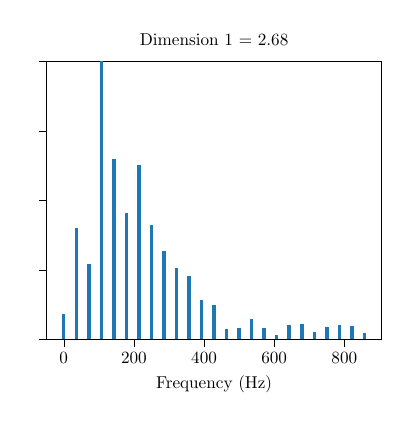
\begin{tikzpicture}[scale=0.62]

\definecolor{darkgray176}{RGB}{176,176,176}
\definecolor{steelblue31119180}{RGB}{31,119,180}

\begin{axis}[
yticklabel={\empty},
tick align=outside,
tick pos=left,
x grid style={darkgray176},
xlabel={Frequency (Hz)},
xmin=-48.3571428571429, xmax=905.5,
xtick style={color=black},
y grid style={darkgray176},
%ylabel={Magnitude},
ymin=0, ymax=4,
title={Dimension 1 = 2.68},
ytick style={color=black}
]
\draw[draw=none,fill=steelblue31119180] (axis cs:-5,0) rectangle (axis cs:5,0.363293109461665);
\draw[draw=none,fill=steelblue31119180] (axis cs:30.7142857142857,0) rectangle (axis cs:40.7142857142857,1.59671692845371);
\draw[draw=none,fill=steelblue31119180] (axis cs:66.4285714285714,0) rectangle (axis cs:76.4285714285714,1.08375129075336);
\draw[draw=none,fill=steelblue31119180] (axis cs:102.142857142857,0) rectangle (axis cs:112.142857142857,5.72028640718505);
\draw[draw=none,fill=steelblue31119180] (axis cs:137.857142857143,0) rectangle (axis cs:147.857142857143,2.60109171070077);
\draw[draw=none,fill=steelblue31119180] (axis cs:173.571428571429,0) rectangle (axis cs:183.571428571429,1.82230187959835);
\draw[draw=none,fill=steelblue31119180] (axis cs:209.285714285714,0) rectangle (axis cs:219.285714285714,2.50466396839656);
\draw[draw=none,fill=steelblue31119180] (axis cs:245,0) rectangle (axis cs:255,1.64154431128106);
\draw[draw=none,fill=steelblue31119180] (axis cs:280.714285714286,0) rectangle (axis cs:290.714285714286,1.2779936763853);
\draw[draw=none,fill=steelblue31119180] (axis cs:316.428571428571,0) rectangle (axis cs:326.428571428571,1.02566988726104);
\draw[draw=none,fill=steelblue31119180] (axis cs:352.142857142857,0) rectangle (axis cs:362.142857142857,0.906444113984638);
\draw[draw=none,fill=steelblue31119180] (axis cs:387.857142857143,0) rectangle (axis cs:397.857142857143,0.567573738688084);
\draw[draw=none,fill=steelblue31119180] (axis cs:423.571428571429,0) rectangle (axis cs:433.571428571429,0.497884322563813);
\draw[draw=none,fill=steelblue31119180] (axis cs:459.285714285714,0) rectangle (axis cs:469.285714285714,0.143370970638671);
\draw[draw=none,fill=steelblue31119180] (axis cs:495,0) rectangle (axis cs:505,0.158030205491621);
\draw[draw=none,fill=steelblue31119180] (axis cs:530.714285714286,0) rectangle (axis cs:540.714285714286,0.287791882784369);
\draw[draw=none,fill=steelblue31119180] (axis cs:566.428571428571,0) rectangle (axis cs:576.428571428571,0.164560600100172);
\draw[draw=none,fill=steelblue31119180] (axis cs:602.142857142857,0) rectangle (axis cs:612.142857142857,0.0653538748355305);
\draw[draw=none,fill=steelblue31119180] (axis cs:637.857142857143,0) rectangle (axis cs:647.857142857143,0.209706204538538);
\draw[draw=none,fill=steelblue31119180] (axis cs:673.571428571429,0) rectangle (axis cs:683.571428571429,0.216581742305538);
\draw[draw=none,fill=steelblue31119180] (axis cs:709.285714285714,0) rectangle (axis cs:719.285714285714,0.104565114650486);
\draw[draw=none,fill=steelblue31119180] (axis cs:745,0) rectangle (axis cs:755,0.18370350932939);
\draw[draw=none,fill=steelblue31119180] (axis cs:780.714285714286,0) rectangle (axis cs:790.714285714286,0.206670350113575);
\draw[draw=none,fill=steelblue31119180] (axis cs:816.428571428571,0) rectangle (axis cs:826.428571428571,0.196489132073225);
\draw[draw=none,fill=steelblue31119180] (axis cs:852.142857142857,0) rectangle (axis cs:862.142857142857,0.0885177801919891);
\end{axis}

\end{tikzpicture}

	\end{subfigure}
	
	\caption{The first dimension is being modified, while other dimensions are fixed at 0. The dimension has influence on the 150Hz frequency band, but also neighbouring ranges.}
	\label{fig:interpol_dim1}
\end{figure}


% one dimension
\begin{figure}
	\centering
	\begin{subfigure}{0.34\textwidth}
		\centering
		% This file was created with tikzplotlib v0.10.1.
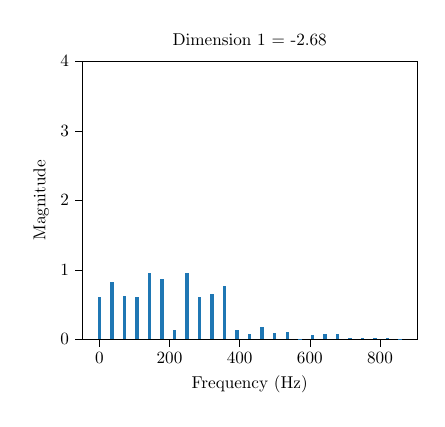
\begin{tikzpicture}[scale=0.62]

\definecolor{darkgray176}{RGB}{176,176,176}
\definecolor{steelblue31119180}{RGB}{31,119,180}

\begin{axis}[
tick align=outside,
tick pos=left,
x grid style={darkgray176},
xlabel={Frequency (Hz)},
xmin=-48.3571428571429, xmax=905.5,
xtick style={color=black},
y grid style={darkgray176},
ylabel={Magnitude},
ymin=0, ymax=4,
title={Dimension 1 = -2.68},
ytick style={color=black}
]
\draw[draw=none,fill=steelblue31119180] (axis cs:-5,0) rectangle (axis cs:5,0.605088098905981);
\draw[draw=none,fill=steelblue31119180] (axis cs:30.7142857142857,0) rectangle (axis cs:40.7142857142857,0.824946037495217);
\draw[draw=none,fill=steelblue31119180] (axis cs:66.4285714285714,0) rectangle (axis cs:76.4285714285714,0.618337924452538);
\draw[draw=none,fill=steelblue31119180] (axis cs:102.142857142857,0) rectangle (axis cs:112.142857142857,0.606547406467815);
\draw[draw=none,fill=steelblue31119180] (axis cs:137.857142857143,0) rectangle (axis cs:147.857142857143,0.952736687378679);
\draw[draw=none,fill=steelblue31119180] (axis cs:173.571428571429,0) rectangle (axis cs:183.571428571429,0.867459344161617);
\draw[draw=none,fill=steelblue31119180] (axis cs:209.285714285714,0) rectangle (axis cs:219.285714285714,0.142171590262196);
\draw[draw=none,fill=steelblue31119180] (axis cs:245,0) rectangle (axis cs:255,0.959357311317153);
\draw[draw=none,fill=steelblue31119180] (axis cs:280.714285714286,0) rectangle (axis cs:290.714285714286,0.614147542320182);
\draw[draw=none,fill=steelblue31119180] (axis cs:316.428571428571,0) rectangle (axis cs:326.428571428571,0.651510920840633);
\draw[draw=none,fill=steelblue31119180] (axis cs:352.142857142857,0) rectangle (axis cs:362.142857142857,0.767848611698322);
\draw[draw=none,fill=steelblue31119180] (axis cs:387.857142857143,0) rectangle (axis cs:397.857142857143,0.130737421425031);
\draw[draw=none,fill=steelblue31119180] (axis cs:423.571428571429,0) rectangle (axis cs:433.571428571429,0.0781024768115382);
\draw[draw=none,fill=steelblue31119180] (axis cs:459.285714285714,0) rectangle (axis cs:469.285714285714,0.174989028847861);
\draw[draw=none,fill=steelblue31119180] (axis cs:495,0) rectangle (axis cs:505,0.0957224281064073);
\draw[draw=none,fill=steelblue31119180] (axis cs:530.714285714286,0) rectangle (axis cs:540.714285714286,0.105812453640171);
\draw[draw=none,fill=steelblue31119180] (axis cs:566.428571428571,0) rectangle (axis cs:576.428571428571,0.00668246230492007);
\draw[draw=none,fill=steelblue31119180] (axis cs:602.142857142857,0) rectangle (axis cs:612.142857142857,0.0584750394429784);
\draw[draw=none,fill=steelblue31119180] (axis cs:637.857142857143,0) rectangle (axis cs:647.857142857143,0.0829703251371982);
\draw[draw=none,fill=steelblue31119180] (axis cs:673.571428571429,0) rectangle (axis cs:683.571428571429,0.0786316144734407);
\draw[draw=none,fill=steelblue31119180] (axis cs:709.285714285714,0) rectangle (axis cs:719.285714285714,0.0183265263662661);
\draw[draw=none,fill=steelblue31119180] (axis cs:745,0) rectangle (axis cs:755,0.0136594016374186);
\draw[draw=none,fill=steelblue31119180] (axis cs:780.714285714286,0) rectangle (axis cs:790.714285714286,0.0150421133154433);
\draw[draw=none,fill=steelblue31119180] (axis cs:816.428571428571,0) rectangle (axis cs:826.428571428571,0.0199113615327003);
\draw[draw=none,fill=steelblue31119180] (axis cs:852.142857142857,0) rectangle (axis cs:862.142857142857,0.00824199961136327);
\end{axis}

\end{tikzpicture}

	\end{subfigure}\hfill
	\begin{subfigure}{0.3\textwidth}
		\centering
		% This file was created with tikzplotlib v0.10.1.
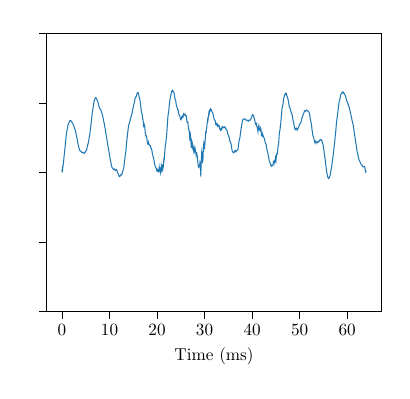
\begin{tikzpicture}[scale=0.62]

\definecolor{darkgray176}{RGB}{176,176,176}
\definecolor{steelblue31119180}{RGB}{31,119,180}

\begin{axis}[
yticklabel={\empty},
tick align=outside,
tick pos=left,
x grid style={darkgray176},
xlabel={Time (ms)},
xmin=-3.2, xmax=67.2,
xtick style={color=black},
y grid style={darkgray176},
% ylabel={Amplitude},
% ymin=-0.15, ymax=0.15,
ymin=-0.1, ymax=0.1,
ytick style={color=black}
]
\addplot [semithick, steelblue31119180]
table {%
0 0
0.0625610948191593 0.00267421979664707
0.125122189638319 0.00195263445792485
0.187683284457478 0.00448575329658223
0.250244379276637 0.00506307051416017
0.312805474095797 0.00741872769886972
0.375366568914956 0.00896099196129705
0.437927663734115 0.0115803680341702
0.500488758553275 0.0133900876509304
0.563049853372434 0.0151754755341063
0.625610948191593 0.0175304286389494
0.688172043010753 0.0195827149455586
0.750733137829912 0.0220035516719752
0.813294232649071 0.0241572310672827
0.875855327468231 0.0260075675241671
0.93841642228739 0.0276190532682753
1.00097751710655 0.029011056083869
1.06353861192571 0.0303319803605681
1.12609970674487 0.0314772311226626
1.18866080156403 0.0323503866813574
1.25122189638319 0.0340090383259345
1.31378299120235 0.0342868589673224
1.37634408602151 0.034962264941104
1.43890518084066 0.0355454103753539
1.50146627565982 0.0360117456070052
1.56402737047898 0.0365307936963797
1.62658846529814 0.0370469956639663
1.6891495601173 0.0372855405697375
1.75171065493646 0.0373638160362883
1.81427174975562 0.0371841114243804
1.87683284457478 0.0371509336557818
1.93939393939394 0.0367688526484099
2.0019550342131 0.0364753106155616
2.06451612903226 0.0361838696464416
2.12707722385142 0.0359691435804378
2.18963831867058 0.0355138606187011
2.25219941348974 0.0352915312351981
2.3147605083089 0.0347998261102134
2.37732160312805 0.0344101194336005
2.43988269794721 0.0336631536920749
2.50244379276637 0.0331262272681571
2.56500488758553 0.0324098647864333
2.62756598240469 0.0318902237095004
2.69012707722385 0.0313611501975318
2.75268817204301 0.030779401080743
2.81524926686217 0.0301372612829257
2.87781036168133 0.0291732079745475
2.94037145650049 0.0278471793837386
3.00293255131965 0.026998937900159
3.06549364613881 0.0261555616457092
3.12805474095797 0.0251639858926059
3.19061583577713 0.0240808387786762
3.25317693059629 0.0226956488526374
3.31573802541544 0.0215881998074457
3.3782991202346 0.0205637725818454
3.44086021505376 0.0194245896512462
3.50342130987292 0.0185915641158907
3.56598240469208 0.0176511272853595
3.62854349951124 0.016837186412203
3.6911045943304 0.0160462343054783
3.75366568914956 0.0156823699676658
3.81622678396872 0.0154439510553638
3.87878787878788 0.0154666042124683
3.94134897360704 0.0152564826052734
4.0039100684262 0.0150434925245487
4.06647116324536 0.01496300729445
4.12903225806452 0.0145273268102638
4.19159335288368 0.0143023412947781
4.25415444770283 0.0141885221670887
4.31671554252199 0.0143579145090496
4.37927663734115 0.0143627272509148
4.44183773216031 0.0143107777445023
4.50439882697947 0.0143003093455631
4.56695992179863 0.0140994674365017
4.62952101661779 0.0139923333422529
4.69208211143695 0.0136977836183788
4.75464320625611 0.013858715826072
4.81720430107527 0.0140708540115626
4.87976539589443 0.0146523808071778
4.94232649071359 0.0149836221114456
5.00488758553275 0.0151687482169821
5.06744868035191 0.0155991362598984
5.13000977517107 0.0159412591371281
5.19257086999022 0.0162529259035227
5.25513196480938 0.017360441337539
5.31769305962854 0.0182014699926999
5.3802541544477 0.0193291187581341
5.44281524926686 0.0200854901912625
5.50537634408602 0.0208316617795537
5.56793743890518 0.0217071624084914
5.63049853372434 0.0229126865049698
5.6930596285435 0.0242266035106175
5.75562072336266 0.0256323526474126
5.81818181818182 0.0267178274013779
5.88074291300098 0.0283921178146279
5.94330400782014 0.0298888944198659
6.0058651026393 0.0314556878562634
6.06842619745846 0.0335125506820042
6.13098729227761 0.0353603800185178
6.19354838709677 0.0371862264169801
6.25610948191593 0.0392754322130921
6.31867057673509 0.0411166230822938
6.38123167155425 0.0428521498174699
6.44379276637341 0.0441375720776246
6.50635386119257 0.0457053787929834
6.56891495601173 0.0472871441710904
6.63147605083089 0.048761960190019
6.69403714565005 0.0498478819788201
6.75659824046921 0.050987220705211
6.81915933528837 0.0516526354504121
6.88172043010753 0.052490993072429
6.94428152492669 0.0530063456738275
7.00684261974585 0.0534649434775289
7.069403714565 0.0537074036634038
7.13196480938416 0.0537072170656885
7.19452590420332 0.0535349667596677
7.25708699902248 0.0530148078673833
7.31964809384164 0.0528068320274003
7.3822091886608 0.0521574912434362
7.44477028347996 0.0515556330096162
7.50733137829912 0.0511457352595857
7.56989247311828 0.0503554332160181
7.63245356793744 0.0496244228928407
7.6950146627566 0.0487227421199297
7.75757575757576 0.0479266882281412
7.82013685239492 0.0471831423031095
7.88269794721408 0.046654381715526
7.94525904203324 0.0460351152001413
8.00782013685239 0.0457550140146898
8.07038123167155 0.0454348212550462
8.13294232649071 0.0452133226112798
8.19550342130987 0.0445972337685198
8.25806451612903 0.0439055550603136
8.32062561094819 0.0433501996252893
8.38318670576735 0.0427576806942476
8.44574780058651 0.0420135908768324
8.50830889540567 0.0413939108542246
8.57086999022483 0.040383708649629
8.63343108504399 0.0394220507029127
8.69599217986315 0.0382373149225439
8.75855327468231 0.0370243414417128
8.82111436950147 0.0361064742824549
8.88367546432062 0.0353182733026156
8.94623655913978 0.034049863776853
9.00879765395894 0.0328304045656122
9.0713587487781 0.0317752120300822
9.13391984359726 0.0303793267955965
9.19648093841642 0.0287503501471361
9.25904203323558 0.0277123870792364
9.32160312805474 0.0264058492072691
9.3841642228739 0.0252075347437624
9.44672531769306 0.0238300412674803
9.50928641251222 0.0225178186025176
9.57184750733138 0.0210519984932589
9.63440860215054 0.0198594470538439
9.6969696969697 0.0187120908363299
9.75953079178886 0.0173988586176962
9.82209188660802 0.0162397695983872
9.88465298142718 0.0150185930283188
9.94721407624633 0.0135728019423499
10.0097751710655 0.0123385272515921
10.0723362658847 0.0110240861762566
10.1348973607038 0.00961095098504398
10.197458455523 0.00825266510554073
10.2600195503421 0.0075971999443259
10.3225806451613 0.00651535481935547
10.3851417399804 0.00549221840684365
10.4477028347996 0.00441473745945787
10.5102639296188 0.00380801213386297
10.5728250244379 0.00333096788884782
10.6353861192571 0.0030224520516448
10.6979472140762 0.00274330640315485
10.7605083088954 0.00251342399357176
10.8230694037146 0.00208306508657695
10.8856304985337 0.00217947526630069
10.9481915933529 0.00227255503649761
11.010752688172 0.00244182444387867
11.0733137829912 0.00224105331533291
11.1358748778104 0.00175680994681599
11.1984359726295 0.00137892175367501
11.2609970674487 0.0013601645838218
11.3235581622678 0.001649708713779
11.386119257087 0.00193779625522951
11.4486803519062 0.00198972274349931
11.5112414467253 0.00166785174057631
11.5738025415445 0.00142994691833548
11.6363636363636 0.00061140903695063
11.6989247311828 -0.000307942650491191
11.761485826002 -0.000503915605132532
11.8240469208211 -0.00113124737401337
11.8866080156403 -0.00155196709236092
11.9491691104594 -0.00214502619049591
12.0117302052786 -0.00279614021264213
12.0742913000978 -0.00304161296212429
12.1368523949169 -0.00297893156076282
12.1994134897361 -0.00285662688817447
12.2619745845552 -0.00236801814582865
12.3245356793744 -0.0021942504504122
12.3870967741935 -0.00160614665477507
12.4496578690127 -0.00156108215123502
12.5122189638319 -0.0018311939707512
12.574780058651 -0.00173706366869012
12.6373411534702 -0.000912511972519309
12.6999022482893 -0.000196902665836721
12.7624633431085 0.000736978850013351
12.8250244379277 0.00106108622335968
12.8875855327468 0.00214182240806542
12.950146627566 0.00270913908383713
13.0127077223851 0.00340024156829129
13.0752688172043 0.00556807706673299
13.1378299120235 0.00725564627725183
13.2003910068426 0.00904701511400187
13.2629521016618 0.0112418273021399
13.3255131964809 0.0124709883655621
13.3880742913001 0.0139866596431938
13.4506353861193 0.0154722398884398
13.5131964809384 0.0179199806613919
13.5757575757576 0.0204215760935437
13.6383186705767 0.0226809065843607
13.7008797653959 0.0248251628578583
13.7634408602151 0.0266148869789416
13.8260019550342 0.0284216282261082
13.8885630498534 0.0303372205931508
13.9511241446725 0.0320307074273087
14.0136852394917 0.0336226689249627
14.0762463343109 0.0342720239436871
14.13880742913 0.0349491323751351
14.2013685239492 0.0356921560931241
14.2639296187683 0.0364141654485394
14.3264907135875 0.0373742953598325
14.3890518084066 0.0380467732554394
14.4516129032258 0.0389382684182736
14.514173998045 0.039927060713123
14.5767350928641 0.0404909389459493
14.6392961876833 0.0411950073032872
14.7018572825024 0.0419001485442311
14.7644183773216 0.0429625525753781
14.8269794721408 0.0438603695558488
14.8895405669599 0.0452642597727849
14.9521016617791 0.0463684541105001
15.0146627565982 0.0474161693220002
15.0772238514174 0.0484258940230367
15.1397849462366 0.048982958699907
15.2023460410557 0.0497803344033506
15.2649071358749 0.051131768807594
15.327468230694 0.0521033428106839
15.3900293255132 0.0531876813511083
15.4525904203324 0.0538189128325307
15.5151515151515 0.0541310210458257
15.5777126099707 0.0543522023735158
15.6402737047898 0.0549303894463785
15.702834799609 0.0555825384328267
15.7653958944282 0.0564133933201826
15.8279569892473 0.056831538196533
15.8905180840665 0.0572587951329534
15.9530791788856 0.057280189141937
16.0156402737048 0.0573616571822736
16.0782013685239 0.056989228402065
16.1407624633431 0.0559466459741952
16.2033235581623 0.0549218033787267
16.2658846529814 0.0539930620970876
16.3284457478006 0.0531750289925382
16.3910068426197 0.0521099569871366
16.4535679374389 0.0510703175386026
16.5161290322581 0.0493302415575712
16.5786901270772 0.0474945895286424
16.6412512218964 0.0456468005039213
16.7038123167155 0.0437111058040274
16.7663734115347 0.0426618811835554
16.8289345063539 0.0419866980607908
16.891495601173 0.0413465699197348
16.9540566959922 0.0398208843953798
17.0166177908113 0.0385363369120443
17.0791788856305 0.0372270050723532
17.1417399804497 0.0345423184062117
17.2043010752688 0.032461166021324
17.266862170088 0.0347551361239813
17.3294232649071 0.0341661413175619
17.3919843597263 0.0338865765739134
17.4545454545455 0.0314861332828348
17.5171065493646 0.0286533663273295
17.5796676441838 0.0271085365361307
17.6422287390029 0.0262852582228411
17.7047898338221 0.0263691197621945
17.7673509286412 0.0262591917002219
17.8299120234604 0.0251460206091317
17.8924731182796 0.023419109804015
17.9550342130987 0.0213664465766848
18.0175953079179 0.0208063320833043
18.080156402737 0.0203971048855275
18.1427174975562 0.0208537711262091
18.2052785923754 0.0216071604644536
18.2678396871945 0.020109887729205
18.3304007820137 0.0199684586124686
18.3929618768328 0.0197349161051673
18.455522971652 0.0194785226671752
18.5180840664712 0.0194128193889807
18.5806451612903 0.0193844509701575
18.6432062561095 0.0188214922176341
18.7057673509286 0.0173547650001878
18.7683284457478 0.0172885383187064
18.830889540567 0.0166502374325417
18.8934506353861 0.0162434242228783
18.9560117302053 0.0150629650757722
19.0185728250244 0.013391328265459
19.0811339198436 0.0127082065490683
19.1436950146628 0.0115744774434661
19.2062561094819 0.0109363535085906
19.2688172043011 0.0104743799254779
19.3313782991202 0.00898958691272917
19.3939393939394 0.00790707682344046
19.4565004887586 0.0066469337168502
19.5190615835777 0.00564898771733657
19.5816226783969 0.0047800187185363
19.644183773216 0.00409872611968224
19.7067448680352 0.00366864474681465
19.7693059628544 0.00332232838895314
19.8318670576735 0.00288059430803197
19.8944281524927 0.00273982084238809
19.9569892473118 0.000845879196159301
20.019550342131 0.000760033273321092
20.0821114369501 0.00095205489120001
20.1446725317693 0.0019063416846599
20.2072336265885 0.00162790942926211
20.2697947214076 0.000875847490608168
20.3323558162268 0.000575767573286014
20.3949169110459 0.00160671152786251
20.4574780058651 0.00388647337332149
20.5200391006843 0.00233205468489453
20.5826001955034 0.00152916488540837
20.6451612903226 0.00328123563479993
20.7077223851417 0.00326864568303582
20.7702834799609 -0.00020999720325568
20.8328445747801 0.000763068778598764
20.8954056695992 0.00438050786442945
20.9579667644184 0.0029384327555332
21.0205278592375 0.000206796255760179
21.0830889540567 0.00278985447351359
21.1456500488759 0.00508365880075263
21.208211143695 0.00488976083280753
21.2707722385142 0.00338998097718811
21.3333333333333 0.00464094616472721
21.3958944281525 0.00786668587683582
21.4584555229717 0.0097706981789856
21.5210166177908 0.00937353533384038
21.58357771261 0.0119085969113884
21.6461388074291 0.0154543465107155
21.7086999022483 0.0183054468160238
21.7712609970674 0.0201115640770655
21.8338220918866 0.0206162288205977
21.8963831867058 0.0229037094675551
21.9589442815249 0.0247902948616886
22.0215053763441 0.0266693644826451
22.0840664711632 0.030081022257679
22.1466275659824 0.0328973525659867
22.2091886608016 0.0361175192438088
22.2717497556207 0.0395221697477913
22.3343108504399 0.041304173204731
22.396871945259 0.0427716355006104
22.4594330400782 0.0439727842436333
22.5219941348974 0.04629844911615
22.5845552297165 0.0490542658088494
22.6471163245357 0.0508796651724759
22.7096774193548 0.0520982259223538
22.772238514174 0.0532420461729737
22.8347996089932 0.0545685695609914
22.8973607038123 0.0551733477560044
22.9599217986315 0.0559879976305619
23.0224828934506 0.0578949249723702
23.0850439882698 0.0583804640755101
23.147605083089 0.0584930904439031
23.2101661779081 0.0588970233377648
23.2727272727273 0.0583844416859475
23.3352883675464 0.0586766382225972
23.3978494623656 0.0583387540593263
23.4604105571848 0.0581928974350701
23.5229716520039 0.0575271020438577
23.5855327468231 0.0569285704942742
23.6480938416422 0.0559307399787599
23.7106549364614 0.0543003477199861
23.7732160312805 0.0534002241184198
23.8357771260997 0.0520780251260377
23.8983382209189 0.0516900767864457
23.960899315738 0.0508313895888692
24.0234604105572 0.049175866521742
24.0860215053763 0.0479400197584783
24.1485826001955 0.0473373903895665
24.2111436950147 0.046511578878874
24.2737047898338 0.0462514713264543
24.336265884653 0.0451448697848054
24.3988269794721 0.0451817311991083
24.4613880742913 0.0443530065114023
24.5239491691105 0.0426578202784673
24.5865102639296 0.0416546216196329
24.6490713587488 0.0413088361156389
24.7116324535679 0.041108225174576
24.7741935483871 0.0408650341654016
24.8367546432063 0.0398515648812143
24.8993157380254 0.038847956440447
24.9618768328446 0.0380346358281252
25.0244379276637 0.0378304746854078
25.0869990224829 0.0382387661689188
25.1495601173021 0.0390100164114992
25.2121212121212 0.0399538556283171
25.2746823069404 0.040413034577305
25.3372434017595 0.0400065938966715
25.3998044965787 0.0394734188400843
25.4623655913978 0.0394740778832666
25.524926686217 0.0411028750513918
25.5874877810362 0.0420756560485384
25.6500488758553 0.0417780720757162
25.7126099706745 0.0412677814774324
25.7751710654936 0.041175230032057
25.8377321603128 0.0413646532599527
25.900293255132 0.0417800190697405
25.9628543499511 0.0412614583269941
26.0254154447703 0.0406542915544989
26.0879765395894 0.0408050164667742
26.1505376344086 0.0405792076621325
26.2130987292278 0.0390043036023543
26.2756598240469 0.0368666124866068
26.3382209188661 0.0360929401389315
26.4007820136852 0.0362097313818781
26.4633431085044 0.036331480986212
26.5259042033236 0.0345905183860896
26.5884652981427 0.031986461903168
26.6510263929619 0.031094742556515
26.713587487781 0.0309626471546214
26.7761485826002 0.0293936625811274
26.8387096774194 0.0263035376706431
26.9012707722385 0.0239715223744118
26.9638318670577 0.0245473122229674
27.0263929618768 0.026747274624943
27.088954056696 0.0248879576893933
27.1515151515152 0.0209304007955573
27.2140762463343 0.0176937769814408
27.2766373411535 0.0196157470454743
27.3391984359726 0.0221516430880492
27.4017595307918 0.0213706412317117
27.4643206256109 0.0188635372914527
27.5268817204301 0.0167689943505872
27.5894428152493 0.0163053760518077
27.6520039100684 0.0177176835621732
27.7145650048876 0.0165713070960076
27.7771260997067 0.0141103166617082
27.8396871945259 0.0146560471428454
27.9022482893451 0.0159809314031318
27.9648093841642 0.0179326702619403
28.0273704789834 0.0170464531690581
28.0899315738025 0.0151981798565982
28.1524926686217 0.0144559601349128
28.2150537634409 0.0127864169377473
28.27761485826 0.0140569939160627
28.3401759530792 0.0141271333486017
28.4027370478983 0.0123410444444488
28.4652981427175 0.0116867676508392
28.5278592375367 0.00907893372355493
28.5904203323558 0.00709933834013876
28.652981427175 0.00512608153816542
28.7155425219941 0.00378594341035113
28.7781036168133 0.00356751068050036
28.8406647116325 0.00437589089148555
28.9032258064516 0.00465376368693767
28.9657869012708 0.00537902522078357
29.0283479960899 0.00695361941506611
29.0909090909091 0.00594923797656189
29.1534701857282 0.0013902217881683
29.2160312805474 -0.00304396178496898
29.2785923753666 0.00566547975228154
29.3411534701857 0.0108653606896089
29.4037145650049 0.014694018147427
29.466275659824 0.0133876833037809
29.5288367546432 0.0101675867400736
29.5913978494624 0.00803752129356707
29.6539589442815 0.00901241266766776
29.7165200391007 0.0144135524133696
29.7790811339198 0.0189351138667015
29.841642228739 0.0207817511103195
29.9042033235582 0.0193139174816545
29.9667644183773 0.0165541066113543
30.0293255131965 0.0189539923051323
30.0918866080156 0.0218169781491379
30.1544477028348 0.0246398184022421
30.217008797654 0.0282433863696465
30.2795698924731 0.0278777189913296
30.3421309872923 0.0289339464911617
30.4046920821114 0.0309737586632065
30.4672531769306 0.0327821483513302
30.5298142717498 0.0346808726039013
30.5923753665689 0.0366036100777363
30.6549364613881 0.0380971568562855
30.7174975562072 0.0375351592286591
30.7800586510264 0.0395417567124028
30.8426197458456 0.0406106800015721
30.9051808406647 0.0431468461276936
30.9677419354839 0.0440592289932313
31.030303030303 0.0431223926557736
31.0928641251222 0.044251091953072
31.1554252199413 0.044091906240128
31.2179863147605 0.0447321454734921
31.2805474095797 0.0457030936278119
31.3431085043988 0.0453781697494893
31.405669599218 0.0451644942153496
31.4682306940371 0.0443997886414227
31.5307917888563 0.0437652633369756
31.5933528836755 0.0434029524452176
31.6559139784946 0.043035791225491
31.7184750733138 0.0426897188741441
31.7810361681329 0.0420002157354722
31.8435972629521 0.0409411973268056
31.9061583577713 0.039571873412148
31.9687194525904 0.0386384047371202
32.0312805474096 0.0383785877573438
32.0938416422287 0.0375490882092557
32.1564027370479 0.0375753101944661
32.2189638318671 0.0374420748537412
32.2815249266862 0.0360706945788388
32.3440860215054 0.0350615131037851
32.4066471163245 0.0339929430507932
32.4692082111437 0.0340246002345491
32.5317693059629 0.0349592938636842
32.594330400782 0.0352224107842641
32.6568914956012 0.034789714257607
32.7194525904203 0.0336865213565812
32.7820136852395 0.0331596681176305
32.8445747800587 0.0334299338702932
32.9071358748778 0.0338081808875471
32.969696969697 0.033365224911408
33.0322580645161 0.0329333330474554
33.0948191593353 0.0332109972266508
33.1573802541544 0.0320883396838155
33.2199413489736 0.0309007317046266
33.2825024437928 0.0308718603716131
33.3450635386119 0.030459921162499
33.4076246334311 0.0313069512603307
33.4701857282502 0.0315470496121565
33.5327468230694 0.0310009366223627
33.5953079178886 0.0306450518563696
33.6578690127077 0.0318058445295892
33.7204301075269 0.0329603675392366
33.782991202346 0.0327633887562147
33.8455522971652 0.032416258422423
33.9081133919844 0.0322558210119387
33.9706744868035 0.0320788991918837
34.0332355816227 0.0323125378903318
34.0957966764418 0.0326428515973154
34.158357771261 0.0326298984297472
34.2209188660802 0.032318359519467
34.2834799608993 0.0326219256421076
34.3460410557185 0.0323100589062811
34.4086021505376 0.0318218369277254
34.4711632453568 0.0310809285082251
34.533724340176 0.0310058263226076
34.5962854349951 0.0309875087370096
34.6588465298143 0.0306313110466315
34.7214076246334 0.0300611066044775
34.7839687194526 0.0293552047379118
34.8465298142717 0.0284407946480509
34.9090909090909 0.0275458454747092
34.9716520039101 0.0268777255023505
35.0342130987292 0.0267992109508196
35.0967741935484 0.0259139400816733
35.1593352883675 0.0252057173592516
35.2218963831867 0.0244404716182314
35.2844574780059 0.0227533189738251
35.347018572825 0.0225678494751803
35.4095796676442 0.0221244483268506
35.4721407624633 0.0217717170190951
35.5347018572825 0.0210364933925902
35.5972629521017 0.0201191887521674
35.6598240469208 0.0188929513752286
35.72238514174 0.0170571037685591
35.7849462365591 0.0159716786396119
35.8475073313783 0.0150278387563931
35.9100684261975 0.01489631146127
35.9726295210166 0.0146592597305076
36.0351906158358 0.0141087751125485
36.0977517106549 0.014124936951308
36.1603128054741 0.014254863567847
36.2228739002933 0.0143559359483792
36.2854349951124 0.0151110854862897
36.3479960899316 0.0150740762566192
36.4105571847507 0.0157257782082316
36.4731182795699 0.0156458070681941
36.5356793743891 0.0150090577654388
36.5982404692082 0.0147384244052808
36.6608015640274 0.015120394850188
36.7233626588465 0.0154524166027734
36.7859237536657 0.0158782299892032
36.8484848484849 0.0158998847685077
36.911045943304 0.0161424008337371
36.9736070381232 0.0162015636984117
37.0361681329423 0.0167102424422405
37.0987292277615 0.0182204747960365
37.1612903225806 0.0200580241939714
37.2238514173998 0.0217561341133897
37.286412512219 0.0231641612652023
37.3489736070381 0.0238318093219373
37.4115347018573 0.0247525442883241
37.4740957966764 0.025644510700381
37.5366568914956 0.0275202778514879
37.5992179863148 0.0292770331534298
37.6617790811339 0.0308391401746318
37.7243401759531 0.0322980790063083
37.7869012707722 0.0334602463116482
37.8494623655914 0.0347619480904072
37.9120234604106 0.0359631676139457
37.9745845552297 0.0368996791847465
38.0371456500489 0.0378674757434738
38.099706744868 0.0381146148939636
38.1622678396872 0.0383059976245563
38.2248289345064 0.0384774612279232
38.2873900293255 0.0383171840049217
38.3499511241447 0.0384484256489361
38.4125122189638 0.0384597241212109
38.475073313783 0.0384790841216915
38.5376344086022 0.0383175552011498
38.6001955034213 0.0377998699016235
38.6627565982405 0.0377321959448612
38.7253176930596 0.0376487938124588
38.7878787878788 0.0376734474504536
38.8504398826979 0.0375150216967304
38.9130009775171 0.0375846544897888
38.9755620723363 0.0374904452902306
39.0381231671554 0.0374442960608128
39.1006842619746 0.0372936971420067
39.1632453567937 0.0369457174420269
39.2258064516129 0.0368236430710362
39.2883675464321 0.0373380606245697
39.3509286412512 0.0374558800476387
39.4134897360704 0.0376636466049641
39.4760508308895 0.0376178475528344
39.5386119257087 0.0375941767250775
39.6011730205279 0.0375067810814751
39.663734115347 0.0377316429959801
39.7262952101662 0.0381126951568287
39.7888563049853 0.0388838746188935
39.8514173998045 0.0394202564840268
39.9139784946237 0.0397456081043328
39.9765395894428 0.040315290339444
40.039100684262 0.0412298003457421
40.1016617790811 0.0414068146316537
40.1642228739003 0.0410492199574136
40.2267839687195 0.0411880649189271
40.2893450635386 0.0409462820694856
40.3519061583578 0.0401449904195374
40.4144672531769 0.0390465733406743
40.4770283479961 0.0386799932662343
40.5395894428152 0.0376865399668206
40.6021505376344 0.0366314517394189
40.6647116324536 0.0358175872347135
40.7272727272727 0.0348084318366918
40.7898338220919 0.0344157486531304
40.852394916911 0.0347675312081041
40.9149560117302 0.0350688882335977
40.9775171065494 0.0333061736634225
41.0400782013685 0.032600074356471
41.1026392961877 0.0321379145088434
41.1652003910068 0.0307046050080194
41.227761485826 0.0294969624176053
41.2903225806452 0.0325823667188806
41.3528836754643 0.0329074016895112
41.4154447702835 0.0337845209570836
41.4780058651026 0.0325840122975912
41.5405669599218 0.0306703675909738
41.603128054741 0.0305694714953298
41.6656891495601 0.030171353113223
41.7282502443793 0.031143564140954
41.7908113391984 0.0318894302554407
41.8533724340176 0.0306748176468782
41.9159335288368 0.0292985609669752
41.9784946236559 0.0267994198347292
42.0410557184751 0.0260753441394424
42.1036168132942 0.026039359364604
42.1661779081134 0.0267842792553549
42.2287390029325 0.0277295210439701
42.2913000977517 0.0265493077660236
42.3538611925709 0.0261299217016029
42.41642228739 0.0255084721661034
42.4789833822092 0.0248335181486921
42.5415444770283 0.0245418480742187
42.6041055718475 0.0241732470297918
42.6666666666667 0.0232807192951441
42.7292277614858 0.0216111164933338
42.791788856305 0.0214149535488873
42.8543499511241 0.0207516336130781
42.9169110459433 0.0204178342306194
42.9794721407625 0.0192357806592655
43.0420332355816 0.0175879018878307
43.1045943304008 0.0168795692693453
43.1671554252199 0.0155753857808466
43.2297165200391 0.0148914705776224
43.2922776148583 0.0144289083986426
43.3548387096774 0.0130980704580584
43.4173998044966 0.0120939013611012
43.4799608993157 0.0108472363548108
43.5425219941349 0.00960976536497692
43.6050830889541 0.00849363266809944
43.6676441837732 0.00765429090304284
43.7302052785924 0.00705099843245797
43.7927663734115 0.00663502100866037
43.8553274682307 0.00606322959283929
43.9178885630498 0.00568777587690836
43.980449657869 0.00445893265940576
44.0430107526882 0.00439443637526804
44.1055718475073 0.00446561516380031
44.1681329423265 0.00513564554368121
44.2306940371457 0.00521406070861823
44.2932551319648 0.00499794883462341
44.355816226784 0.00488837840051945
44.4183773216031 0.00564268229753216
44.4809384164223 0.00737928005366906
44.5434995112414 0.00707713632552155
44.6060606060606 0.0070919179442254
44.6686217008798 0.00851020454551992
44.7311827956989 0.00866406987751684
44.7937438905181 0.00704828820729361
44.8563049853372 0.00816068935953627
44.9188660801564 0.0108787558229962
44.9814271749756 0.010371167922824
45.0439882697947 0.00914865583618366
45.1065493646139 0.0114646889706336
45.169110459433 0.0132357996787406
45.2316715542522 0.0134156004817954
45.2942326490714 0.0132334446288711
45.3567937438905 0.0144499974472781
45.4193548387097 0.0173056817222987
45.4819159335288 0.019130442198639
45.544477028348 0.0196244097710792
45.6070381231672 0.021854941905244
45.6695992179863 0.025132772351596
45.7321603128055 0.0278786127168762
45.7947214076246 0.0295117591614248
45.8572825024438 0.0303778906852619
45.919843597263 0.0322564648426086
45.9824046920821 0.0339553831500217
46.0449657869013 0.0358612972128688
46.1075268817204 0.0385077691847278
46.1700879765396 0.0408807266175834
46.2326490713588 0.0432648152178508
46.2952101661779 0.0456662636709091
46.3577712609971 0.046847217615224
46.4203323558162 0.0477867429458763
46.4828934506354 0.0485950412004749
46.5454545454545 0.0505165232514793
46.6080156402737 0.0525513137322018
46.6705767350929 0.0537294811593735
46.733137829912 0.0543446789913513
46.7956989247312 0.0549502618490688
46.8582600195503 0.0558704715495235
46.9208211143695 0.0559133530329487
46.9833822091887 0.0559761648194706
47.0459433040078 0.0569916450940182
47.108504398827 0.0570250419883434
47.1710654936461 0.0568927230690319
47.2336265884653 0.056640900562236
47.2961876832845 0.0551848630653011
47.3587487781036 0.0547586485437634
47.4213098729228 0.0541026841936486
47.4838709677419 0.0536307193819554
47.5464320625611 0.0527246055135891
47.6089931573803 0.0517289356664479
47.6715542521994 0.0508142424545243
47.7341153470186 0.0493116723564713
47.7966764418377 0.0481130375179989
47.8592375366569 0.0468085671821473
47.9217986314761 0.0465829856202137
47.9843597262952 0.0462157163670685
48.0469208211144 0.0452095076736729
48.1094819159335 0.0442796264532025
48.1720430107527 0.0438324161955426
48.2346041055718 0.0430557673409188
48.297165200391 0.0426278280099728
48.3597262952102 0.0418391911711686
48.4222873900293 0.041594998058904
48.4848484848485 0.0406052067198537
48.5474095796676 0.0389845076664365
48.6099706744868 0.0375579707433751
48.672531769306 0.0365544479842847
48.7350928641251 0.0357116901280244
48.7976539589443 0.0348651324756596
48.8602150537634 0.0336367660953153
48.9227761485826 0.0324083252091649
48.9853372434018 0.0313928293670552
49.0478983382209 0.0309147811563046
49.1104594330401 0.030692954686992
49.1730205278592 0.0309709876699269
49.2355816226784 0.031597696648927
49.2981427174976 0.0318774469906896
49.3607038123167 0.0314093900085195
49.4232649071359 0.0308339031047223
49.485826001955 0.0304353637648118
49.5483870967742 0.031060064812341
49.6109481915934 0.0315283893490117
49.6735092864125 0.031664160946029
49.7360703812317 0.0318912170565198
49.7986314760508 0.0325307298582757
49.86119257087 0.0333566375601152
49.9237536656891 0.0340274055474752
49.9863147605083 0.0343475082337507
50.0488758553275 0.0348904801374219
50.1114369501466 0.0352367120098508
50.1739980449658 0.0354705928521684
50.2365591397849 0.0357889670037454
50.2991202346041 0.0362658038287481
50.3616813294233 0.0370228979681944
50.4242424242424 0.0380117535929788
50.4868035190616 0.0389377374933962
50.5493646138807 0.0395894841484922
50.6119257086999 0.0399620687244924
50.6744868035191 0.0408489817802595
50.7370478983382 0.0415870843897642
50.7996089931574 0.0421664896325544
50.8621700879765 0.0424486465118498
50.9247311827957 0.04317258929293
50.9872922776149 0.0436714500341772
51.049853372434 0.0439890157977594
51.1124144672532 0.044358433877006
51.1749755620723 0.0441271898738188
51.2375366568915 0.0438700103995737
51.3000977517107 0.0442643841985296
51.3626588465298 0.0446783232221331
51.425219941349 0.0449076517597059
51.4877810361681 0.0448242272755617
51.5503421309873 0.0448317967322477
51.6129032258064 0.0444544803711676
51.6754643206256 0.0442608096459307
51.7380254154448 0.0440060031816057
51.8005865102639 0.0440069565227217
51.8631476050831 0.0439781410690626
51.9257086999022 0.0437708097043013
51.9882697947214 0.0431585281082262
52.0508308895406 0.0425149987771277
52.1133919843597 0.0415439978023428
52.1759530791789 0.0401725728239569
52.238514173998 0.0387360111447024
52.3010752688172 0.0377038967825713
52.3636363636364 0.0366723598404364
52.4261974584555 0.0354431589950652
52.4887585532747 0.0341393890137896
52.5513196480938 0.0325012071730017
52.613880742913 0.0306788693315997
52.6764418377322 0.0291148989988475
52.7390029325513 0.0275694079686208
52.8015640273705 0.0265256427610812
52.8641251221896 0.0256399043680024
52.9266862170088 0.0253011354482856
52.989247311828 0.0243811560494284
53.0518084066471 0.0233437759894605
53.1143695014663 0.0225893578046927
53.1769305962854 0.0217172744632029
53.2394916911046 0.0211648024028697
53.3020527859238 0.0224554698717647
53.3646138807429 0.0222937956649013
53.4271749755621 0.0224200454199157
53.4897360703812 0.0216772929817176
53.5522971652004 0.0212178265189757
53.6148582600196 0.0211791725736385
53.6774193548387 0.0211344315039535
53.7399804496579 0.0214040229790721
53.802541544477 0.0220809991627145
53.8651026392962 0.0223197899376455
53.9276637341153 0.0223311759542423
53.9902248289345 0.0219567615943046
54.0527859237537 0.0220094107888923
54.1153470185728 0.0223439676015258
54.177908113392 0.0227976033185497
54.2404692082111 0.0232850162427097
54.3030303030303 0.0231732385741039
54.3655913978495 0.0234766053937135
54.4281524926686 0.0236280772266937
54.4907135874878 0.0235211834136692
54.5532746823069 0.0233881529639106
54.6158357771261 0.0231276766077514
54.6783968719453 0.0227126081547867
54.7409579667644 0.0217724376825119
54.8035190615836 0.0213462827656189
54.8660801564027 0.0205169620314651
54.9286412512219 0.020012508963079
54.9912023460411 0.0188231631359659
55.0537634408602 0.0171258385863996
55.1163245356794 0.0157880976828924
55.1788856304985 0.0139106013306862
55.2414467253177 0.0122885611727615
55.3040078201369 0.0112943628152882
55.366568914956 0.0093972099688221
55.4291300097752 0.00770373364413414
55.4916911045943 0.00584246838175831
55.5542521994135 0.00412534391425572
55.6168132942326 0.00245839351913796
55.6793743890518 0.000780038147771465
55.741935483871 -0.000622202431963335
55.8044965786901 -0.00163171173256339
55.8670576735093 -0.00270341847998656
55.9296187683284 -0.00340635501547468
55.9921798631476 -0.00384208765372503
56.0547409579668 -0.00413895264551961
56.1173020527859 -0.00444098088966786
56.1798631476051 -0.00418070636558568
56.2424242424242 -0.00360199775208126
56.3049853372434 -0.00304885953118549
56.3675464320626 -0.00252012568703495
56.4301075268817 -0.0017775341027206
56.4926686217009 -0.000825290630989413
56.55522971652 0.000563787831720022
56.6177908113392 0.00183773806040063
56.6803519061584 0.00313017317954221
56.7429130009775 0.00412363140049044
56.8054740957967 0.00566291729332415
56.8680351906158 0.00711228026628844
56.930596285435 0.0089067299181153
56.9931573802542 0.0104306080102746
57.0557184750733 0.0119805407827813
57.1182795698925 0.0143055500042054
57.1808406647116 0.0158458994674193
57.2434017595308 0.0175163397931458
57.3059628543499 0.0196888505309121
57.3685239491691 0.0215753390674979
57.4310850439883 0.023990589721112
57.4936461388074 0.0260414846317946
57.5562072336266 0.0279752023987844
57.6187683284457 0.0300400056807963
57.6813294232649 0.03277259705113
57.7438905180841 0.0352639255832193
57.8064516129032 0.0372064629749906
57.8690127077224 0.0387646770678308
57.9315738025415 0.0404650743154924
57.9941348973607 0.0420708640907342
58.0566959921799 0.0439263153711984
58.119257086999 0.0457073502526605
58.1818181818182 0.0474987526170232
58.2443792766373 0.0490374536392801
58.3069403714565 0.0505239223662622
58.3695014662757 0.0515297504136464
58.4320625610948 0.0522976404443777
58.494623655914 0.0528898979386976
58.5571847507331 0.0540614753273313
58.6197458455523 0.0552708644124944
58.6823069403715 0.0560077898302648
58.7448680351906 0.0564124975845087
58.8074291300098 0.0568147131195428
58.8699902248289 0.0571315971550005
58.9325513196481 0.0569640071871431
58.9951124144673 0.0570515101977632
59.0576735092864 0.0578324908986032
59.1202346041056 0.0576970315595701
59.1827956989247 0.057722884741041
59.2453567937439 0.0576931007119043
59.307917888563 0.0567069899596689
59.3704789833822 0.0566763006849897
59.4330400782014 0.05626079637306
59.4956011730205 0.0559517869348925
59.5581622678397 0.0556505410017069
59.6207233626588 0.055134919513006
59.683284457478 0.0544264769984568
59.7458455522972 0.053288635172365
59.8084066471163 0.0526271909202211
59.8709677419355 0.0517917160064943
59.9335288367546 0.0514830865479372
59.9960899315738 0.051134827451185
60.058651026393 0.0505215214002779
60.1212121212121 0.0497802963311022
60.1837732160313 0.0491487996876677
60.2463343108504 0.0484007759636973
60.3088954056696 0.0478875684631098
60.3714565004888 0.0473363406497362
60.4340175953079 0.0468872565710562
60.4965786901271 0.0460121147662314
60.5591397849462 0.0450108979618357
60.6217008797654 0.0438298725706042
60.6842619745846 0.0428822552430228
60.7468230694037 0.0419466333502024
60.8093841642229 0.0411196371971949
60.871945259042 0.0403209532504557
60.9345063538612 0.039276586408533
60.9970674486804 0.0380582447843817
61.0596285434995 0.0371007740639609
61.1221896383187 0.0360698294429835
61.1847507331378 0.0353156627153109
61.247311827957 0.0343963464181269
61.3098729227762 0.0335445323811511
61.3724340175953 0.031944404380762
61.4349951124145 0.0303682355849274
61.4975562072336 0.0286385904167317
61.5601173020528 0.0272719170461215
61.6226783968719 0.0258196607188395
61.6852394916911 0.0243035696796483
61.7478005865103 0.0227989208696088
61.8103616813294 0.021500640103588
61.8729227761486 0.0203646199444522
61.9354838709677 0.0187503377035741
61.9980449657869 0.0170625145069141
62.0606060606061 0.0159145622429523
62.1231671554252 0.0145981244120168
62.1857282502444 0.0137994386026324
62.2482893450635 0.012727528826888
62.3108504398827 0.0117746551146955
62.3734115347019 0.0107542865928754
62.435972629521 0.00994687242832177
62.4985337243402 0.00900293568755525
62.5610948191593 0.00859378858351987
62.6236559139785 0.00813819083475298
62.6862170087977 0.00771863340697855
62.7487781036168 0.00717838961205
62.811339198436 0.00671188235064406
62.8739002932551 0.00621034618456168
62.9364613880743 0.00593350649076647
62.9990224828935 0.0054801793064365
63.0615835777126 0.00537889578060146
63.1241446725318 0.00507545192613979
63.1867057673509 0.0048174845529966
63.2492668621701 0.00437471670401761
63.3118279569892 0.00417060399007413
63.3743890518084 0.00395582949529645
63.4369501466276 0.00400284605095289
63.4995112414467 0.00400681501456544
63.5620723362659 0.00419773767180632
63.624633431085 0.00398296317702864
63.6871945259042 0.00392700898354529
63.7497556207234 0.0032044941848936
63.8123167155425 0.00166316802922057
63.8748778103617 0.000470869909545896
63.9374389051808 0.000761237328659056
64 0
};
\end{axis}

\end{tikzpicture}

	\end{subfigure}\hfill
	\begin{subfigure}{0.3\textwidth}
		\centering
		% This file was created with tikzplotlib v0.10.1.
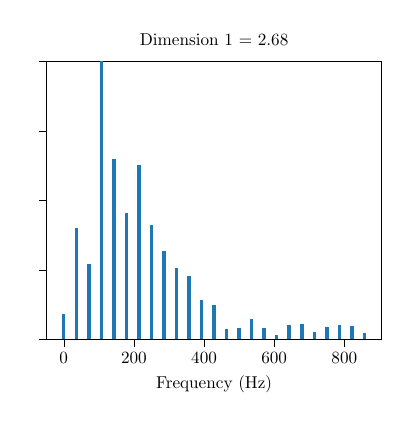
\begin{tikzpicture}[scale=0.62]

\definecolor{darkgray176}{RGB}{176,176,176}
\definecolor{steelblue31119180}{RGB}{31,119,180}

\begin{axis}[
yticklabel={\empty},
tick align=outside,
tick pos=left,
x grid style={darkgray176},
xlabel={Frequency (Hz)},
xmin=-48.3571428571429, xmax=905.5,
xtick style={color=black},
y grid style={darkgray176},
%ylabel={Magnitude},
ymin=0, ymax=4,
title={Dimension 1 = 2.68},
ytick style={color=black}
]
\draw[draw=none,fill=steelblue31119180] (axis cs:-5,0) rectangle (axis cs:5,0.363293109461665);
\draw[draw=none,fill=steelblue31119180] (axis cs:30.7142857142857,0) rectangle (axis cs:40.7142857142857,1.59671692845371);
\draw[draw=none,fill=steelblue31119180] (axis cs:66.4285714285714,0) rectangle (axis cs:76.4285714285714,1.08375129075336);
\draw[draw=none,fill=steelblue31119180] (axis cs:102.142857142857,0) rectangle (axis cs:112.142857142857,5.72028640718505);
\draw[draw=none,fill=steelblue31119180] (axis cs:137.857142857143,0) rectangle (axis cs:147.857142857143,2.60109171070077);
\draw[draw=none,fill=steelblue31119180] (axis cs:173.571428571429,0) rectangle (axis cs:183.571428571429,1.82230187959835);
\draw[draw=none,fill=steelblue31119180] (axis cs:209.285714285714,0) rectangle (axis cs:219.285714285714,2.50466396839656);
\draw[draw=none,fill=steelblue31119180] (axis cs:245,0) rectangle (axis cs:255,1.64154431128106);
\draw[draw=none,fill=steelblue31119180] (axis cs:280.714285714286,0) rectangle (axis cs:290.714285714286,1.2779936763853);
\draw[draw=none,fill=steelblue31119180] (axis cs:316.428571428571,0) rectangle (axis cs:326.428571428571,1.02566988726104);
\draw[draw=none,fill=steelblue31119180] (axis cs:352.142857142857,0) rectangle (axis cs:362.142857142857,0.906444113984638);
\draw[draw=none,fill=steelblue31119180] (axis cs:387.857142857143,0) rectangle (axis cs:397.857142857143,0.567573738688084);
\draw[draw=none,fill=steelblue31119180] (axis cs:423.571428571429,0) rectangle (axis cs:433.571428571429,0.497884322563813);
\draw[draw=none,fill=steelblue31119180] (axis cs:459.285714285714,0) rectangle (axis cs:469.285714285714,0.143370970638671);
\draw[draw=none,fill=steelblue31119180] (axis cs:495,0) rectangle (axis cs:505,0.158030205491621);
\draw[draw=none,fill=steelblue31119180] (axis cs:530.714285714286,0) rectangle (axis cs:540.714285714286,0.287791882784369);
\draw[draw=none,fill=steelblue31119180] (axis cs:566.428571428571,0) rectangle (axis cs:576.428571428571,0.164560600100172);
\draw[draw=none,fill=steelblue31119180] (axis cs:602.142857142857,0) rectangle (axis cs:612.142857142857,0.0653538748355305);
\draw[draw=none,fill=steelblue31119180] (axis cs:637.857142857143,0) rectangle (axis cs:647.857142857143,0.209706204538538);
\draw[draw=none,fill=steelblue31119180] (axis cs:673.571428571429,0) rectangle (axis cs:683.571428571429,0.216581742305538);
\draw[draw=none,fill=steelblue31119180] (axis cs:709.285714285714,0) rectangle (axis cs:719.285714285714,0.104565114650486);
\draw[draw=none,fill=steelblue31119180] (axis cs:745,0) rectangle (axis cs:755,0.18370350932939);
\draw[draw=none,fill=steelblue31119180] (axis cs:780.714285714286,0) rectangle (axis cs:790.714285714286,0.206670350113575);
\draw[draw=none,fill=steelblue31119180] (axis cs:816.428571428571,0) rectangle (axis cs:826.428571428571,0.196489132073225);
\draw[draw=none,fill=steelblue31119180] (axis cs:852.142857142857,0) rectangle (axis cs:862.142857142857,0.0885177801919891);
\end{axis}

\end{tikzpicture}

	\end{subfigure}
	
	\vspace{0.5cm} % Adjust vertical spacing between rows
	
	\begin{subfigure}{0.36\textwidth}
		\centering
		% This file was created with tikzplotlib v0.10.1.
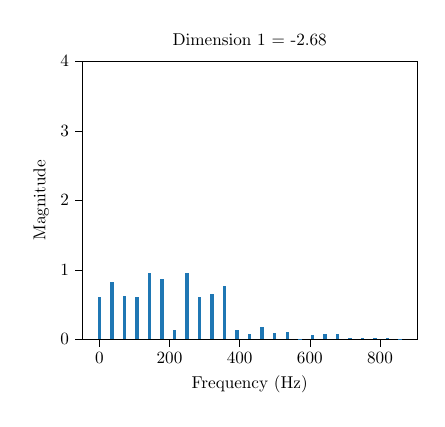
\begin{tikzpicture}[scale=0.62]

\definecolor{darkgray176}{RGB}{176,176,176}
\definecolor{steelblue31119180}{RGB}{31,119,180}

\begin{axis}[
tick align=outside,
tick pos=left,
x grid style={darkgray176},
xlabel={Frequency (Hz)},
xmin=-48.3571428571429, xmax=905.5,
xtick style={color=black},
y grid style={darkgray176},
ylabel={Magnitude},
ymin=0, ymax=4,
title={Dimension 1 = -2.68},
ytick style={color=black}
]
\draw[draw=none,fill=steelblue31119180] (axis cs:-5,0) rectangle (axis cs:5,0.605088098905981);
\draw[draw=none,fill=steelblue31119180] (axis cs:30.7142857142857,0) rectangle (axis cs:40.7142857142857,0.824946037495217);
\draw[draw=none,fill=steelblue31119180] (axis cs:66.4285714285714,0) rectangle (axis cs:76.4285714285714,0.618337924452538);
\draw[draw=none,fill=steelblue31119180] (axis cs:102.142857142857,0) rectangle (axis cs:112.142857142857,0.606547406467815);
\draw[draw=none,fill=steelblue31119180] (axis cs:137.857142857143,0) rectangle (axis cs:147.857142857143,0.952736687378679);
\draw[draw=none,fill=steelblue31119180] (axis cs:173.571428571429,0) rectangle (axis cs:183.571428571429,0.867459344161617);
\draw[draw=none,fill=steelblue31119180] (axis cs:209.285714285714,0) rectangle (axis cs:219.285714285714,0.142171590262196);
\draw[draw=none,fill=steelblue31119180] (axis cs:245,0) rectangle (axis cs:255,0.959357311317153);
\draw[draw=none,fill=steelblue31119180] (axis cs:280.714285714286,0) rectangle (axis cs:290.714285714286,0.614147542320182);
\draw[draw=none,fill=steelblue31119180] (axis cs:316.428571428571,0) rectangle (axis cs:326.428571428571,0.651510920840633);
\draw[draw=none,fill=steelblue31119180] (axis cs:352.142857142857,0) rectangle (axis cs:362.142857142857,0.767848611698322);
\draw[draw=none,fill=steelblue31119180] (axis cs:387.857142857143,0) rectangle (axis cs:397.857142857143,0.130737421425031);
\draw[draw=none,fill=steelblue31119180] (axis cs:423.571428571429,0) rectangle (axis cs:433.571428571429,0.0781024768115382);
\draw[draw=none,fill=steelblue31119180] (axis cs:459.285714285714,0) rectangle (axis cs:469.285714285714,0.174989028847861);
\draw[draw=none,fill=steelblue31119180] (axis cs:495,0) rectangle (axis cs:505,0.0957224281064073);
\draw[draw=none,fill=steelblue31119180] (axis cs:530.714285714286,0) rectangle (axis cs:540.714285714286,0.105812453640171);
\draw[draw=none,fill=steelblue31119180] (axis cs:566.428571428571,0) rectangle (axis cs:576.428571428571,0.00668246230492007);
\draw[draw=none,fill=steelblue31119180] (axis cs:602.142857142857,0) rectangle (axis cs:612.142857142857,0.0584750394429784);
\draw[draw=none,fill=steelblue31119180] (axis cs:637.857142857143,0) rectangle (axis cs:647.857142857143,0.0829703251371982);
\draw[draw=none,fill=steelblue31119180] (axis cs:673.571428571429,0) rectangle (axis cs:683.571428571429,0.0786316144734407);
\draw[draw=none,fill=steelblue31119180] (axis cs:709.285714285714,0) rectangle (axis cs:719.285714285714,0.0183265263662661);
\draw[draw=none,fill=steelblue31119180] (axis cs:745,0) rectangle (axis cs:755,0.0136594016374186);
\draw[draw=none,fill=steelblue31119180] (axis cs:780.714285714286,0) rectangle (axis cs:790.714285714286,0.0150421133154433);
\draw[draw=none,fill=steelblue31119180] (axis cs:816.428571428571,0) rectangle (axis cs:826.428571428571,0.0199113615327003);
\draw[draw=none,fill=steelblue31119180] (axis cs:852.142857142857,0) rectangle (axis cs:862.142857142857,0.00824199961136327);
\end{axis}

\end{tikzpicture}

	\end{subfigure}\hfill
	\begin{subfigure}{0.3\textwidth}
		\centering
		% This file was created with tikzplotlib v0.10.1.
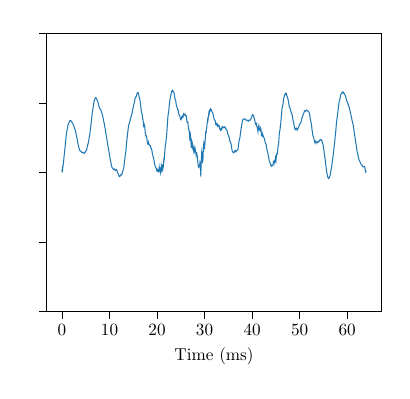
\begin{tikzpicture}[scale=0.62]

\definecolor{darkgray176}{RGB}{176,176,176}
\definecolor{steelblue31119180}{RGB}{31,119,180}

\begin{axis}[
yticklabel={\empty},
tick align=outside,
tick pos=left,
x grid style={darkgray176},
xlabel={Time (ms)},
xmin=-3.2, xmax=67.2,
xtick style={color=black},
y grid style={darkgray176},
% ylabel={Amplitude},
% ymin=-0.15, ymax=0.15,
ymin=-0.1, ymax=0.1,
ytick style={color=black}
]
\addplot [semithick, steelblue31119180]
table {%
0 0
0.0625610948191593 0.00267421979664707
0.125122189638319 0.00195263445792485
0.187683284457478 0.00448575329658223
0.250244379276637 0.00506307051416017
0.312805474095797 0.00741872769886972
0.375366568914956 0.00896099196129705
0.437927663734115 0.0115803680341702
0.500488758553275 0.0133900876509304
0.563049853372434 0.0151754755341063
0.625610948191593 0.0175304286389494
0.688172043010753 0.0195827149455586
0.750733137829912 0.0220035516719752
0.813294232649071 0.0241572310672827
0.875855327468231 0.0260075675241671
0.93841642228739 0.0276190532682753
1.00097751710655 0.029011056083869
1.06353861192571 0.0303319803605681
1.12609970674487 0.0314772311226626
1.18866080156403 0.0323503866813574
1.25122189638319 0.0340090383259345
1.31378299120235 0.0342868589673224
1.37634408602151 0.034962264941104
1.43890518084066 0.0355454103753539
1.50146627565982 0.0360117456070052
1.56402737047898 0.0365307936963797
1.62658846529814 0.0370469956639663
1.6891495601173 0.0372855405697375
1.75171065493646 0.0373638160362883
1.81427174975562 0.0371841114243804
1.87683284457478 0.0371509336557818
1.93939393939394 0.0367688526484099
2.0019550342131 0.0364753106155616
2.06451612903226 0.0361838696464416
2.12707722385142 0.0359691435804378
2.18963831867058 0.0355138606187011
2.25219941348974 0.0352915312351981
2.3147605083089 0.0347998261102134
2.37732160312805 0.0344101194336005
2.43988269794721 0.0336631536920749
2.50244379276637 0.0331262272681571
2.56500488758553 0.0324098647864333
2.62756598240469 0.0318902237095004
2.69012707722385 0.0313611501975318
2.75268817204301 0.030779401080743
2.81524926686217 0.0301372612829257
2.87781036168133 0.0291732079745475
2.94037145650049 0.0278471793837386
3.00293255131965 0.026998937900159
3.06549364613881 0.0261555616457092
3.12805474095797 0.0251639858926059
3.19061583577713 0.0240808387786762
3.25317693059629 0.0226956488526374
3.31573802541544 0.0215881998074457
3.3782991202346 0.0205637725818454
3.44086021505376 0.0194245896512462
3.50342130987292 0.0185915641158907
3.56598240469208 0.0176511272853595
3.62854349951124 0.016837186412203
3.6911045943304 0.0160462343054783
3.75366568914956 0.0156823699676658
3.81622678396872 0.0154439510553638
3.87878787878788 0.0154666042124683
3.94134897360704 0.0152564826052734
4.0039100684262 0.0150434925245487
4.06647116324536 0.01496300729445
4.12903225806452 0.0145273268102638
4.19159335288368 0.0143023412947781
4.25415444770283 0.0141885221670887
4.31671554252199 0.0143579145090496
4.37927663734115 0.0143627272509148
4.44183773216031 0.0143107777445023
4.50439882697947 0.0143003093455631
4.56695992179863 0.0140994674365017
4.62952101661779 0.0139923333422529
4.69208211143695 0.0136977836183788
4.75464320625611 0.013858715826072
4.81720430107527 0.0140708540115626
4.87976539589443 0.0146523808071778
4.94232649071359 0.0149836221114456
5.00488758553275 0.0151687482169821
5.06744868035191 0.0155991362598984
5.13000977517107 0.0159412591371281
5.19257086999022 0.0162529259035227
5.25513196480938 0.017360441337539
5.31769305962854 0.0182014699926999
5.3802541544477 0.0193291187581341
5.44281524926686 0.0200854901912625
5.50537634408602 0.0208316617795537
5.56793743890518 0.0217071624084914
5.63049853372434 0.0229126865049698
5.6930596285435 0.0242266035106175
5.75562072336266 0.0256323526474126
5.81818181818182 0.0267178274013779
5.88074291300098 0.0283921178146279
5.94330400782014 0.0298888944198659
6.0058651026393 0.0314556878562634
6.06842619745846 0.0335125506820042
6.13098729227761 0.0353603800185178
6.19354838709677 0.0371862264169801
6.25610948191593 0.0392754322130921
6.31867057673509 0.0411166230822938
6.38123167155425 0.0428521498174699
6.44379276637341 0.0441375720776246
6.50635386119257 0.0457053787929834
6.56891495601173 0.0472871441710904
6.63147605083089 0.048761960190019
6.69403714565005 0.0498478819788201
6.75659824046921 0.050987220705211
6.81915933528837 0.0516526354504121
6.88172043010753 0.052490993072429
6.94428152492669 0.0530063456738275
7.00684261974585 0.0534649434775289
7.069403714565 0.0537074036634038
7.13196480938416 0.0537072170656885
7.19452590420332 0.0535349667596677
7.25708699902248 0.0530148078673833
7.31964809384164 0.0528068320274003
7.3822091886608 0.0521574912434362
7.44477028347996 0.0515556330096162
7.50733137829912 0.0511457352595857
7.56989247311828 0.0503554332160181
7.63245356793744 0.0496244228928407
7.6950146627566 0.0487227421199297
7.75757575757576 0.0479266882281412
7.82013685239492 0.0471831423031095
7.88269794721408 0.046654381715526
7.94525904203324 0.0460351152001413
8.00782013685239 0.0457550140146898
8.07038123167155 0.0454348212550462
8.13294232649071 0.0452133226112798
8.19550342130987 0.0445972337685198
8.25806451612903 0.0439055550603136
8.32062561094819 0.0433501996252893
8.38318670576735 0.0427576806942476
8.44574780058651 0.0420135908768324
8.50830889540567 0.0413939108542246
8.57086999022483 0.040383708649629
8.63343108504399 0.0394220507029127
8.69599217986315 0.0382373149225439
8.75855327468231 0.0370243414417128
8.82111436950147 0.0361064742824549
8.88367546432062 0.0353182733026156
8.94623655913978 0.034049863776853
9.00879765395894 0.0328304045656122
9.0713587487781 0.0317752120300822
9.13391984359726 0.0303793267955965
9.19648093841642 0.0287503501471361
9.25904203323558 0.0277123870792364
9.32160312805474 0.0264058492072691
9.3841642228739 0.0252075347437624
9.44672531769306 0.0238300412674803
9.50928641251222 0.0225178186025176
9.57184750733138 0.0210519984932589
9.63440860215054 0.0198594470538439
9.6969696969697 0.0187120908363299
9.75953079178886 0.0173988586176962
9.82209188660802 0.0162397695983872
9.88465298142718 0.0150185930283188
9.94721407624633 0.0135728019423499
10.0097751710655 0.0123385272515921
10.0723362658847 0.0110240861762566
10.1348973607038 0.00961095098504398
10.197458455523 0.00825266510554073
10.2600195503421 0.0075971999443259
10.3225806451613 0.00651535481935547
10.3851417399804 0.00549221840684365
10.4477028347996 0.00441473745945787
10.5102639296188 0.00380801213386297
10.5728250244379 0.00333096788884782
10.6353861192571 0.0030224520516448
10.6979472140762 0.00274330640315485
10.7605083088954 0.00251342399357176
10.8230694037146 0.00208306508657695
10.8856304985337 0.00217947526630069
10.9481915933529 0.00227255503649761
11.010752688172 0.00244182444387867
11.0733137829912 0.00224105331533291
11.1358748778104 0.00175680994681599
11.1984359726295 0.00137892175367501
11.2609970674487 0.0013601645838218
11.3235581622678 0.001649708713779
11.386119257087 0.00193779625522951
11.4486803519062 0.00198972274349931
11.5112414467253 0.00166785174057631
11.5738025415445 0.00142994691833548
11.6363636363636 0.00061140903695063
11.6989247311828 -0.000307942650491191
11.761485826002 -0.000503915605132532
11.8240469208211 -0.00113124737401337
11.8866080156403 -0.00155196709236092
11.9491691104594 -0.00214502619049591
12.0117302052786 -0.00279614021264213
12.0742913000978 -0.00304161296212429
12.1368523949169 -0.00297893156076282
12.1994134897361 -0.00285662688817447
12.2619745845552 -0.00236801814582865
12.3245356793744 -0.0021942504504122
12.3870967741935 -0.00160614665477507
12.4496578690127 -0.00156108215123502
12.5122189638319 -0.0018311939707512
12.574780058651 -0.00173706366869012
12.6373411534702 -0.000912511972519309
12.6999022482893 -0.000196902665836721
12.7624633431085 0.000736978850013351
12.8250244379277 0.00106108622335968
12.8875855327468 0.00214182240806542
12.950146627566 0.00270913908383713
13.0127077223851 0.00340024156829129
13.0752688172043 0.00556807706673299
13.1378299120235 0.00725564627725183
13.2003910068426 0.00904701511400187
13.2629521016618 0.0112418273021399
13.3255131964809 0.0124709883655621
13.3880742913001 0.0139866596431938
13.4506353861193 0.0154722398884398
13.5131964809384 0.0179199806613919
13.5757575757576 0.0204215760935437
13.6383186705767 0.0226809065843607
13.7008797653959 0.0248251628578583
13.7634408602151 0.0266148869789416
13.8260019550342 0.0284216282261082
13.8885630498534 0.0303372205931508
13.9511241446725 0.0320307074273087
14.0136852394917 0.0336226689249627
14.0762463343109 0.0342720239436871
14.13880742913 0.0349491323751351
14.2013685239492 0.0356921560931241
14.2639296187683 0.0364141654485394
14.3264907135875 0.0373742953598325
14.3890518084066 0.0380467732554394
14.4516129032258 0.0389382684182736
14.514173998045 0.039927060713123
14.5767350928641 0.0404909389459493
14.6392961876833 0.0411950073032872
14.7018572825024 0.0419001485442311
14.7644183773216 0.0429625525753781
14.8269794721408 0.0438603695558488
14.8895405669599 0.0452642597727849
14.9521016617791 0.0463684541105001
15.0146627565982 0.0474161693220002
15.0772238514174 0.0484258940230367
15.1397849462366 0.048982958699907
15.2023460410557 0.0497803344033506
15.2649071358749 0.051131768807594
15.327468230694 0.0521033428106839
15.3900293255132 0.0531876813511083
15.4525904203324 0.0538189128325307
15.5151515151515 0.0541310210458257
15.5777126099707 0.0543522023735158
15.6402737047898 0.0549303894463785
15.702834799609 0.0555825384328267
15.7653958944282 0.0564133933201826
15.8279569892473 0.056831538196533
15.8905180840665 0.0572587951329534
15.9530791788856 0.057280189141937
16.0156402737048 0.0573616571822736
16.0782013685239 0.056989228402065
16.1407624633431 0.0559466459741952
16.2033235581623 0.0549218033787267
16.2658846529814 0.0539930620970876
16.3284457478006 0.0531750289925382
16.3910068426197 0.0521099569871366
16.4535679374389 0.0510703175386026
16.5161290322581 0.0493302415575712
16.5786901270772 0.0474945895286424
16.6412512218964 0.0456468005039213
16.7038123167155 0.0437111058040274
16.7663734115347 0.0426618811835554
16.8289345063539 0.0419866980607908
16.891495601173 0.0413465699197348
16.9540566959922 0.0398208843953798
17.0166177908113 0.0385363369120443
17.0791788856305 0.0372270050723532
17.1417399804497 0.0345423184062117
17.2043010752688 0.032461166021324
17.266862170088 0.0347551361239813
17.3294232649071 0.0341661413175619
17.3919843597263 0.0338865765739134
17.4545454545455 0.0314861332828348
17.5171065493646 0.0286533663273295
17.5796676441838 0.0271085365361307
17.6422287390029 0.0262852582228411
17.7047898338221 0.0263691197621945
17.7673509286412 0.0262591917002219
17.8299120234604 0.0251460206091317
17.8924731182796 0.023419109804015
17.9550342130987 0.0213664465766848
18.0175953079179 0.0208063320833043
18.080156402737 0.0203971048855275
18.1427174975562 0.0208537711262091
18.2052785923754 0.0216071604644536
18.2678396871945 0.020109887729205
18.3304007820137 0.0199684586124686
18.3929618768328 0.0197349161051673
18.455522971652 0.0194785226671752
18.5180840664712 0.0194128193889807
18.5806451612903 0.0193844509701575
18.6432062561095 0.0188214922176341
18.7057673509286 0.0173547650001878
18.7683284457478 0.0172885383187064
18.830889540567 0.0166502374325417
18.8934506353861 0.0162434242228783
18.9560117302053 0.0150629650757722
19.0185728250244 0.013391328265459
19.0811339198436 0.0127082065490683
19.1436950146628 0.0115744774434661
19.2062561094819 0.0109363535085906
19.2688172043011 0.0104743799254779
19.3313782991202 0.00898958691272917
19.3939393939394 0.00790707682344046
19.4565004887586 0.0066469337168502
19.5190615835777 0.00564898771733657
19.5816226783969 0.0047800187185363
19.644183773216 0.00409872611968224
19.7067448680352 0.00366864474681465
19.7693059628544 0.00332232838895314
19.8318670576735 0.00288059430803197
19.8944281524927 0.00273982084238809
19.9569892473118 0.000845879196159301
20.019550342131 0.000760033273321092
20.0821114369501 0.00095205489120001
20.1446725317693 0.0019063416846599
20.2072336265885 0.00162790942926211
20.2697947214076 0.000875847490608168
20.3323558162268 0.000575767573286014
20.3949169110459 0.00160671152786251
20.4574780058651 0.00388647337332149
20.5200391006843 0.00233205468489453
20.5826001955034 0.00152916488540837
20.6451612903226 0.00328123563479993
20.7077223851417 0.00326864568303582
20.7702834799609 -0.00020999720325568
20.8328445747801 0.000763068778598764
20.8954056695992 0.00438050786442945
20.9579667644184 0.0029384327555332
21.0205278592375 0.000206796255760179
21.0830889540567 0.00278985447351359
21.1456500488759 0.00508365880075263
21.208211143695 0.00488976083280753
21.2707722385142 0.00338998097718811
21.3333333333333 0.00464094616472721
21.3958944281525 0.00786668587683582
21.4584555229717 0.0097706981789856
21.5210166177908 0.00937353533384038
21.58357771261 0.0119085969113884
21.6461388074291 0.0154543465107155
21.7086999022483 0.0183054468160238
21.7712609970674 0.0201115640770655
21.8338220918866 0.0206162288205977
21.8963831867058 0.0229037094675551
21.9589442815249 0.0247902948616886
22.0215053763441 0.0266693644826451
22.0840664711632 0.030081022257679
22.1466275659824 0.0328973525659867
22.2091886608016 0.0361175192438088
22.2717497556207 0.0395221697477913
22.3343108504399 0.041304173204731
22.396871945259 0.0427716355006104
22.4594330400782 0.0439727842436333
22.5219941348974 0.04629844911615
22.5845552297165 0.0490542658088494
22.6471163245357 0.0508796651724759
22.7096774193548 0.0520982259223538
22.772238514174 0.0532420461729737
22.8347996089932 0.0545685695609914
22.8973607038123 0.0551733477560044
22.9599217986315 0.0559879976305619
23.0224828934506 0.0578949249723702
23.0850439882698 0.0583804640755101
23.147605083089 0.0584930904439031
23.2101661779081 0.0588970233377648
23.2727272727273 0.0583844416859475
23.3352883675464 0.0586766382225972
23.3978494623656 0.0583387540593263
23.4604105571848 0.0581928974350701
23.5229716520039 0.0575271020438577
23.5855327468231 0.0569285704942742
23.6480938416422 0.0559307399787599
23.7106549364614 0.0543003477199861
23.7732160312805 0.0534002241184198
23.8357771260997 0.0520780251260377
23.8983382209189 0.0516900767864457
23.960899315738 0.0508313895888692
24.0234604105572 0.049175866521742
24.0860215053763 0.0479400197584783
24.1485826001955 0.0473373903895665
24.2111436950147 0.046511578878874
24.2737047898338 0.0462514713264543
24.336265884653 0.0451448697848054
24.3988269794721 0.0451817311991083
24.4613880742913 0.0443530065114023
24.5239491691105 0.0426578202784673
24.5865102639296 0.0416546216196329
24.6490713587488 0.0413088361156389
24.7116324535679 0.041108225174576
24.7741935483871 0.0408650341654016
24.8367546432063 0.0398515648812143
24.8993157380254 0.038847956440447
24.9618768328446 0.0380346358281252
25.0244379276637 0.0378304746854078
25.0869990224829 0.0382387661689188
25.1495601173021 0.0390100164114992
25.2121212121212 0.0399538556283171
25.2746823069404 0.040413034577305
25.3372434017595 0.0400065938966715
25.3998044965787 0.0394734188400843
25.4623655913978 0.0394740778832666
25.524926686217 0.0411028750513918
25.5874877810362 0.0420756560485384
25.6500488758553 0.0417780720757162
25.7126099706745 0.0412677814774324
25.7751710654936 0.041175230032057
25.8377321603128 0.0413646532599527
25.900293255132 0.0417800190697405
25.9628543499511 0.0412614583269941
26.0254154447703 0.0406542915544989
26.0879765395894 0.0408050164667742
26.1505376344086 0.0405792076621325
26.2130987292278 0.0390043036023543
26.2756598240469 0.0368666124866068
26.3382209188661 0.0360929401389315
26.4007820136852 0.0362097313818781
26.4633431085044 0.036331480986212
26.5259042033236 0.0345905183860896
26.5884652981427 0.031986461903168
26.6510263929619 0.031094742556515
26.713587487781 0.0309626471546214
26.7761485826002 0.0293936625811274
26.8387096774194 0.0263035376706431
26.9012707722385 0.0239715223744118
26.9638318670577 0.0245473122229674
27.0263929618768 0.026747274624943
27.088954056696 0.0248879576893933
27.1515151515152 0.0209304007955573
27.2140762463343 0.0176937769814408
27.2766373411535 0.0196157470454743
27.3391984359726 0.0221516430880492
27.4017595307918 0.0213706412317117
27.4643206256109 0.0188635372914527
27.5268817204301 0.0167689943505872
27.5894428152493 0.0163053760518077
27.6520039100684 0.0177176835621732
27.7145650048876 0.0165713070960076
27.7771260997067 0.0141103166617082
27.8396871945259 0.0146560471428454
27.9022482893451 0.0159809314031318
27.9648093841642 0.0179326702619403
28.0273704789834 0.0170464531690581
28.0899315738025 0.0151981798565982
28.1524926686217 0.0144559601349128
28.2150537634409 0.0127864169377473
28.27761485826 0.0140569939160627
28.3401759530792 0.0141271333486017
28.4027370478983 0.0123410444444488
28.4652981427175 0.0116867676508392
28.5278592375367 0.00907893372355493
28.5904203323558 0.00709933834013876
28.652981427175 0.00512608153816542
28.7155425219941 0.00378594341035113
28.7781036168133 0.00356751068050036
28.8406647116325 0.00437589089148555
28.9032258064516 0.00465376368693767
28.9657869012708 0.00537902522078357
29.0283479960899 0.00695361941506611
29.0909090909091 0.00594923797656189
29.1534701857282 0.0013902217881683
29.2160312805474 -0.00304396178496898
29.2785923753666 0.00566547975228154
29.3411534701857 0.0108653606896089
29.4037145650049 0.014694018147427
29.466275659824 0.0133876833037809
29.5288367546432 0.0101675867400736
29.5913978494624 0.00803752129356707
29.6539589442815 0.00901241266766776
29.7165200391007 0.0144135524133696
29.7790811339198 0.0189351138667015
29.841642228739 0.0207817511103195
29.9042033235582 0.0193139174816545
29.9667644183773 0.0165541066113543
30.0293255131965 0.0189539923051323
30.0918866080156 0.0218169781491379
30.1544477028348 0.0246398184022421
30.217008797654 0.0282433863696465
30.2795698924731 0.0278777189913296
30.3421309872923 0.0289339464911617
30.4046920821114 0.0309737586632065
30.4672531769306 0.0327821483513302
30.5298142717498 0.0346808726039013
30.5923753665689 0.0366036100777363
30.6549364613881 0.0380971568562855
30.7174975562072 0.0375351592286591
30.7800586510264 0.0395417567124028
30.8426197458456 0.0406106800015721
30.9051808406647 0.0431468461276936
30.9677419354839 0.0440592289932313
31.030303030303 0.0431223926557736
31.0928641251222 0.044251091953072
31.1554252199413 0.044091906240128
31.2179863147605 0.0447321454734921
31.2805474095797 0.0457030936278119
31.3431085043988 0.0453781697494893
31.405669599218 0.0451644942153496
31.4682306940371 0.0443997886414227
31.5307917888563 0.0437652633369756
31.5933528836755 0.0434029524452176
31.6559139784946 0.043035791225491
31.7184750733138 0.0426897188741441
31.7810361681329 0.0420002157354722
31.8435972629521 0.0409411973268056
31.9061583577713 0.039571873412148
31.9687194525904 0.0386384047371202
32.0312805474096 0.0383785877573438
32.0938416422287 0.0375490882092557
32.1564027370479 0.0375753101944661
32.2189638318671 0.0374420748537412
32.2815249266862 0.0360706945788388
32.3440860215054 0.0350615131037851
32.4066471163245 0.0339929430507932
32.4692082111437 0.0340246002345491
32.5317693059629 0.0349592938636842
32.594330400782 0.0352224107842641
32.6568914956012 0.034789714257607
32.7194525904203 0.0336865213565812
32.7820136852395 0.0331596681176305
32.8445747800587 0.0334299338702932
32.9071358748778 0.0338081808875471
32.969696969697 0.033365224911408
33.0322580645161 0.0329333330474554
33.0948191593353 0.0332109972266508
33.1573802541544 0.0320883396838155
33.2199413489736 0.0309007317046266
33.2825024437928 0.0308718603716131
33.3450635386119 0.030459921162499
33.4076246334311 0.0313069512603307
33.4701857282502 0.0315470496121565
33.5327468230694 0.0310009366223627
33.5953079178886 0.0306450518563696
33.6578690127077 0.0318058445295892
33.7204301075269 0.0329603675392366
33.782991202346 0.0327633887562147
33.8455522971652 0.032416258422423
33.9081133919844 0.0322558210119387
33.9706744868035 0.0320788991918837
34.0332355816227 0.0323125378903318
34.0957966764418 0.0326428515973154
34.158357771261 0.0326298984297472
34.2209188660802 0.032318359519467
34.2834799608993 0.0326219256421076
34.3460410557185 0.0323100589062811
34.4086021505376 0.0318218369277254
34.4711632453568 0.0310809285082251
34.533724340176 0.0310058263226076
34.5962854349951 0.0309875087370096
34.6588465298143 0.0306313110466315
34.7214076246334 0.0300611066044775
34.7839687194526 0.0293552047379118
34.8465298142717 0.0284407946480509
34.9090909090909 0.0275458454747092
34.9716520039101 0.0268777255023505
35.0342130987292 0.0267992109508196
35.0967741935484 0.0259139400816733
35.1593352883675 0.0252057173592516
35.2218963831867 0.0244404716182314
35.2844574780059 0.0227533189738251
35.347018572825 0.0225678494751803
35.4095796676442 0.0221244483268506
35.4721407624633 0.0217717170190951
35.5347018572825 0.0210364933925902
35.5972629521017 0.0201191887521674
35.6598240469208 0.0188929513752286
35.72238514174 0.0170571037685591
35.7849462365591 0.0159716786396119
35.8475073313783 0.0150278387563931
35.9100684261975 0.01489631146127
35.9726295210166 0.0146592597305076
36.0351906158358 0.0141087751125485
36.0977517106549 0.014124936951308
36.1603128054741 0.014254863567847
36.2228739002933 0.0143559359483792
36.2854349951124 0.0151110854862897
36.3479960899316 0.0150740762566192
36.4105571847507 0.0157257782082316
36.4731182795699 0.0156458070681941
36.5356793743891 0.0150090577654388
36.5982404692082 0.0147384244052808
36.6608015640274 0.015120394850188
36.7233626588465 0.0154524166027734
36.7859237536657 0.0158782299892032
36.8484848484849 0.0158998847685077
36.911045943304 0.0161424008337371
36.9736070381232 0.0162015636984117
37.0361681329423 0.0167102424422405
37.0987292277615 0.0182204747960365
37.1612903225806 0.0200580241939714
37.2238514173998 0.0217561341133897
37.286412512219 0.0231641612652023
37.3489736070381 0.0238318093219373
37.4115347018573 0.0247525442883241
37.4740957966764 0.025644510700381
37.5366568914956 0.0275202778514879
37.5992179863148 0.0292770331534298
37.6617790811339 0.0308391401746318
37.7243401759531 0.0322980790063083
37.7869012707722 0.0334602463116482
37.8494623655914 0.0347619480904072
37.9120234604106 0.0359631676139457
37.9745845552297 0.0368996791847465
38.0371456500489 0.0378674757434738
38.099706744868 0.0381146148939636
38.1622678396872 0.0383059976245563
38.2248289345064 0.0384774612279232
38.2873900293255 0.0383171840049217
38.3499511241447 0.0384484256489361
38.4125122189638 0.0384597241212109
38.475073313783 0.0384790841216915
38.5376344086022 0.0383175552011498
38.6001955034213 0.0377998699016235
38.6627565982405 0.0377321959448612
38.7253176930596 0.0376487938124588
38.7878787878788 0.0376734474504536
38.8504398826979 0.0375150216967304
38.9130009775171 0.0375846544897888
38.9755620723363 0.0374904452902306
39.0381231671554 0.0374442960608128
39.1006842619746 0.0372936971420067
39.1632453567937 0.0369457174420269
39.2258064516129 0.0368236430710362
39.2883675464321 0.0373380606245697
39.3509286412512 0.0374558800476387
39.4134897360704 0.0376636466049641
39.4760508308895 0.0376178475528344
39.5386119257087 0.0375941767250775
39.6011730205279 0.0375067810814751
39.663734115347 0.0377316429959801
39.7262952101662 0.0381126951568287
39.7888563049853 0.0388838746188935
39.8514173998045 0.0394202564840268
39.9139784946237 0.0397456081043328
39.9765395894428 0.040315290339444
40.039100684262 0.0412298003457421
40.1016617790811 0.0414068146316537
40.1642228739003 0.0410492199574136
40.2267839687195 0.0411880649189271
40.2893450635386 0.0409462820694856
40.3519061583578 0.0401449904195374
40.4144672531769 0.0390465733406743
40.4770283479961 0.0386799932662343
40.5395894428152 0.0376865399668206
40.6021505376344 0.0366314517394189
40.6647116324536 0.0358175872347135
40.7272727272727 0.0348084318366918
40.7898338220919 0.0344157486531304
40.852394916911 0.0347675312081041
40.9149560117302 0.0350688882335977
40.9775171065494 0.0333061736634225
41.0400782013685 0.032600074356471
41.1026392961877 0.0321379145088434
41.1652003910068 0.0307046050080194
41.227761485826 0.0294969624176053
41.2903225806452 0.0325823667188806
41.3528836754643 0.0329074016895112
41.4154447702835 0.0337845209570836
41.4780058651026 0.0325840122975912
41.5405669599218 0.0306703675909738
41.603128054741 0.0305694714953298
41.6656891495601 0.030171353113223
41.7282502443793 0.031143564140954
41.7908113391984 0.0318894302554407
41.8533724340176 0.0306748176468782
41.9159335288368 0.0292985609669752
41.9784946236559 0.0267994198347292
42.0410557184751 0.0260753441394424
42.1036168132942 0.026039359364604
42.1661779081134 0.0267842792553549
42.2287390029325 0.0277295210439701
42.2913000977517 0.0265493077660236
42.3538611925709 0.0261299217016029
42.41642228739 0.0255084721661034
42.4789833822092 0.0248335181486921
42.5415444770283 0.0245418480742187
42.6041055718475 0.0241732470297918
42.6666666666667 0.0232807192951441
42.7292277614858 0.0216111164933338
42.791788856305 0.0214149535488873
42.8543499511241 0.0207516336130781
42.9169110459433 0.0204178342306194
42.9794721407625 0.0192357806592655
43.0420332355816 0.0175879018878307
43.1045943304008 0.0168795692693453
43.1671554252199 0.0155753857808466
43.2297165200391 0.0148914705776224
43.2922776148583 0.0144289083986426
43.3548387096774 0.0130980704580584
43.4173998044966 0.0120939013611012
43.4799608993157 0.0108472363548108
43.5425219941349 0.00960976536497692
43.6050830889541 0.00849363266809944
43.6676441837732 0.00765429090304284
43.7302052785924 0.00705099843245797
43.7927663734115 0.00663502100866037
43.8553274682307 0.00606322959283929
43.9178885630498 0.00568777587690836
43.980449657869 0.00445893265940576
44.0430107526882 0.00439443637526804
44.1055718475073 0.00446561516380031
44.1681329423265 0.00513564554368121
44.2306940371457 0.00521406070861823
44.2932551319648 0.00499794883462341
44.355816226784 0.00488837840051945
44.4183773216031 0.00564268229753216
44.4809384164223 0.00737928005366906
44.5434995112414 0.00707713632552155
44.6060606060606 0.0070919179442254
44.6686217008798 0.00851020454551992
44.7311827956989 0.00866406987751684
44.7937438905181 0.00704828820729361
44.8563049853372 0.00816068935953627
44.9188660801564 0.0108787558229962
44.9814271749756 0.010371167922824
45.0439882697947 0.00914865583618366
45.1065493646139 0.0114646889706336
45.169110459433 0.0132357996787406
45.2316715542522 0.0134156004817954
45.2942326490714 0.0132334446288711
45.3567937438905 0.0144499974472781
45.4193548387097 0.0173056817222987
45.4819159335288 0.019130442198639
45.544477028348 0.0196244097710792
45.6070381231672 0.021854941905244
45.6695992179863 0.025132772351596
45.7321603128055 0.0278786127168762
45.7947214076246 0.0295117591614248
45.8572825024438 0.0303778906852619
45.919843597263 0.0322564648426086
45.9824046920821 0.0339553831500217
46.0449657869013 0.0358612972128688
46.1075268817204 0.0385077691847278
46.1700879765396 0.0408807266175834
46.2326490713588 0.0432648152178508
46.2952101661779 0.0456662636709091
46.3577712609971 0.046847217615224
46.4203323558162 0.0477867429458763
46.4828934506354 0.0485950412004749
46.5454545454545 0.0505165232514793
46.6080156402737 0.0525513137322018
46.6705767350929 0.0537294811593735
46.733137829912 0.0543446789913513
46.7956989247312 0.0549502618490688
46.8582600195503 0.0558704715495235
46.9208211143695 0.0559133530329487
46.9833822091887 0.0559761648194706
47.0459433040078 0.0569916450940182
47.108504398827 0.0570250419883434
47.1710654936461 0.0568927230690319
47.2336265884653 0.056640900562236
47.2961876832845 0.0551848630653011
47.3587487781036 0.0547586485437634
47.4213098729228 0.0541026841936486
47.4838709677419 0.0536307193819554
47.5464320625611 0.0527246055135891
47.6089931573803 0.0517289356664479
47.6715542521994 0.0508142424545243
47.7341153470186 0.0493116723564713
47.7966764418377 0.0481130375179989
47.8592375366569 0.0468085671821473
47.9217986314761 0.0465829856202137
47.9843597262952 0.0462157163670685
48.0469208211144 0.0452095076736729
48.1094819159335 0.0442796264532025
48.1720430107527 0.0438324161955426
48.2346041055718 0.0430557673409188
48.297165200391 0.0426278280099728
48.3597262952102 0.0418391911711686
48.4222873900293 0.041594998058904
48.4848484848485 0.0406052067198537
48.5474095796676 0.0389845076664365
48.6099706744868 0.0375579707433751
48.672531769306 0.0365544479842847
48.7350928641251 0.0357116901280244
48.7976539589443 0.0348651324756596
48.8602150537634 0.0336367660953153
48.9227761485826 0.0324083252091649
48.9853372434018 0.0313928293670552
49.0478983382209 0.0309147811563046
49.1104594330401 0.030692954686992
49.1730205278592 0.0309709876699269
49.2355816226784 0.031597696648927
49.2981427174976 0.0318774469906896
49.3607038123167 0.0314093900085195
49.4232649071359 0.0308339031047223
49.485826001955 0.0304353637648118
49.5483870967742 0.031060064812341
49.6109481915934 0.0315283893490117
49.6735092864125 0.031664160946029
49.7360703812317 0.0318912170565198
49.7986314760508 0.0325307298582757
49.86119257087 0.0333566375601152
49.9237536656891 0.0340274055474752
49.9863147605083 0.0343475082337507
50.0488758553275 0.0348904801374219
50.1114369501466 0.0352367120098508
50.1739980449658 0.0354705928521684
50.2365591397849 0.0357889670037454
50.2991202346041 0.0362658038287481
50.3616813294233 0.0370228979681944
50.4242424242424 0.0380117535929788
50.4868035190616 0.0389377374933962
50.5493646138807 0.0395894841484922
50.6119257086999 0.0399620687244924
50.6744868035191 0.0408489817802595
50.7370478983382 0.0415870843897642
50.7996089931574 0.0421664896325544
50.8621700879765 0.0424486465118498
50.9247311827957 0.04317258929293
50.9872922776149 0.0436714500341772
51.049853372434 0.0439890157977594
51.1124144672532 0.044358433877006
51.1749755620723 0.0441271898738188
51.2375366568915 0.0438700103995737
51.3000977517107 0.0442643841985296
51.3626588465298 0.0446783232221331
51.425219941349 0.0449076517597059
51.4877810361681 0.0448242272755617
51.5503421309873 0.0448317967322477
51.6129032258064 0.0444544803711676
51.6754643206256 0.0442608096459307
51.7380254154448 0.0440060031816057
51.8005865102639 0.0440069565227217
51.8631476050831 0.0439781410690626
51.9257086999022 0.0437708097043013
51.9882697947214 0.0431585281082262
52.0508308895406 0.0425149987771277
52.1133919843597 0.0415439978023428
52.1759530791789 0.0401725728239569
52.238514173998 0.0387360111447024
52.3010752688172 0.0377038967825713
52.3636363636364 0.0366723598404364
52.4261974584555 0.0354431589950652
52.4887585532747 0.0341393890137896
52.5513196480938 0.0325012071730017
52.613880742913 0.0306788693315997
52.6764418377322 0.0291148989988475
52.7390029325513 0.0275694079686208
52.8015640273705 0.0265256427610812
52.8641251221896 0.0256399043680024
52.9266862170088 0.0253011354482856
52.989247311828 0.0243811560494284
53.0518084066471 0.0233437759894605
53.1143695014663 0.0225893578046927
53.1769305962854 0.0217172744632029
53.2394916911046 0.0211648024028697
53.3020527859238 0.0224554698717647
53.3646138807429 0.0222937956649013
53.4271749755621 0.0224200454199157
53.4897360703812 0.0216772929817176
53.5522971652004 0.0212178265189757
53.6148582600196 0.0211791725736385
53.6774193548387 0.0211344315039535
53.7399804496579 0.0214040229790721
53.802541544477 0.0220809991627145
53.8651026392962 0.0223197899376455
53.9276637341153 0.0223311759542423
53.9902248289345 0.0219567615943046
54.0527859237537 0.0220094107888923
54.1153470185728 0.0223439676015258
54.177908113392 0.0227976033185497
54.2404692082111 0.0232850162427097
54.3030303030303 0.0231732385741039
54.3655913978495 0.0234766053937135
54.4281524926686 0.0236280772266937
54.4907135874878 0.0235211834136692
54.5532746823069 0.0233881529639106
54.6158357771261 0.0231276766077514
54.6783968719453 0.0227126081547867
54.7409579667644 0.0217724376825119
54.8035190615836 0.0213462827656189
54.8660801564027 0.0205169620314651
54.9286412512219 0.020012508963079
54.9912023460411 0.0188231631359659
55.0537634408602 0.0171258385863996
55.1163245356794 0.0157880976828924
55.1788856304985 0.0139106013306862
55.2414467253177 0.0122885611727615
55.3040078201369 0.0112943628152882
55.366568914956 0.0093972099688221
55.4291300097752 0.00770373364413414
55.4916911045943 0.00584246838175831
55.5542521994135 0.00412534391425572
55.6168132942326 0.00245839351913796
55.6793743890518 0.000780038147771465
55.741935483871 -0.000622202431963335
55.8044965786901 -0.00163171173256339
55.8670576735093 -0.00270341847998656
55.9296187683284 -0.00340635501547468
55.9921798631476 -0.00384208765372503
56.0547409579668 -0.00413895264551961
56.1173020527859 -0.00444098088966786
56.1798631476051 -0.00418070636558568
56.2424242424242 -0.00360199775208126
56.3049853372434 -0.00304885953118549
56.3675464320626 -0.00252012568703495
56.4301075268817 -0.0017775341027206
56.4926686217009 -0.000825290630989413
56.55522971652 0.000563787831720022
56.6177908113392 0.00183773806040063
56.6803519061584 0.00313017317954221
56.7429130009775 0.00412363140049044
56.8054740957967 0.00566291729332415
56.8680351906158 0.00711228026628844
56.930596285435 0.0089067299181153
56.9931573802542 0.0104306080102746
57.0557184750733 0.0119805407827813
57.1182795698925 0.0143055500042054
57.1808406647116 0.0158458994674193
57.2434017595308 0.0175163397931458
57.3059628543499 0.0196888505309121
57.3685239491691 0.0215753390674979
57.4310850439883 0.023990589721112
57.4936461388074 0.0260414846317946
57.5562072336266 0.0279752023987844
57.6187683284457 0.0300400056807963
57.6813294232649 0.03277259705113
57.7438905180841 0.0352639255832193
57.8064516129032 0.0372064629749906
57.8690127077224 0.0387646770678308
57.9315738025415 0.0404650743154924
57.9941348973607 0.0420708640907342
58.0566959921799 0.0439263153711984
58.119257086999 0.0457073502526605
58.1818181818182 0.0474987526170232
58.2443792766373 0.0490374536392801
58.3069403714565 0.0505239223662622
58.3695014662757 0.0515297504136464
58.4320625610948 0.0522976404443777
58.494623655914 0.0528898979386976
58.5571847507331 0.0540614753273313
58.6197458455523 0.0552708644124944
58.6823069403715 0.0560077898302648
58.7448680351906 0.0564124975845087
58.8074291300098 0.0568147131195428
58.8699902248289 0.0571315971550005
58.9325513196481 0.0569640071871431
58.9951124144673 0.0570515101977632
59.0576735092864 0.0578324908986032
59.1202346041056 0.0576970315595701
59.1827956989247 0.057722884741041
59.2453567937439 0.0576931007119043
59.307917888563 0.0567069899596689
59.3704789833822 0.0566763006849897
59.4330400782014 0.05626079637306
59.4956011730205 0.0559517869348925
59.5581622678397 0.0556505410017069
59.6207233626588 0.055134919513006
59.683284457478 0.0544264769984568
59.7458455522972 0.053288635172365
59.8084066471163 0.0526271909202211
59.8709677419355 0.0517917160064943
59.9335288367546 0.0514830865479372
59.9960899315738 0.051134827451185
60.058651026393 0.0505215214002779
60.1212121212121 0.0497802963311022
60.1837732160313 0.0491487996876677
60.2463343108504 0.0484007759636973
60.3088954056696 0.0478875684631098
60.3714565004888 0.0473363406497362
60.4340175953079 0.0468872565710562
60.4965786901271 0.0460121147662314
60.5591397849462 0.0450108979618357
60.6217008797654 0.0438298725706042
60.6842619745846 0.0428822552430228
60.7468230694037 0.0419466333502024
60.8093841642229 0.0411196371971949
60.871945259042 0.0403209532504557
60.9345063538612 0.039276586408533
60.9970674486804 0.0380582447843817
61.0596285434995 0.0371007740639609
61.1221896383187 0.0360698294429835
61.1847507331378 0.0353156627153109
61.247311827957 0.0343963464181269
61.3098729227762 0.0335445323811511
61.3724340175953 0.031944404380762
61.4349951124145 0.0303682355849274
61.4975562072336 0.0286385904167317
61.5601173020528 0.0272719170461215
61.6226783968719 0.0258196607188395
61.6852394916911 0.0243035696796483
61.7478005865103 0.0227989208696088
61.8103616813294 0.021500640103588
61.8729227761486 0.0203646199444522
61.9354838709677 0.0187503377035741
61.9980449657869 0.0170625145069141
62.0606060606061 0.0159145622429523
62.1231671554252 0.0145981244120168
62.1857282502444 0.0137994386026324
62.2482893450635 0.012727528826888
62.3108504398827 0.0117746551146955
62.3734115347019 0.0107542865928754
62.435972629521 0.00994687242832177
62.4985337243402 0.00900293568755525
62.5610948191593 0.00859378858351987
62.6236559139785 0.00813819083475298
62.6862170087977 0.00771863340697855
62.7487781036168 0.00717838961205
62.811339198436 0.00671188235064406
62.8739002932551 0.00621034618456168
62.9364613880743 0.00593350649076647
62.9990224828935 0.0054801793064365
63.0615835777126 0.00537889578060146
63.1241446725318 0.00507545192613979
63.1867057673509 0.0048174845529966
63.2492668621701 0.00437471670401761
63.3118279569892 0.00417060399007413
63.3743890518084 0.00395582949529645
63.4369501466276 0.00400284605095289
63.4995112414467 0.00400681501456544
63.5620723362659 0.00419773767180632
63.624633431085 0.00398296317702864
63.6871945259042 0.00392700898354529
63.7497556207234 0.0032044941848936
63.8123167155425 0.00166316802922057
63.8748778103617 0.000470869909545896
63.9374389051808 0.000761237328659056
64 0
};
\end{axis}

\end{tikzpicture}

	\end{subfigure}\hfill
	\begin{subfigure}{0.3\textwidth}
		\centering
		% This file was created with tikzplotlib v0.10.1.
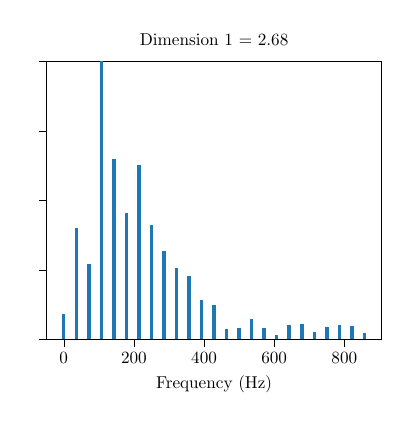
\begin{tikzpicture}[scale=0.62]

\definecolor{darkgray176}{RGB}{176,176,176}
\definecolor{steelblue31119180}{RGB}{31,119,180}

\begin{axis}[
yticklabel={\empty},
tick align=outside,
tick pos=left,
x grid style={darkgray176},
xlabel={Frequency (Hz)},
xmin=-48.3571428571429, xmax=905.5,
xtick style={color=black},
y grid style={darkgray176},
%ylabel={Magnitude},
ymin=0, ymax=4,
title={Dimension 1 = 2.68},
ytick style={color=black}
]
\draw[draw=none,fill=steelblue31119180] (axis cs:-5,0) rectangle (axis cs:5,0.363293109461665);
\draw[draw=none,fill=steelblue31119180] (axis cs:30.7142857142857,0) rectangle (axis cs:40.7142857142857,1.59671692845371);
\draw[draw=none,fill=steelblue31119180] (axis cs:66.4285714285714,0) rectangle (axis cs:76.4285714285714,1.08375129075336);
\draw[draw=none,fill=steelblue31119180] (axis cs:102.142857142857,0) rectangle (axis cs:112.142857142857,5.72028640718505);
\draw[draw=none,fill=steelblue31119180] (axis cs:137.857142857143,0) rectangle (axis cs:147.857142857143,2.60109171070077);
\draw[draw=none,fill=steelblue31119180] (axis cs:173.571428571429,0) rectangle (axis cs:183.571428571429,1.82230187959835);
\draw[draw=none,fill=steelblue31119180] (axis cs:209.285714285714,0) rectangle (axis cs:219.285714285714,2.50466396839656);
\draw[draw=none,fill=steelblue31119180] (axis cs:245,0) rectangle (axis cs:255,1.64154431128106);
\draw[draw=none,fill=steelblue31119180] (axis cs:280.714285714286,0) rectangle (axis cs:290.714285714286,1.2779936763853);
\draw[draw=none,fill=steelblue31119180] (axis cs:316.428571428571,0) rectangle (axis cs:326.428571428571,1.02566988726104);
\draw[draw=none,fill=steelblue31119180] (axis cs:352.142857142857,0) rectangle (axis cs:362.142857142857,0.906444113984638);
\draw[draw=none,fill=steelblue31119180] (axis cs:387.857142857143,0) rectangle (axis cs:397.857142857143,0.567573738688084);
\draw[draw=none,fill=steelblue31119180] (axis cs:423.571428571429,0) rectangle (axis cs:433.571428571429,0.497884322563813);
\draw[draw=none,fill=steelblue31119180] (axis cs:459.285714285714,0) rectangle (axis cs:469.285714285714,0.143370970638671);
\draw[draw=none,fill=steelblue31119180] (axis cs:495,0) rectangle (axis cs:505,0.158030205491621);
\draw[draw=none,fill=steelblue31119180] (axis cs:530.714285714286,0) rectangle (axis cs:540.714285714286,0.287791882784369);
\draw[draw=none,fill=steelblue31119180] (axis cs:566.428571428571,0) rectangle (axis cs:576.428571428571,0.164560600100172);
\draw[draw=none,fill=steelblue31119180] (axis cs:602.142857142857,0) rectangle (axis cs:612.142857142857,0.0653538748355305);
\draw[draw=none,fill=steelblue31119180] (axis cs:637.857142857143,0) rectangle (axis cs:647.857142857143,0.209706204538538);
\draw[draw=none,fill=steelblue31119180] (axis cs:673.571428571429,0) rectangle (axis cs:683.571428571429,0.216581742305538);
\draw[draw=none,fill=steelblue31119180] (axis cs:709.285714285714,0) rectangle (axis cs:719.285714285714,0.104565114650486);
\draw[draw=none,fill=steelblue31119180] (axis cs:745,0) rectangle (axis cs:755,0.18370350932939);
\draw[draw=none,fill=steelblue31119180] (axis cs:780.714285714286,0) rectangle (axis cs:790.714285714286,0.206670350113575);
\draw[draw=none,fill=steelblue31119180] (axis cs:816.428571428571,0) rectangle (axis cs:826.428571428571,0.196489132073225);
\draw[draw=none,fill=steelblue31119180] (axis cs:852.142857142857,0) rectangle (axis cs:862.142857142857,0.0885177801919891);
\end{axis}

\end{tikzpicture}

	\end{subfigure}
	
	\caption{The seventh dimension is being modified, while other dimensions are fixed at 0. We observe no significant differences when adjusting, indicating that the dimension may not capture any information at all.}
	\label{fig:interpol_dim7}
\end{figure}


% one dimension
\begin{figure}
	\centering
	\begin{subfigure}{0.34\textwidth}
		\centering
		% This file was created with tikzplotlib v0.10.1.
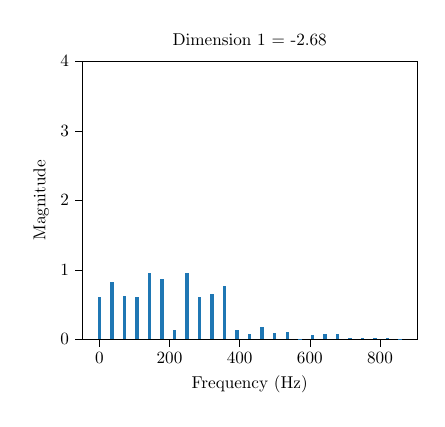
\begin{tikzpicture}[scale=0.62]

\definecolor{darkgray176}{RGB}{176,176,176}
\definecolor{steelblue31119180}{RGB}{31,119,180}

\begin{axis}[
tick align=outside,
tick pos=left,
x grid style={darkgray176},
xlabel={Frequency (Hz)},
xmin=-48.3571428571429, xmax=905.5,
xtick style={color=black},
y grid style={darkgray176},
ylabel={Magnitude},
ymin=0, ymax=4,
title={Dimension 1 = -2.68},
ytick style={color=black}
]
\draw[draw=none,fill=steelblue31119180] (axis cs:-5,0) rectangle (axis cs:5,0.605088098905981);
\draw[draw=none,fill=steelblue31119180] (axis cs:30.7142857142857,0) rectangle (axis cs:40.7142857142857,0.824946037495217);
\draw[draw=none,fill=steelblue31119180] (axis cs:66.4285714285714,0) rectangle (axis cs:76.4285714285714,0.618337924452538);
\draw[draw=none,fill=steelblue31119180] (axis cs:102.142857142857,0) rectangle (axis cs:112.142857142857,0.606547406467815);
\draw[draw=none,fill=steelblue31119180] (axis cs:137.857142857143,0) rectangle (axis cs:147.857142857143,0.952736687378679);
\draw[draw=none,fill=steelblue31119180] (axis cs:173.571428571429,0) rectangle (axis cs:183.571428571429,0.867459344161617);
\draw[draw=none,fill=steelblue31119180] (axis cs:209.285714285714,0) rectangle (axis cs:219.285714285714,0.142171590262196);
\draw[draw=none,fill=steelblue31119180] (axis cs:245,0) rectangle (axis cs:255,0.959357311317153);
\draw[draw=none,fill=steelblue31119180] (axis cs:280.714285714286,0) rectangle (axis cs:290.714285714286,0.614147542320182);
\draw[draw=none,fill=steelblue31119180] (axis cs:316.428571428571,0) rectangle (axis cs:326.428571428571,0.651510920840633);
\draw[draw=none,fill=steelblue31119180] (axis cs:352.142857142857,0) rectangle (axis cs:362.142857142857,0.767848611698322);
\draw[draw=none,fill=steelblue31119180] (axis cs:387.857142857143,0) rectangle (axis cs:397.857142857143,0.130737421425031);
\draw[draw=none,fill=steelblue31119180] (axis cs:423.571428571429,0) rectangle (axis cs:433.571428571429,0.0781024768115382);
\draw[draw=none,fill=steelblue31119180] (axis cs:459.285714285714,0) rectangle (axis cs:469.285714285714,0.174989028847861);
\draw[draw=none,fill=steelblue31119180] (axis cs:495,0) rectangle (axis cs:505,0.0957224281064073);
\draw[draw=none,fill=steelblue31119180] (axis cs:530.714285714286,0) rectangle (axis cs:540.714285714286,0.105812453640171);
\draw[draw=none,fill=steelblue31119180] (axis cs:566.428571428571,0) rectangle (axis cs:576.428571428571,0.00668246230492007);
\draw[draw=none,fill=steelblue31119180] (axis cs:602.142857142857,0) rectangle (axis cs:612.142857142857,0.0584750394429784);
\draw[draw=none,fill=steelblue31119180] (axis cs:637.857142857143,0) rectangle (axis cs:647.857142857143,0.0829703251371982);
\draw[draw=none,fill=steelblue31119180] (axis cs:673.571428571429,0) rectangle (axis cs:683.571428571429,0.0786316144734407);
\draw[draw=none,fill=steelblue31119180] (axis cs:709.285714285714,0) rectangle (axis cs:719.285714285714,0.0183265263662661);
\draw[draw=none,fill=steelblue31119180] (axis cs:745,0) rectangle (axis cs:755,0.0136594016374186);
\draw[draw=none,fill=steelblue31119180] (axis cs:780.714285714286,0) rectangle (axis cs:790.714285714286,0.0150421133154433);
\draw[draw=none,fill=steelblue31119180] (axis cs:816.428571428571,0) rectangle (axis cs:826.428571428571,0.0199113615327003);
\draw[draw=none,fill=steelblue31119180] (axis cs:852.142857142857,0) rectangle (axis cs:862.142857142857,0.00824199961136327);
\end{axis}

\end{tikzpicture}

	\end{subfigure}\hfill
	\begin{subfigure}{0.3\textwidth}
		\centering
		% This file was created with tikzplotlib v0.10.1.
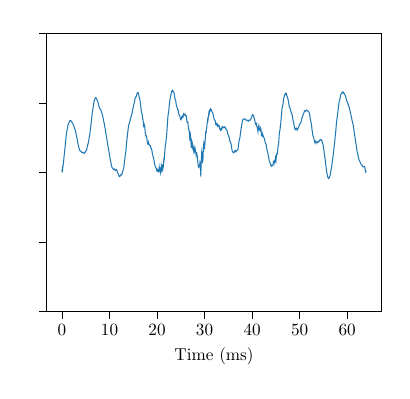
\begin{tikzpicture}[scale=0.62]

\definecolor{darkgray176}{RGB}{176,176,176}
\definecolor{steelblue31119180}{RGB}{31,119,180}

\begin{axis}[
yticklabel={\empty},
tick align=outside,
tick pos=left,
x grid style={darkgray176},
xlabel={Time (ms)},
xmin=-3.2, xmax=67.2,
xtick style={color=black},
y grid style={darkgray176},
% ylabel={Amplitude},
% ymin=-0.15, ymax=0.15,
ymin=-0.1, ymax=0.1,
ytick style={color=black}
]
\addplot [semithick, steelblue31119180]
table {%
0 0
0.0625610948191593 0.00267421979664707
0.125122189638319 0.00195263445792485
0.187683284457478 0.00448575329658223
0.250244379276637 0.00506307051416017
0.312805474095797 0.00741872769886972
0.375366568914956 0.00896099196129705
0.437927663734115 0.0115803680341702
0.500488758553275 0.0133900876509304
0.563049853372434 0.0151754755341063
0.625610948191593 0.0175304286389494
0.688172043010753 0.0195827149455586
0.750733137829912 0.0220035516719752
0.813294232649071 0.0241572310672827
0.875855327468231 0.0260075675241671
0.93841642228739 0.0276190532682753
1.00097751710655 0.029011056083869
1.06353861192571 0.0303319803605681
1.12609970674487 0.0314772311226626
1.18866080156403 0.0323503866813574
1.25122189638319 0.0340090383259345
1.31378299120235 0.0342868589673224
1.37634408602151 0.034962264941104
1.43890518084066 0.0355454103753539
1.50146627565982 0.0360117456070052
1.56402737047898 0.0365307936963797
1.62658846529814 0.0370469956639663
1.6891495601173 0.0372855405697375
1.75171065493646 0.0373638160362883
1.81427174975562 0.0371841114243804
1.87683284457478 0.0371509336557818
1.93939393939394 0.0367688526484099
2.0019550342131 0.0364753106155616
2.06451612903226 0.0361838696464416
2.12707722385142 0.0359691435804378
2.18963831867058 0.0355138606187011
2.25219941348974 0.0352915312351981
2.3147605083089 0.0347998261102134
2.37732160312805 0.0344101194336005
2.43988269794721 0.0336631536920749
2.50244379276637 0.0331262272681571
2.56500488758553 0.0324098647864333
2.62756598240469 0.0318902237095004
2.69012707722385 0.0313611501975318
2.75268817204301 0.030779401080743
2.81524926686217 0.0301372612829257
2.87781036168133 0.0291732079745475
2.94037145650049 0.0278471793837386
3.00293255131965 0.026998937900159
3.06549364613881 0.0261555616457092
3.12805474095797 0.0251639858926059
3.19061583577713 0.0240808387786762
3.25317693059629 0.0226956488526374
3.31573802541544 0.0215881998074457
3.3782991202346 0.0205637725818454
3.44086021505376 0.0194245896512462
3.50342130987292 0.0185915641158907
3.56598240469208 0.0176511272853595
3.62854349951124 0.016837186412203
3.6911045943304 0.0160462343054783
3.75366568914956 0.0156823699676658
3.81622678396872 0.0154439510553638
3.87878787878788 0.0154666042124683
3.94134897360704 0.0152564826052734
4.0039100684262 0.0150434925245487
4.06647116324536 0.01496300729445
4.12903225806452 0.0145273268102638
4.19159335288368 0.0143023412947781
4.25415444770283 0.0141885221670887
4.31671554252199 0.0143579145090496
4.37927663734115 0.0143627272509148
4.44183773216031 0.0143107777445023
4.50439882697947 0.0143003093455631
4.56695992179863 0.0140994674365017
4.62952101661779 0.0139923333422529
4.69208211143695 0.0136977836183788
4.75464320625611 0.013858715826072
4.81720430107527 0.0140708540115626
4.87976539589443 0.0146523808071778
4.94232649071359 0.0149836221114456
5.00488758553275 0.0151687482169821
5.06744868035191 0.0155991362598984
5.13000977517107 0.0159412591371281
5.19257086999022 0.0162529259035227
5.25513196480938 0.017360441337539
5.31769305962854 0.0182014699926999
5.3802541544477 0.0193291187581341
5.44281524926686 0.0200854901912625
5.50537634408602 0.0208316617795537
5.56793743890518 0.0217071624084914
5.63049853372434 0.0229126865049698
5.6930596285435 0.0242266035106175
5.75562072336266 0.0256323526474126
5.81818181818182 0.0267178274013779
5.88074291300098 0.0283921178146279
5.94330400782014 0.0298888944198659
6.0058651026393 0.0314556878562634
6.06842619745846 0.0335125506820042
6.13098729227761 0.0353603800185178
6.19354838709677 0.0371862264169801
6.25610948191593 0.0392754322130921
6.31867057673509 0.0411166230822938
6.38123167155425 0.0428521498174699
6.44379276637341 0.0441375720776246
6.50635386119257 0.0457053787929834
6.56891495601173 0.0472871441710904
6.63147605083089 0.048761960190019
6.69403714565005 0.0498478819788201
6.75659824046921 0.050987220705211
6.81915933528837 0.0516526354504121
6.88172043010753 0.052490993072429
6.94428152492669 0.0530063456738275
7.00684261974585 0.0534649434775289
7.069403714565 0.0537074036634038
7.13196480938416 0.0537072170656885
7.19452590420332 0.0535349667596677
7.25708699902248 0.0530148078673833
7.31964809384164 0.0528068320274003
7.3822091886608 0.0521574912434362
7.44477028347996 0.0515556330096162
7.50733137829912 0.0511457352595857
7.56989247311828 0.0503554332160181
7.63245356793744 0.0496244228928407
7.6950146627566 0.0487227421199297
7.75757575757576 0.0479266882281412
7.82013685239492 0.0471831423031095
7.88269794721408 0.046654381715526
7.94525904203324 0.0460351152001413
8.00782013685239 0.0457550140146898
8.07038123167155 0.0454348212550462
8.13294232649071 0.0452133226112798
8.19550342130987 0.0445972337685198
8.25806451612903 0.0439055550603136
8.32062561094819 0.0433501996252893
8.38318670576735 0.0427576806942476
8.44574780058651 0.0420135908768324
8.50830889540567 0.0413939108542246
8.57086999022483 0.040383708649629
8.63343108504399 0.0394220507029127
8.69599217986315 0.0382373149225439
8.75855327468231 0.0370243414417128
8.82111436950147 0.0361064742824549
8.88367546432062 0.0353182733026156
8.94623655913978 0.034049863776853
9.00879765395894 0.0328304045656122
9.0713587487781 0.0317752120300822
9.13391984359726 0.0303793267955965
9.19648093841642 0.0287503501471361
9.25904203323558 0.0277123870792364
9.32160312805474 0.0264058492072691
9.3841642228739 0.0252075347437624
9.44672531769306 0.0238300412674803
9.50928641251222 0.0225178186025176
9.57184750733138 0.0210519984932589
9.63440860215054 0.0198594470538439
9.6969696969697 0.0187120908363299
9.75953079178886 0.0173988586176962
9.82209188660802 0.0162397695983872
9.88465298142718 0.0150185930283188
9.94721407624633 0.0135728019423499
10.0097751710655 0.0123385272515921
10.0723362658847 0.0110240861762566
10.1348973607038 0.00961095098504398
10.197458455523 0.00825266510554073
10.2600195503421 0.0075971999443259
10.3225806451613 0.00651535481935547
10.3851417399804 0.00549221840684365
10.4477028347996 0.00441473745945787
10.5102639296188 0.00380801213386297
10.5728250244379 0.00333096788884782
10.6353861192571 0.0030224520516448
10.6979472140762 0.00274330640315485
10.7605083088954 0.00251342399357176
10.8230694037146 0.00208306508657695
10.8856304985337 0.00217947526630069
10.9481915933529 0.00227255503649761
11.010752688172 0.00244182444387867
11.0733137829912 0.00224105331533291
11.1358748778104 0.00175680994681599
11.1984359726295 0.00137892175367501
11.2609970674487 0.0013601645838218
11.3235581622678 0.001649708713779
11.386119257087 0.00193779625522951
11.4486803519062 0.00198972274349931
11.5112414467253 0.00166785174057631
11.5738025415445 0.00142994691833548
11.6363636363636 0.00061140903695063
11.6989247311828 -0.000307942650491191
11.761485826002 -0.000503915605132532
11.8240469208211 -0.00113124737401337
11.8866080156403 -0.00155196709236092
11.9491691104594 -0.00214502619049591
12.0117302052786 -0.00279614021264213
12.0742913000978 -0.00304161296212429
12.1368523949169 -0.00297893156076282
12.1994134897361 -0.00285662688817447
12.2619745845552 -0.00236801814582865
12.3245356793744 -0.0021942504504122
12.3870967741935 -0.00160614665477507
12.4496578690127 -0.00156108215123502
12.5122189638319 -0.0018311939707512
12.574780058651 -0.00173706366869012
12.6373411534702 -0.000912511972519309
12.6999022482893 -0.000196902665836721
12.7624633431085 0.000736978850013351
12.8250244379277 0.00106108622335968
12.8875855327468 0.00214182240806542
12.950146627566 0.00270913908383713
13.0127077223851 0.00340024156829129
13.0752688172043 0.00556807706673299
13.1378299120235 0.00725564627725183
13.2003910068426 0.00904701511400187
13.2629521016618 0.0112418273021399
13.3255131964809 0.0124709883655621
13.3880742913001 0.0139866596431938
13.4506353861193 0.0154722398884398
13.5131964809384 0.0179199806613919
13.5757575757576 0.0204215760935437
13.6383186705767 0.0226809065843607
13.7008797653959 0.0248251628578583
13.7634408602151 0.0266148869789416
13.8260019550342 0.0284216282261082
13.8885630498534 0.0303372205931508
13.9511241446725 0.0320307074273087
14.0136852394917 0.0336226689249627
14.0762463343109 0.0342720239436871
14.13880742913 0.0349491323751351
14.2013685239492 0.0356921560931241
14.2639296187683 0.0364141654485394
14.3264907135875 0.0373742953598325
14.3890518084066 0.0380467732554394
14.4516129032258 0.0389382684182736
14.514173998045 0.039927060713123
14.5767350928641 0.0404909389459493
14.6392961876833 0.0411950073032872
14.7018572825024 0.0419001485442311
14.7644183773216 0.0429625525753781
14.8269794721408 0.0438603695558488
14.8895405669599 0.0452642597727849
14.9521016617791 0.0463684541105001
15.0146627565982 0.0474161693220002
15.0772238514174 0.0484258940230367
15.1397849462366 0.048982958699907
15.2023460410557 0.0497803344033506
15.2649071358749 0.051131768807594
15.327468230694 0.0521033428106839
15.3900293255132 0.0531876813511083
15.4525904203324 0.0538189128325307
15.5151515151515 0.0541310210458257
15.5777126099707 0.0543522023735158
15.6402737047898 0.0549303894463785
15.702834799609 0.0555825384328267
15.7653958944282 0.0564133933201826
15.8279569892473 0.056831538196533
15.8905180840665 0.0572587951329534
15.9530791788856 0.057280189141937
16.0156402737048 0.0573616571822736
16.0782013685239 0.056989228402065
16.1407624633431 0.0559466459741952
16.2033235581623 0.0549218033787267
16.2658846529814 0.0539930620970876
16.3284457478006 0.0531750289925382
16.3910068426197 0.0521099569871366
16.4535679374389 0.0510703175386026
16.5161290322581 0.0493302415575712
16.5786901270772 0.0474945895286424
16.6412512218964 0.0456468005039213
16.7038123167155 0.0437111058040274
16.7663734115347 0.0426618811835554
16.8289345063539 0.0419866980607908
16.891495601173 0.0413465699197348
16.9540566959922 0.0398208843953798
17.0166177908113 0.0385363369120443
17.0791788856305 0.0372270050723532
17.1417399804497 0.0345423184062117
17.2043010752688 0.032461166021324
17.266862170088 0.0347551361239813
17.3294232649071 0.0341661413175619
17.3919843597263 0.0338865765739134
17.4545454545455 0.0314861332828348
17.5171065493646 0.0286533663273295
17.5796676441838 0.0271085365361307
17.6422287390029 0.0262852582228411
17.7047898338221 0.0263691197621945
17.7673509286412 0.0262591917002219
17.8299120234604 0.0251460206091317
17.8924731182796 0.023419109804015
17.9550342130987 0.0213664465766848
18.0175953079179 0.0208063320833043
18.080156402737 0.0203971048855275
18.1427174975562 0.0208537711262091
18.2052785923754 0.0216071604644536
18.2678396871945 0.020109887729205
18.3304007820137 0.0199684586124686
18.3929618768328 0.0197349161051673
18.455522971652 0.0194785226671752
18.5180840664712 0.0194128193889807
18.5806451612903 0.0193844509701575
18.6432062561095 0.0188214922176341
18.7057673509286 0.0173547650001878
18.7683284457478 0.0172885383187064
18.830889540567 0.0166502374325417
18.8934506353861 0.0162434242228783
18.9560117302053 0.0150629650757722
19.0185728250244 0.013391328265459
19.0811339198436 0.0127082065490683
19.1436950146628 0.0115744774434661
19.2062561094819 0.0109363535085906
19.2688172043011 0.0104743799254779
19.3313782991202 0.00898958691272917
19.3939393939394 0.00790707682344046
19.4565004887586 0.0066469337168502
19.5190615835777 0.00564898771733657
19.5816226783969 0.0047800187185363
19.644183773216 0.00409872611968224
19.7067448680352 0.00366864474681465
19.7693059628544 0.00332232838895314
19.8318670576735 0.00288059430803197
19.8944281524927 0.00273982084238809
19.9569892473118 0.000845879196159301
20.019550342131 0.000760033273321092
20.0821114369501 0.00095205489120001
20.1446725317693 0.0019063416846599
20.2072336265885 0.00162790942926211
20.2697947214076 0.000875847490608168
20.3323558162268 0.000575767573286014
20.3949169110459 0.00160671152786251
20.4574780058651 0.00388647337332149
20.5200391006843 0.00233205468489453
20.5826001955034 0.00152916488540837
20.6451612903226 0.00328123563479993
20.7077223851417 0.00326864568303582
20.7702834799609 -0.00020999720325568
20.8328445747801 0.000763068778598764
20.8954056695992 0.00438050786442945
20.9579667644184 0.0029384327555332
21.0205278592375 0.000206796255760179
21.0830889540567 0.00278985447351359
21.1456500488759 0.00508365880075263
21.208211143695 0.00488976083280753
21.2707722385142 0.00338998097718811
21.3333333333333 0.00464094616472721
21.3958944281525 0.00786668587683582
21.4584555229717 0.0097706981789856
21.5210166177908 0.00937353533384038
21.58357771261 0.0119085969113884
21.6461388074291 0.0154543465107155
21.7086999022483 0.0183054468160238
21.7712609970674 0.0201115640770655
21.8338220918866 0.0206162288205977
21.8963831867058 0.0229037094675551
21.9589442815249 0.0247902948616886
22.0215053763441 0.0266693644826451
22.0840664711632 0.030081022257679
22.1466275659824 0.0328973525659867
22.2091886608016 0.0361175192438088
22.2717497556207 0.0395221697477913
22.3343108504399 0.041304173204731
22.396871945259 0.0427716355006104
22.4594330400782 0.0439727842436333
22.5219941348974 0.04629844911615
22.5845552297165 0.0490542658088494
22.6471163245357 0.0508796651724759
22.7096774193548 0.0520982259223538
22.772238514174 0.0532420461729737
22.8347996089932 0.0545685695609914
22.8973607038123 0.0551733477560044
22.9599217986315 0.0559879976305619
23.0224828934506 0.0578949249723702
23.0850439882698 0.0583804640755101
23.147605083089 0.0584930904439031
23.2101661779081 0.0588970233377648
23.2727272727273 0.0583844416859475
23.3352883675464 0.0586766382225972
23.3978494623656 0.0583387540593263
23.4604105571848 0.0581928974350701
23.5229716520039 0.0575271020438577
23.5855327468231 0.0569285704942742
23.6480938416422 0.0559307399787599
23.7106549364614 0.0543003477199861
23.7732160312805 0.0534002241184198
23.8357771260997 0.0520780251260377
23.8983382209189 0.0516900767864457
23.960899315738 0.0508313895888692
24.0234604105572 0.049175866521742
24.0860215053763 0.0479400197584783
24.1485826001955 0.0473373903895665
24.2111436950147 0.046511578878874
24.2737047898338 0.0462514713264543
24.336265884653 0.0451448697848054
24.3988269794721 0.0451817311991083
24.4613880742913 0.0443530065114023
24.5239491691105 0.0426578202784673
24.5865102639296 0.0416546216196329
24.6490713587488 0.0413088361156389
24.7116324535679 0.041108225174576
24.7741935483871 0.0408650341654016
24.8367546432063 0.0398515648812143
24.8993157380254 0.038847956440447
24.9618768328446 0.0380346358281252
25.0244379276637 0.0378304746854078
25.0869990224829 0.0382387661689188
25.1495601173021 0.0390100164114992
25.2121212121212 0.0399538556283171
25.2746823069404 0.040413034577305
25.3372434017595 0.0400065938966715
25.3998044965787 0.0394734188400843
25.4623655913978 0.0394740778832666
25.524926686217 0.0411028750513918
25.5874877810362 0.0420756560485384
25.6500488758553 0.0417780720757162
25.7126099706745 0.0412677814774324
25.7751710654936 0.041175230032057
25.8377321603128 0.0413646532599527
25.900293255132 0.0417800190697405
25.9628543499511 0.0412614583269941
26.0254154447703 0.0406542915544989
26.0879765395894 0.0408050164667742
26.1505376344086 0.0405792076621325
26.2130987292278 0.0390043036023543
26.2756598240469 0.0368666124866068
26.3382209188661 0.0360929401389315
26.4007820136852 0.0362097313818781
26.4633431085044 0.036331480986212
26.5259042033236 0.0345905183860896
26.5884652981427 0.031986461903168
26.6510263929619 0.031094742556515
26.713587487781 0.0309626471546214
26.7761485826002 0.0293936625811274
26.8387096774194 0.0263035376706431
26.9012707722385 0.0239715223744118
26.9638318670577 0.0245473122229674
27.0263929618768 0.026747274624943
27.088954056696 0.0248879576893933
27.1515151515152 0.0209304007955573
27.2140762463343 0.0176937769814408
27.2766373411535 0.0196157470454743
27.3391984359726 0.0221516430880492
27.4017595307918 0.0213706412317117
27.4643206256109 0.0188635372914527
27.5268817204301 0.0167689943505872
27.5894428152493 0.0163053760518077
27.6520039100684 0.0177176835621732
27.7145650048876 0.0165713070960076
27.7771260997067 0.0141103166617082
27.8396871945259 0.0146560471428454
27.9022482893451 0.0159809314031318
27.9648093841642 0.0179326702619403
28.0273704789834 0.0170464531690581
28.0899315738025 0.0151981798565982
28.1524926686217 0.0144559601349128
28.2150537634409 0.0127864169377473
28.27761485826 0.0140569939160627
28.3401759530792 0.0141271333486017
28.4027370478983 0.0123410444444488
28.4652981427175 0.0116867676508392
28.5278592375367 0.00907893372355493
28.5904203323558 0.00709933834013876
28.652981427175 0.00512608153816542
28.7155425219941 0.00378594341035113
28.7781036168133 0.00356751068050036
28.8406647116325 0.00437589089148555
28.9032258064516 0.00465376368693767
28.9657869012708 0.00537902522078357
29.0283479960899 0.00695361941506611
29.0909090909091 0.00594923797656189
29.1534701857282 0.0013902217881683
29.2160312805474 -0.00304396178496898
29.2785923753666 0.00566547975228154
29.3411534701857 0.0108653606896089
29.4037145650049 0.014694018147427
29.466275659824 0.0133876833037809
29.5288367546432 0.0101675867400736
29.5913978494624 0.00803752129356707
29.6539589442815 0.00901241266766776
29.7165200391007 0.0144135524133696
29.7790811339198 0.0189351138667015
29.841642228739 0.0207817511103195
29.9042033235582 0.0193139174816545
29.9667644183773 0.0165541066113543
30.0293255131965 0.0189539923051323
30.0918866080156 0.0218169781491379
30.1544477028348 0.0246398184022421
30.217008797654 0.0282433863696465
30.2795698924731 0.0278777189913296
30.3421309872923 0.0289339464911617
30.4046920821114 0.0309737586632065
30.4672531769306 0.0327821483513302
30.5298142717498 0.0346808726039013
30.5923753665689 0.0366036100777363
30.6549364613881 0.0380971568562855
30.7174975562072 0.0375351592286591
30.7800586510264 0.0395417567124028
30.8426197458456 0.0406106800015721
30.9051808406647 0.0431468461276936
30.9677419354839 0.0440592289932313
31.030303030303 0.0431223926557736
31.0928641251222 0.044251091953072
31.1554252199413 0.044091906240128
31.2179863147605 0.0447321454734921
31.2805474095797 0.0457030936278119
31.3431085043988 0.0453781697494893
31.405669599218 0.0451644942153496
31.4682306940371 0.0443997886414227
31.5307917888563 0.0437652633369756
31.5933528836755 0.0434029524452176
31.6559139784946 0.043035791225491
31.7184750733138 0.0426897188741441
31.7810361681329 0.0420002157354722
31.8435972629521 0.0409411973268056
31.9061583577713 0.039571873412148
31.9687194525904 0.0386384047371202
32.0312805474096 0.0383785877573438
32.0938416422287 0.0375490882092557
32.1564027370479 0.0375753101944661
32.2189638318671 0.0374420748537412
32.2815249266862 0.0360706945788388
32.3440860215054 0.0350615131037851
32.4066471163245 0.0339929430507932
32.4692082111437 0.0340246002345491
32.5317693059629 0.0349592938636842
32.594330400782 0.0352224107842641
32.6568914956012 0.034789714257607
32.7194525904203 0.0336865213565812
32.7820136852395 0.0331596681176305
32.8445747800587 0.0334299338702932
32.9071358748778 0.0338081808875471
32.969696969697 0.033365224911408
33.0322580645161 0.0329333330474554
33.0948191593353 0.0332109972266508
33.1573802541544 0.0320883396838155
33.2199413489736 0.0309007317046266
33.2825024437928 0.0308718603716131
33.3450635386119 0.030459921162499
33.4076246334311 0.0313069512603307
33.4701857282502 0.0315470496121565
33.5327468230694 0.0310009366223627
33.5953079178886 0.0306450518563696
33.6578690127077 0.0318058445295892
33.7204301075269 0.0329603675392366
33.782991202346 0.0327633887562147
33.8455522971652 0.032416258422423
33.9081133919844 0.0322558210119387
33.9706744868035 0.0320788991918837
34.0332355816227 0.0323125378903318
34.0957966764418 0.0326428515973154
34.158357771261 0.0326298984297472
34.2209188660802 0.032318359519467
34.2834799608993 0.0326219256421076
34.3460410557185 0.0323100589062811
34.4086021505376 0.0318218369277254
34.4711632453568 0.0310809285082251
34.533724340176 0.0310058263226076
34.5962854349951 0.0309875087370096
34.6588465298143 0.0306313110466315
34.7214076246334 0.0300611066044775
34.7839687194526 0.0293552047379118
34.8465298142717 0.0284407946480509
34.9090909090909 0.0275458454747092
34.9716520039101 0.0268777255023505
35.0342130987292 0.0267992109508196
35.0967741935484 0.0259139400816733
35.1593352883675 0.0252057173592516
35.2218963831867 0.0244404716182314
35.2844574780059 0.0227533189738251
35.347018572825 0.0225678494751803
35.4095796676442 0.0221244483268506
35.4721407624633 0.0217717170190951
35.5347018572825 0.0210364933925902
35.5972629521017 0.0201191887521674
35.6598240469208 0.0188929513752286
35.72238514174 0.0170571037685591
35.7849462365591 0.0159716786396119
35.8475073313783 0.0150278387563931
35.9100684261975 0.01489631146127
35.9726295210166 0.0146592597305076
36.0351906158358 0.0141087751125485
36.0977517106549 0.014124936951308
36.1603128054741 0.014254863567847
36.2228739002933 0.0143559359483792
36.2854349951124 0.0151110854862897
36.3479960899316 0.0150740762566192
36.4105571847507 0.0157257782082316
36.4731182795699 0.0156458070681941
36.5356793743891 0.0150090577654388
36.5982404692082 0.0147384244052808
36.6608015640274 0.015120394850188
36.7233626588465 0.0154524166027734
36.7859237536657 0.0158782299892032
36.8484848484849 0.0158998847685077
36.911045943304 0.0161424008337371
36.9736070381232 0.0162015636984117
37.0361681329423 0.0167102424422405
37.0987292277615 0.0182204747960365
37.1612903225806 0.0200580241939714
37.2238514173998 0.0217561341133897
37.286412512219 0.0231641612652023
37.3489736070381 0.0238318093219373
37.4115347018573 0.0247525442883241
37.4740957966764 0.025644510700381
37.5366568914956 0.0275202778514879
37.5992179863148 0.0292770331534298
37.6617790811339 0.0308391401746318
37.7243401759531 0.0322980790063083
37.7869012707722 0.0334602463116482
37.8494623655914 0.0347619480904072
37.9120234604106 0.0359631676139457
37.9745845552297 0.0368996791847465
38.0371456500489 0.0378674757434738
38.099706744868 0.0381146148939636
38.1622678396872 0.0383059976245563
38.2248289345064 0.0384774612279232
38.2873900293255 0.0383171840049217
38.3499511241447 0.0384484256489361
38.4125122189638 0.0384597241212109
38.475073313783 0.0384790841216915
38.5376344086022 0.0383175552011498
38.6001955034213 0.0377998699016235
38.6627565982405 0.0377321959448612
38.7253176930596 0.0376487938124588
38.7878787878788 0.0376734474504536
38.8504398826979 0.0375150216967304
38.9130009775171 0.0375846544897888
38.9755620723363 0.0374904452902306
39.0381231671554 0.0374442960608128
39.1006842619746 0.0372936971420067
39.1632453567937 0.0369457174420269
39.2258064516129 0.0368236430710362
39.2883675464321 0.0373380606245697
39.3509286412512 0.0374558800476387
39.4134897360704 0.0376636466049641
39.4760508308895 0.0376178475528344
39.5386119257087 0.0375941767250775
39.6011730205279 0.0375067810814751
39.663734115347 0.0377316429959801
39.7262952101662 0.0381126951568287
39.7888563049853 0.0388838746188935
39.8514173998045 0.0394202564840268
39.9139784946237 0.0397456081043328
39.9765395894428 0.040315290339444
40.039100684262 0.0412298003457421
40.1016617790811 0.0414068146316537
40.1642228739003 0.0410492199574136
40.2267839687195 0.0411880649189271
40.2893450635386 0.0409462820694856
40.3519061583578 0.0401449904195374
40.4144672531769 0.0390465733406743
40.4770283479961 0.0386799932662343
40.5395894428152 0.0376865399668206
40.6021505376344 0.0366314517394189
40.6647116324536 0.0358175872347135
40.7272727272727 0.0348084318366918
40.7898338220919 0.0344157486531304
40.852394916911 0.0347675312081041
40.9149560117302 0.0350688882335977
40.9775171065494 0.0333061736634225
41.0400782013685 0.032600074356471
41.1026392961877 0.0321379145088434
41.1652003910068 0.0307046050080194
41.227761485826 0.0294969624176053
41.2903225806452 0.0325823667188806
41.3528836754643 0.0329074016895112
41.4154447702835 0.0337845209570836
41.4780058651026 0.0325840122975912
41.5405669599218 0.0306703675909738
41.603128054741 0.0305694714953298
41.6656891495601 0.030171353113223
41.7282502443793 0.031143564140954
41.7908113391984 0.0318894302554407
41.8533724340176 0.0306748176468782
41.9159335288368 0.0292985609669752
41.9784946236559 0.0267994198347292
42.0410557184751 0.0260753441394424
42.1036168132942 0.026039359364604
42.1661779081134 0.0267842792553549
42.2287390029325 0.0277295210439701
42.2913000977517 0.0265493077660236
42.3538611925709 0.0261299217016029
42.41642228739 0.0255084721661034
42.4789833822092 0.0248335181486921
42.5415444770283 0.0245418480742187
42.6041055718475 0.0241732470297918
42.6666666666667 0.0232807192951441
42.7292277614858 0.0216111164933338
42.791788856305 0.0214149535488873
42.8543499511241 0.0207516336130781
42.9169110459433 0.0204178342306194
42.9794721407625 0.0192357806592655
43.0420332355816 0.0175879018878307
43.1045943304008 0.0168795692693453
43.1671554252199 0.0155753857808466
43.2297165200391 0.0148914705776224
43.2922776148583 0.0144289083986426
43.3548387096774 0.0130980704580584
43.4173998044966 0.0120939013611012
43.4799608993157 0.0108472363548108
43.5425219941349 0.00960976536497692
43.6050830889541 0.00849363266809944
43.6676441837732 0.00765429090304284
43.7302052785924 0.00705099843245797
43.7927663734115 0.00663502100866037
43.8553274682307 0.00606322959283929
43.9178885630498 0.00568777587690836
43.980449657869 0.00445893265940576
44.0430107526882 0.00439443637526804
44.1055718475073 0.00446561516380031
44.1681329423265 0.00513564554368121
44.2306940371457 0.00521406070861823
44.2932551319648 0.00499794883462341
44.355816226784 0.00488837840051945
44.4183773216031 0.00564268229753216
44.4809384164223 0.00737928005366906
44.5434995112414 0.00707713632552155
44.6060606060606 0.0070919179442254
44.6686217008798 0.00851020454551992
44.7311827956989 0.00866406987751684
44.7937438905181 0.00704828820729361
44.8563049853372 0.00816068935953627
44.9188660801564 0.0108787558229962
44.9814271749756 0.010371167922824
45.0439882697947 0.00914865583618366
45.1065493646139 0.0114646889706336
45.169110459433 0.0132357996787406
45.2316715542522 0.0134156004817954
45.2942326490714 0.0132334446288711
45.3567937438905 0.0144499974472781
45.4193548387097 0.0173056817222987
45.4819159335288 0.019130442198639
45.544477028348 0.0196244097710792
45.6070381231672 0.021854941905244
45.6695992179863 0.025132772351596
45.7321603128055 0.0278786127168762
45.7947214076246 0.0295117591614248
45.8572825024438 0.0303778906852619
45.919843597263 0.0322564648426086
45.9824046920821 0.0339553831500217
46.0449657869013 0.0358612972128688
46.1075268817204 0.0385077691847278
46.1700879765396 0.0408807266175834
46.2326490713588 0.0432648152178508
46.2952101661779 0.0456662636709091
46.3577712609971 0.046847217615224
46.4203323558162 0.0477867429458763
46.4828934506354 0.0485950412004749
46.5454545454545 0.0505165232514793
46.6080156402737 0.0525513137322018
46.6705767350929 0.0537294811593735
46.733137829912 0.0543446789913513
46.7956989247312 0.0549502618490688
46.8582600195503 0.0558704715495235
46.9208211143695 0.0559133530329487
46.9833822091887 0.0559761648194706
47.0459433040078 0.0569916450940182
47.108504398827 0.0570250419883434
47.1710654936461 0.0568927230690319
47.2336265884653 0.056640900562236
47.2961876832845 0.0551848630653011
47.3587487781036 0.0547586485437634
47.4213098729228 0.0541026841936486
47.4838709677419 0.0536307193819554
47.5464320625611 0.0527246055135891
47.6089931573803 0.0517289356664479
47.6715542521994 0.0508142424545243
47.7341153470186 0.0493116723564713
47.7966764418377 0.0481130375179989
47.8592375366569 0.0468085671821473
47.9217986314761 0.0465829856202137
47.9843597262952 0.0462157163670685
48.0469208211144 0.0452095076736729
48.1094819159335 0.0442796264532025
48.1720430107527 0.0438324161955426
48.2346041055718 0.0430557673409188
48.297165200391 0.0426278280099728
48.3597262952102 0.0418391911711686
48.4222873900293 0.041594998058904
48.4848484848485 0.0406052067198537
48.5474095796676 0.0389845076664365
48.6099706744868 0.0375579707433751
48.672531769306 0.0365544479842847
48.7350928641251 0.0357116901280244
48.7976539589443 0.0348651324756596
48.8602150537634 0.0336367660953153
48.9227761485826 0.0324083252091649
48.9853372434018 0.0313928293670552
49.0478983382209 0.0309147811563046
49.1104594330401 0.030692954686992
49.1730205278592 0.0309709876699269
49.2355816226784 0.031597696648927
49.2981427174976 0.0318774469906896
49.3607038123167 0.0314093900085195
49.4232649071359 0.0308339031047223
49.485826001955 0.0304353637648118
49.5483870967742 0.031060064812341
49.6109481915934 0.0315283893490117
49.6735092864125 0.031664160946029
49.7360703812317 0.0318912170565198
49.7986314760508 0.0325307298582757
49.86119257087 0.0333566375601152
49.9237536656891 0.0340274055474752
49.9863147605083 0.0343475082337507
50.0488758553275 0.0348904801374219
50.1114369501466 0.0352367120098508
50.1739980449658 0.0354705928521684
50.2365591397849 0.0357889670037454
50.2991202346041 0.0362658038287481
50.3616813294233 0.0370228979681944
50.4242424242424 0.0380117535929788
50.4868035190616 0.0389377374933962
50.5493646138807 0.0395894841484922
50.6119257086999 0.0399620687244924
50.6744868035191 0.0408489817802595
50.7370478983382 0.0415870843897642
50.7996089931574 0.0421664896325544
50.8621700879765 0.0424486465118498
50.9247311827957 0.04317258929293
50.9872922776149 0.0436714500341772
51.049853372434 0.0439890157977594
51.1124144672532 0.044358433877006
51.1749755620723 0.0441271898738188
51.2375366568915 0.0438700103995737
51.3000977517107 0.0442643841985296
51.3626588465298 0.0446783232221331
51.425219941349 0.0449076517597059
51.4877810361681 0.0448242272755617
51.5503421309873 0.0448317967322477
51.6129032258064 0.0444544803711676
51.6754643206256 0.0442608096459307
51.7380254154448 0.0440060031816057
51.8005865102639 0.0440069565227217
51.8631476050831 0.0439781410690626
51.9257086999022 0.0437708097043013
51.9882697947214 0.0431585281082262
52.0508308895406 0.0425149987771277
52.1133919843597 0.0415439978023428
52.1759530791789 0.0401725728239569
52.238514173998 0.0387360111447024
52.3010752688172 0.0377038967825713
52.3636363636364 0.0366723598404364
52.4261974584555 0.0354431589950652
52.4887585532747 0.0341393890137896
52.5513196480938 0.0325012071730017
52.613880742913 0.0306788693315997
52.6764418377322 0.0291148989988475
52.7390029325513 0.0275694079686208
52.8015640273705 0.0265256427610812
52.8641251221896 0.0256399043680024
52.9266862170088 0.0253011354482856
52.989247311828 0.0243811560494284
53.0518084066471 0.0233437759894605
53.1143695014663 0.0225893578046927
53.1769305962854 0.0217172744632029
53.2394916911046 0.0211648024028697
53.3020527859238 0.0224554698717647
53.3646138807429 0.0222937956649013
53.4271749755621 0.0224200454199157
53.4897360703812 0.0216772929817176
53.5522971652004 0.0212178265189757
53.6148582600196 0.0211791725736385
53.6774193548387 0.0211344315039535
53.7399804496579 0.0214040229790721
53.802541544477 0.0220809991627145
53.8651026392962 0.0223197899376455
53.9276637341153 0.0223311759542423
53.9902248289345 0.0219567615943046
54.0527859237537 0.0220094107888923
54.1153470185728 0.0223439676015258
54.177908113392 0.0227976033185497
54.2404692082111 0.0232850162427097
54.3030303030303 0.0231732385741039
54.3655913978495 0.0234766053937135
54.4281524926686 0.0236280772266937
54.4907135874878 0.0235211834136692
54.5532746823069 0.0233881529639106
54.6158357771261 0.0231276766077514
54.6783968719453 0.0227126081547867
54.7409579667644 0.0217724376825119
54.8035190615836 0.0213462827656189
54.8660801564027 0.0205169620314651
54.9286412512219 0.020012508963079
54.9912023460411 0.0188231631359659
55.0537634408602 0.0171258385863996
55.1163245356794 0.0157880976828924
55.1788856304985 0.0139106013306862
55.2414467253177 0.0122885611727615
55.3040078201369 0.0112943628152882
55.366568914956 0.0093972099688221
55.4291300097752 0.00770373364413414
55.4916911045943 0.00584246838175831
55.5542521994135 0.00412534391425572
55.6168132942326 0.00245839351913796
55.6793743890518 0.000780038147771465
55.741935483871 -0.000622202431963335
55.8044965786901 -0.00163171173256339
55.8670576735093 -0.00270341847998656
55.9296187683284 -0.00340635501547468
55.9921798631476 -0.00384208765372503
56.0547409579668 -0.00413895264551961
56.1173020527859 -0.00444098088966786
56.1798631476051 -0.00418070636558568
56.2424242424242 -0.00360199775208126
56.3049853372434 -0.00304885953118549
56.3675464320626 -0.00252012568703495
56.4301075268817 -0.0017775341027206
56.4926686217009 -0.000825290630989413
56.55522971652 0.000563787831720022
56.6177908113392 0.00183773806040063
56.6803519061584 0.00313017317954221
56.7429130009775 0.00412363140049044
56.8054740957967 0.00566291729332415
56.8680351906158 0.00711228026628844
56.930596285435 0.0089067299181153
56.9931573802542 0.0104306080102746
57.0557184750733 0.0119805407827813
57.1182795698925 0.0143055500042054
57.1808406647116 0.0158458994674193
57.2434017595308 0.0175163397931458
57.3059628543499 0.0196888505309121
57.3685239491691 0.0215753390674979
57.4310850439883 0.023990589721112
57.4936461388074 0.0260414846317946
57.5562072336266 0.0279752023987844
57.6187683284457 0.0300400056807963
57.6813294232649 0.03277259705113
57.7438905180841 0.0352639255832193
57.8064516129032 0.0372064629749906
57.8690127077224 0.0387646770678308
57.9315738025415 0.0404650743154924
57.9941348973607 0.0420708640907342
58.0566959921799 0.0439263153711984
58.119257086999 0.0457073502526605
58.1818181818182 0.0474987526170232
58.2443792766373 0.0490374536392801
58.3069403714565 0.0505239223662622
58.3695014662757 0.0515297504136464
58.4320625610948 0.0522976404443777
58.494623655914 0.0528898979386976
58.5571847507331 0.0540614753273313
58.6197458455523 0.0552708644124944
58.6823069403715 0.0560077898302648
58.7448680351906 0.0564124975845087
58.8074291300098 0.0568147131195428
58.8699902248289 0.0571315971550005
58.9325513196481 0.0569640071871431
58.9951124144673 0.0570515101977632
59.0576735092864 0.0578324908986032
59.1202346041056 0.0576970315595701
59.1827956989247 0.057722884741041
59.2453567937439 0.0576931007119043
59.307917888563 0.0567069899596689
59.3704789833822 0.0566763006849897
59.4330400782014 0.05626079637306
59.4956011730205 0.0559517869348925
59.5581622678397 0.0556505410017069
59.6207233626588 0.055134919513006
59.683284457478 0.0544264769984568
59.7458455522972 0.053288635172365
59.8084066471163 0.0526271909202211
59.8709677419355 0.0517917160064943
59.9335288367546 0.0514830865479372
59.9960899315738 0.051134827451185
60.058651026393 0.0505215214002779
60.1212121212121 0.0497802963311022
60.1837732160313 0.0491487996876677
60.2463343108504 0.0484007759636973
60.3088954056696 0.0478875684631098
60.3714565004888 0.0473363406497362
60.4340175953079 0.0468872565710562
60.4965786901271 0.0460121147662314
60.5591397849462 0.0450108979618357
60.6217008797654 0.0438298725706042
60.6842619745846 0.0428822552430228
60.7468230694037 0.0419466333502024
60.8093841642229 0.0411196371971949
60.871945259042 0.0403209532504557
60.9345063538612 0.039276586408533
60.9970674486804 0.0380582447843817
61.0596285434995 0.0371007740639609
61.1221896383187 0.0360698294429835
61.1847507331378 0.0353156627153109
61.247311827957 0.0343963464181269
61.3098729227762 0.0335445323811511
61.3724340175953 0.031944404380762
61.4349951124145 0.0303682355849274
61.4975562072336 0.0286385904167317
61.5601173020528 0.0272719170461215
61.6226783968719 0.0258196607188395
61.6852394916911 0.0243035696796483
61.7478005865103 0.0227989208696088
61.8103616813294 0.021500640103588
61.8729227761486 0.0203646199444522
61.9354838709677 0.0187503377035741
61.9980449657869 0.0170625145069141
62.0606060606061 0.0159145622429523
62.1231671554252 0.0145981244120168
62.1857282502444 0.0137994386026324
62.2482893450635 0.012727528826888
62.3108504398827 0.0117746551146955
62.3734115347019 0.0107542865928754
62.435972629521 0.00994687242832177
62.4985337243402 0.00900293568755525
62.5610948191593 0.00859378858351987
62.6236559139785 0.00813819083475298
62.6862170087977 0.00771863340697855
62.7487781036168 0.00717838961205
62.811339198436 0.00671188235064406
62.8739002932551 0.00621034618456168
62.9364613880743 0.00593350649076647
62.9990224828935 0.0054801793064365
63.0615835777126 0.00537889578060146
63.1241446725318 0.00507545192613979
63.1867057673509 0.0048174845529966
63.2492668621701 0.00437471670401761
63.3118279569892 0.00417060399007413
63.3743890518084 0.00395582949529645
63.4369501466276 0.00400284605095289
63.4995112414467 0.00400681501456544
63.5620723362659 0.00419773767180632
63.624633431085 0.00398296317702864
63.6871945259042 0.00392700898354529
63.7497556207234 0.0032044941848936
63.8123167155425 0.00166316802922057
63.8748778103617 0.000470869909545896
63.9374389051808 0.000761237328659056
64 0
};
\end{axis}

\end{tikzpicture}

	\end{subfigure}\hfill
	\begin{subfigure}{0.3\textwidth}
		\centering
		% This file was created with tikzplotlib v0.10.1.
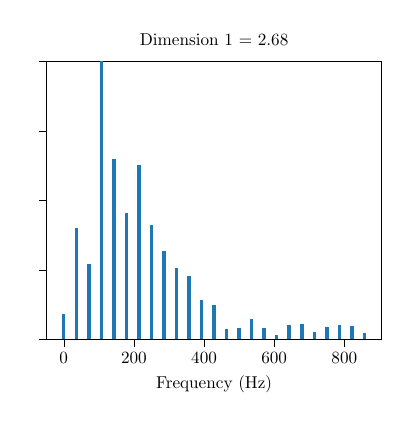
\begin{tikzpicture}[scale=0.62]

\definecolor{darkgray176}{RGB}{176,176,176}
\definecolor{steelblue31119180}{RGB}{31,119,180}

\begin{axis}[
yticklabel={\empty},
tick align=outside,
tick pos=left,
x grid style={darkgray176},
xlabel={Frequency (Hz)},
xmin=-48.3571428571429, xmax=905.5,
xtick style={color=black},
y grid style={darkgray176},
%ylabel={Magnitude},
ymin=0, ymax=4,
title={Dimension 1 = 2.68},
ytick style={color=black}
]
\draw[draw=none,fill=steelblue31119180] (axis cs:-5,0) rectangle (axis cs:5,0.363293109461665);
\draw[draw=none,fill=steelblue31119180] (axis cs:30.7142857142857,0) rectangle (axis cs:40.7142857142857,1.59671692845371);
\draw[draw=none,fill=steelblue31119180] (axis cs:66.4285714285714,0) rectangle (axis cs:76.4285714285714,1.08375129075336);
\draw[draw=none,fill=steelblue31119180] (axis cs:102.142857142857,0) rectangle (axis cs:112.142857142857,5.72028640718505);
\draw[draw=none,fill=steelblue31119180] (axis cs:137.857142857143,0) rectangle (axis cs:147.857142857143,2.60109171070077);
\draw[draw=none,fill=steelblue31119180] (axis cs:173.571428571429,0) rectangle (axis cs:183.571428571429,1.82230187959835);
\draw[draw=none,fill=steelblue31119180] (axis cs:209.285714285714,0) rectangle (axis cs:219.285714285714,2.50466396839656);
\draw[draw=none,fill=steelblue31119180] (axis cs:245,0) rectangle (axis cs:255,1.64154431128106);
\draw[draw=none,fill=steelblue31119180] (axis cs:280.714285714286,0) rectangle (axis cs:290.714285714286,1.2779936763853);
\draw[draw=none,fill=steelblue31119180] (axis cs:316.428571428571,0) rectangle (axis cs:326.428571428571,1.02566988726104);
\draw[draw=none,fill=steelblue31119180] (axis cs:352.142857142857,0) rectangle (axis cs:362.142857142857,0.906444113984638);
\draw[draw=none,fill=steelblue31119180] (axis cs:387.857142857143,0) rectangle (axis cs:397.857142857143,0.567573738688084);
\draw[draw=none,fill=steelblue31119180] (axis cs:423.571428571429,0) rectangle (axis cs:433.571428571429,0.497884322563813);
\draw[draw=none,fill=steelblue31119180] (axis cs:459.285714285714,0) rectangle (axis cs:469.285714285714,0.143370970638671);
\draw[draw=none,fill=steelblue31119180] (axis cs:495,0) rectangle (axis cs:505,0.158030205491621);
\draw[draw=none,fill=steelblue31119180] (axis cs:530.714285714286,0) rectangle (axis cs:540.714285714286,0.287791882784369);
\draw[draw=none,fill=steelblue31119180] (axis cs:566.428571428571,0) rectangle (axis cs:576.428571428571,0.164560600100172);
\draw[draw=none,fill=steelblue31119180] (axis cs:602.142857142857,0) rectangle (axis cs:612.142857142857,0.0653538748355305);
\draw[draw=none,fill=steelblue31119180] (axis cs:637.857142857143,0) rectangle (axis cs:647.857142857143,0.209706204538538);
\draw[draw=none,fill=steelblue31119180] (axis cs:673.571428571429,0) rectangle (axis cs:683.571428571429,0.216581742305538);
\draw[draw=none,fill=steelblue31119180] (axis cs:709.285714285714,0) rectangle (axis cs:719.285714285714,0.104565114650486);
\draw[draw=none,fill=steelblue31119180] (axis cs:745,0) rectangle (axis cs:755,0.18370350932939);
\draw[draw=none,fill=steelblue31119180] (axis cs:780.714285714286,0) rectangle (axis cs:790.714285714286,0.206670350113575);
\draw[draw=none,fill=steelblue31119180] (axis cs:816.428571428571,0) rectangle (axis cs:826.428571428571,0.196489132073225);
\draw[draw=none,fill=steelblue31119180] (axis cs:852.142857142857,0) rectangle (axis cs:862.142857142857,0.0885177801919891);
\end{axis}

\end{tikzpicture}

	\end{subfigure}
	
	\vspace{0.5cm} % Adjust vertical spacing between rows
	
	\begin{subfigure}{0.36\textwidth}
		\centering
		% This file was created with tikzplotlib v0.10.1.
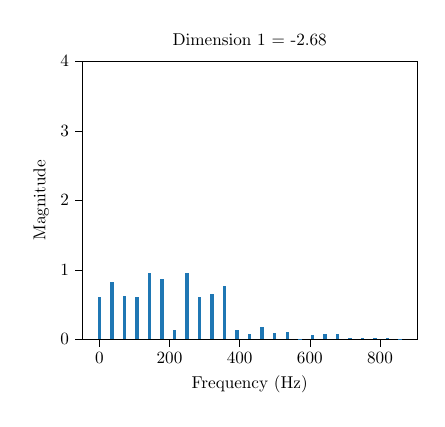
\begin{tikzpicture}[scale=0.62]

\definecolor{darkgray176}{RGB}{176,176,176}
\definecolor{steelblue31119180}{RGB}{31,119,180}

\begin{axis}[
tick align=outside,
tick pos=left,
x grid style={darkgray176},
xlabel={Frequency (Hz)},
xmin=-48.3571428571429, xmax=905.5,
xtick style={color=black},
y grid style={darkgray176},
ylabel={Magnitude},
ymin=0, ymax=4,
title={Dimension 1 = -2.68},
ytick style={color=black}
]
\draw[draw=none,fill=steelblue31119180] (axis cs:-5,0) rectangle (axis cs:5,0.605088098905981);
\draw[draw=none,fill=steelblue31119180] (axis cs:30.7142857142857,0) rectangle (axis cs:40.7142857142857,0.824946037495217);
\draw[draw=none,fill=steelblue31119180] (axis cs:66.4285714285714,0) rectangle (axis cs:76.4285714285714,0.618337924452538);
\draw[draw=none,fill=steelblue31119180] (axis cs:102.142857142857,0) rectangle (axis cs:112.142857142857,0.606547406467815);
\draw[draw=none,fill=steelblue31119180] (axis cs:137.857142857143,0) rectangle (axis cs:147.857142857143,0.952736687378679);
\draw[draw=none,fill=steelblue31119180] (axis cs:173.571428571429,0) rectangle (axis cs:183.571428571429,0.867459344161617);
\draw[draw=none,fill=steelblue31119180] (axis cs:209.285714285714,0) rectangle (axis cs:219.285714285714,0.142171590262196);
\draw[draw=none,fill=steelblue31119180] (axis cs:245,0) rectangle (axis cs:255,0.959357311317153);
\draw[draw=none,fill=steelblue31119180] (axis cs:280.714285714286,0) rectangle (axis cs:290.714285714286,0.614147542320182);
\draw[draw=none,fill=steelblue31119180] (axis cs:316.428571428571,0) rectangle (axis cs:326.428571428571,0.651510920840633);
\draw[draw=none,fill=steelblue31119180] (axis cs:352.142857142857,0) rectangle (axis cs:362.142857142857,0.767848611698322);
\draw[draw=none,fill=steelblue31119180] (axis cs:387.857142857143,0) rectangle (axis cs:397.857142857143,0.130737421425031);
\draw[draw=none,fill=steelblue31119180] (axis cs:423.571428571429,0) rectangle (axis cs:433.571428571429,0.0781024768115382);
\draw[draw=none,fill=steelblue31119180] (axis cs:459.285714285714,0) rectangle (axis cs:469.285714285714,0.174989028847861);
\draw[draw=none,fill=steelblue31119180] (axis cs:495,0) rectangle (axis cs:505,0.0957224281064073);
\draw[draw=none,fill=steelblue31119180] (axis cs:530.714285714286,0) rectangle (axis cs:540.714285714286,0.105812453640171);
\draw[draw=none,fill=steelblue31119180] (axis cs:566.428571428571,0) rectangle (axis cs:576.428571428571,0.00668246230492007);
\draw[draw=none,fill=steelblue31119180] (axis cs:602.142857142857,0) rectangle (axis cs:612.142857142857,0.0584750394429784);
\draw[draw=none,fill=steelblue31119180] (axis cs:637.857142857143,0) rectangle (axis cs:647.857142857143,0.0829703251371982);
\draw[draw=none,fill=steelblue31119180] (axis cs:673.571428571429,0) rectangle (axis cs:683.571428571429,0.0786316144734407);
\draw[draw=none,fill=steelblue31119180] (axis cs:709.285714285714,0) rectangle (axis cs:719.285714285714,0.0183265263662661);
\draw[draw=none,fill=steelblue31119180] (axis cs:745,0) rectangle (axis cs:755,0.0136594016374186);
\draw[draw=none,fill=steelblue31119180] (axis cs:780.714285714286,0) rectangle (axis cs:790.714285714286,0.0150421133154433);
\draw[draw=none,fill=steelblue31119180] (axis cs:816.428571428571,0) rectangle (axis cs:826.428571428571,0.0199113615327003);
\draw[draw=none,fill=steelblue31119180] (axis cs:852.142857142857,0) rectangle (axis cs:862.142857142857,0.00824199961136327);
\end{axis}

\end{tikzpicture}

	\end{subfigure}\hfill
	\begin{subfigure}{0.3\textwidth}
		\centering
		% This file was created with tikzplotlib v0.10.1.
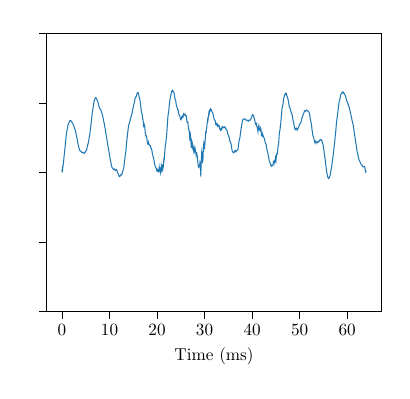
\begin{tikzpicture}[scale=0.62]

\definecolor{darkgray176}{RGB}{176,176,176}
\definecolor{steelblue31119180}{RGB}{31,119,180}

\begin{axis}[
yticklabel={\empty},
tick align=outside,
tick pos=left,
x grid style={darkgray176},
xlabel={Time (ms)},
xmin=-3.2, xmax=67.2,
xtick style={color=black},
y grid style={darkgray176},
% ylabel={Amplitude},
% ymin=-0.15, ymax=0.15,
ymin=-0.1, ymax=0.1,
ytick style={color=black}
]
\addplot [semithick, steelblue31119180]
table {%
0 0
0.0625610948191593 0.00267421979664707
0.125122189638319 0.00195263445792485
0.187683284457478 0.00448575329658223
0.250244379276637 0.00506307051416017
0.312805474095797 0.00741872769886972
0.375366568914956 0.00896099196129705
0.437927663734115 0.0115803680341702
0.500488758553275 0.0133900876509304
0.563049853372434 0.0151754755341063
0.625610948191593 0.0175304286389494
0.688172043010753 0.0195827149455586
0.750733137829912 0.0220035516719752
0.813294232649071 0.0241572310672827
0.875855327468231 0.0260075675241671
0.93841642228739 0.0276190532682753
1.00097751710655 0.029011056083869
1.06353861192571 0.0303319803605681
1.12609970674487 0.0314772311226626
1.18866080156403 0.0323503866813574
1.25122189638319 0.0340090383259345
1.31378299120235 0.0342868589673224
1.37634408602151 0.034962264941104
1.43890518084066 0.0355454103753539
1.50146627565982 0.0360117456070052
1.56402737047898 0.0365307936963797
1.62658846529814 0.0370469956639663
1.6891495601173 0.0372855405697375
1.75171065493646 0.0373638160362883
1.81427174975562 0.0371841114243804
1.87683284457478 0.0371509336557818
1.93939393939394 0.0367688526484099
2.0019550342131 0.0364753106155616
2.06451612903226 0.0361838696464416
2.12707722385142 0.0359691435804378
2.18963831867058 0.0355138606187011
2.25219941348974 0.0352915312351981
2.3147605083089 0.0347998261102134
2.37732160312805 0.0344101194336005
2.43988269794721 0.0336631536920749
2.50244379276637 0.0331262272681571
2.56500488758553 0.0324098647864333
2.62756598240469 0.0318902237095004
2.69012707722385 0.0313611501975318
2.75268817204301 0.030779401080743
2.81524926686217 0.0301372612829257
2.87781036168133 0.0291732079745475
2.94037145650049 0.0278471793837386
3.00293255131965 0.026998937900159
3.06549364613881 0.0261555616457092
3.12805474095797 0.0251639858926059
3.19061583577713 0.0240808387786762
3.25317693059629 0.0226956488526374
3.31573802541544 0.0215881998074457
3.3782991202346 0.0205637725818454
3.44086021505376 0.0194245896512462
3.50342130987292 0.0185915641158907
3.56598240469208 0.0176511272853595
3.62854349951124 0.016837186412203
3.6911045943304 0.0160462343054783
3.75366568914956 0.0156823699676658
3.81622678396872 0.0154439510553638
3.87878787878788 0.0154666042124683
3.94134897360704 0.0152564826052734
4.0039100684262 0.0150434925245487
4.06647116324536 0.01496300729445
4.12903225806452 0.0145273268102638
4.19159335288368 0.0143023412947781
4.25415444770283 0.0141885221670887
4.31671554252199 0.0143579145090496
4.37927663734115 0.0143627272509148
4.44183773216031 0.0143107777445023
4.50439882697947 0.0143003093455631
4.56695992179863 0.0140994674365017
4.62952101661779 0.0139923333422529
4.69208211143695 0.0136977836183788
4.75464320625611 0.013858715826072
4.81720430107527 0.0140708540115626
4.87976539589443 0.0146523808071778
4.94232649071359 0.0149836221114456
5.00488758553275 0.0151687482169821
5.06744868035191 0.0155991362598984
5.13000977517107 0.0159412591371281
5.19257086999022 0.0162529259035227
5.25513196480938 0.017360441337539
5.31769305962854 0.0182014699926999
5.3802541544477 0.0193291187581341
5.44281524926686 0.0200854901912625
5.50537634408602 0.0208316617795537
5.56793743890518 0.0217071624084914
5.63049853372434 0.0229126865049698
5.6930596285435 0.0242266035106175
5.75562072336266 0.0256323526474126
5.81818181818182 0.0267178274013779
5.88074291300098 0.0283921178146279
5.94330400782014 0.0298888944198659
6.0058651026393 0.0314556878562634
6.06842619745846 0.0335125506820042
6.13098729227761 0.0353603800185178
6.19354838709677 0.0371862264169801
6.25610948191593 0.0392754322130921
6.31867057673509 0.0411166230822938
6.38123167155425 0.0428521498174699
6.44379276637341 0.0441375720776246
6.50635386119257 0.0457053787929834
6.56891495601173 0.0472871441710904
6.63147605083089 0.048761960190019
6.69403714565005 0.0498478819788201
6.75659824046921 0.050987220705211
6.81915933528837 0.0516526354504121
6.88172043010753 0.052490993072429
6.94428152492669 0.0530063456738275
7.00684261974585 0.0534649434775289
7.069403714565 0.0537074036634038
7.13196480938416 0.0537072170656885
7.19452590420332 0.0535349667596677
7.25708699902248 0.0530148078673833
7.31964809384164 0.0528068320274003
7.3822091886608 0.0521574912434362
7.44477028347996 0.0515556330096162
7.50733137829912 0.0511457352595857
7.56989247311828 0.0503554332160181
7.63245356793744 0.0496244228928407
7.6950146627566 0.0487227421199297
7.75757575757576 0.0479266882281412
7.82013685239492 0.0471831423031095
7.88269794721408 0.046654381715526
7.94525904203324 0.0460351152001413
8.00782013685239 0.0457550140146898
8.07038123167155 0.0454348212550462
8.13294232649071 0.0452133226112798
8.19550342130987 0.0445972337685198
8.25806451612903 0.0439055550603136
8.32062561094819 0.0433501996252893
8.38318670576735 0.0427576806942476
8.44574780058651 0.0420135908768324
8.50830889540567 0.0413939108542246
8.57086999022483 0.040383708649629
8.63343108504399 0.0394220507029127
8.69599217986315 0.0382373149225439
8.75855327468231 0.0370243414417128
8.82111436950147 0.0361064742824549
8.88367546432062 0.0353182733026156
8.94623655913978 0.034049863776853
9.00879765395894 0.0328304045656122
9.0713587487781 0.0317752120300822
9.13391984359726 0.0303793267955965
9.19648093841642 0.0287503501471361
9.25904203323558 0.0277123870792364
9.32160312805474 0.0264058492072691
9.3841642228739 0.0252075347437624
9.44672531769306 0.0238300412674803
9.50928641251222 0.0225178186025176
9.57184750733138 0.0210519984932589
9.63440860215054 0.0198594470538439
9.6969696969697 0.0187120908363299
9.75953079178886 0.0173988586176962
9.82209188660802 0.0162397695983872
9.88465298142718 0.0150185930283188
9.94721407624633 0.0135728019423499
10.0097751710655 0.0123385272515921
10.0723362658847 0.0110240861762566
10.1348973607038 0.00961095098504398
10.197458455523 0.00825266510554073
10.2600195503421 0.0075971999443259
10.3225806451613 0.00651535481935547
10.3851417399804 0.00549221840684365
10.4477028347996 0.00441473745945787
10.5102639296188 0.00380801213386297
10.5728250244379 0.00333096788884782
10.6353861192571 0.0030224520516448
10.6979472140762 0.00274330640315485
10.7605083088954 0.00251342399357176
10.8230694037146 0.00208306508657695
10.8856304985337 0.00217947526630069
10.9481915933529 0.00227255503649761
11.010752688172 0.00244182444387867
11.0733137829912 0.00224105331533291
11.1358748778104 0.00175680994681599
11.1984359726295 0.00137892175367501
11.2609970674487 0.0013601645838218
11.3235581622678 0.001649708713779
11.386119257087 0.00193779625522951
11.4486803519062 0.00198972274349931
11.5112414467253 0.00166785174057631
11.5738025415445 0.00142994691833548
11.6363636363636 0.00061140903695063
11.6989247311828 -0.000307942650491191
11.761485826002 -0.000503915605132532
11.8240469208211 -0.00113124737401337
11.8866080156403 -0.00155196709236092
11.9491691104594 -0.00214502619049591
12.0117302052786 -0.00279614021264213
12.0742913000978 -0.00304161296212429
12.1368523949169 -0.00297893156076282
12.1994134897361 -0.00285662688817447
12.2619745845552 -0.00236801814582865
12.3245356793744 -0.0021942504504122
12.3870967741935 -0.00160614665477507
12.4496578690127 -0.00156108215123502
12.5122189638319 -0.0018311939707512
12.574780058651 -0.00173706366869012
12.6373411534702 -0.000912511972519309
12.6999022482893 -0.000196902665836721
12.7624633431085 0.000736978850013351
12.8250244379277 0.00106108622335968
12.8875855327468 0.00214182240806542
12.950146627566 0.00270913908383713
13.0127077223851 0.00340024156829129
13.0752688172043 0.00556807706673299
13.1378299120235 0.00725564627725183
13.2003910068426 0.00904701511400187
13.2629521016618 0.0112418273021399
13.3255131964809 0.0124709883655621
13.3880742913001 0.0139866596431938
13.4506353861193 0.0154722398884398
13.5131964809384 0.0179199806613919
13.5757575757576 0.0204215760935437
13.6383186705767 0.0226809065843607
13.7008797653959 0.0248251628578583
13.7634408602151 0.0266148869789416
13.8260019550342 0.0284216282261082
13.8885630498534 0.0303372205931508
13.9511241446725 0.0320307074273087
14.0136852394917 0.0336226689249627
14.0762463343109 0.0342720239436871
14.13880742913 0.0349491323751351
14.2013685239492 0.0356921560931241
14.2639296187683 0.0364141654485394
14.3264907135875 0.0373742953598325
14.3890518084066 0.0380467732554394
14.4516129032258 0.0389382684182736
14.514173998045 0.039927060713123
14.5767350928641 0.0404909389459493
14.6392961876833 0.0411950073032872
14.7018572825024 0.0419001485442311
14.7644183773216 0.0429625525753781
14.8269794721408 0.0438603695558488
14.8895405669599 0.0452642597727849
14.9521016617791 0.0463684541105001
15.0146627565982 0.0474161693220002
15.0772238514174 0.0484258940230367
15.1397849462366 0.048982958699907
15.2023460410557 0.0497803344033506
15.2649071358749 0.051131768807594
15.327468230694 0.0521033428106839
15.3900293255132 0.0531876813511083
15.4525904203324 0.0538189128325307
15.5151515151515 0.0541310210458257
15.5777126099707 0.0543522023735158
15.6402737047898 0.0549303894463785
15.702834799609 0.0555825384328267
15.7653958944282 0.0564133933201826
15.8279569892473 0.056831538196533
15.8905180840665 0.0572587951329534
15.9530791788856 0.057280189141937
16.0156402737048 0.0573616571822736
16.0782013685239 0.056989228402065
16.1407624633431 0.0559466459741952
16.2033235581623 0.0549218033787267
16.2658846529814 0.0539930620970876
16.3284457478006 0.0531750289925382
16.3910068426197 0.0521099569871366
16.4535679374389 0.0510703175386026
16.5161290322581 0.0493302415575712
16.5786901270772 0.0474945895286424
16.6412512218964 0.0456468005039213
16.7038123167155 0.0437111058040274
16.7663734115347 0.0426618811835554
16.8289345063539 0.0419866980607908
16.891495601173 0.0413465699197348
16.9540566959922 0.0398208843953798
17.0166177908113 0.0385363369120443
17.0791788856305 0.0372270050723532
17.1417399804497 0.0345423184062117
17.2043010752688 0.032461166021324
17.266862170088 0.0347551361239813
17.3294232649071 0.0341661413175619
17.3919843597263 0.0338865765739134
17.4545454545455 0.0314861332828348
17.5171065493646 0.0286533663273295
17.5796676441838 0.0271085365361307
17.6422287390029 0.0262852582228411
17.7047898338221 0.0263691197621945
17.7673509286412 0.0262591917002219
17.8299120234604 0.0251460206091317
17.8924731182796 0.023419109804015
17.9550342130987 0.0213664465766848
18.0175953079179 0.0208063320833043
18.080156402737 0.0203971048855275
18.1427174975562 0.0208537711262091
18.2052785923754 0.0216071604644536
18.2678396871945 0.020109887729205
18.3304007820137 0.0199684586124686
18.3929618768328 0.0197349161051673
18.455522971652 0.0194785226671752
18.5180840664712 0.0194128193889807
18.5806451612903 0.0193844509701575
18.6432062561095 0.0188214922176341
18.7057673509286 0.0173547650001878
18.7683284457478 0.0172885383187064
18.830889540567 0.0166502374325417
18.8934506353861 0.0162434242228783
18.9560117302053 0.0150629650757722
19.0185728250244 0.013391328265459
19.0811339198436 0.0127082065490683
19.1436950146628 0.0115744774434661
19.2062561094819 0.0109363535085906
19.2688172043011 0.0104743799254779
19.3313782991202 0.00898958691272917
19.3939393939394 0.00790707682344046
19.4565004887586 0.0066469337168502
19.5190615835777 0.00564898771733657
19.5816226783969 0.0047800187185363
19.644183773216 0.00409872611968224
19.7067448680352 0.00366864474681465
19.7693059628544 0.00332232838895314
19.8318670576735 0.00288059430803197
19.8944281524927 0.00273982084238809
19.9569892473118 0.000845879196159301
20.019550342131 0.000760033273321092
20.0821114369501 0.00095205489120001
20.1446725317693 0.0019063416846599
20.2072336265885 0.00162790942926211
20.2697947214076 0.000875847490608168
20.3323558162268 0.000575767573286014
20.3949169110459 0.00160671152786251
20.4574780058651 0.00388647337332149
20.5200391006843 0.00233205468489453
20.5826001955034 0.00152916488540837
20.6451612903226 0.00328123563479993
20.7077223851417 0.00326864568303582
20.7702834799609 -0.00020999720325568
20.8328445747801 0.000763068778598764
20.8954056695992 0.00438050786442945
20.9579667644184 0.0029384327555332
21.0205278592375 0.000206796255760179
21.0830889540567 0.00278985447351359
21.1456500488759 0.00508365880075263
21.208211143695 0.00488976083280753
21.2707722385142 0.00338998097718811
21.3333333333333 0.00464094616472721
21.3958944281525 0.00786668587683582
21.4584555229717 0.0097706981789856
21.5210166177908 0.00937353533384038
21.58357771261 0.0119085969113884
21.6461388074291 0.0154543465107155
21.7086999022483 0.0183054468160238
21.7712609970674 0.0201115640770655
21.8338220918866 0.0206162288205977
21.8963831867058 0.0229037094675551
21.9589442815249 0.0247902948616886
22.0215053763441 0.0266693644826451
22.0840664711632 0.030081022257679
22.1466275659824 0.0328973525659867
22.2091886608016 0.0361175192438088
22.2717497556207 0.0395221697477913
22.3343108504399 0.041304173204731
22.396871945259 0.0427716355006104
22.4594330400782 0.0439727842436333
22.5219941348974 0.04629844911615
22.5845552297165 0.0490542658088494
22.6471163245357 0.0508796651724759
22.7096774193548 0.0520982259223538
22.772238514174 0.0532420461729737
22.8347996089932 0.0545685695609914
22.8973607038123 0.0551733477560044
22.9599217986315 0.0559879976305619
23.0224828934506 0.0578949249723702
23.0850439882698 0.0583804640755101
23.147605083089 0.0584930904439031
23.2101661779081 0.0588970233377648
23.2727272727273 0.0583844416859475
23.3352883675464 0.0586766382225972
23.3978494623656 0.0583387540593263
23.4604105571848 0.0581928974350701
23.5229716520039 0.0575271020438577
23.5855327468231 0.0569285704942742
23.6480938416422 0.0559307399787599
23.7106549364614 0.0543003477199861
23.7732160312805 0.0534002241184198
23.8357771260997 0.0520780251260377
23.8983382209189 0.0516900767864457
23.960899315738 0.0508313895888692
24.0234604105572 0.049175866521742
24.0860215053763 0.0479400197584783
24.1485826001955 0.0473373903895665
24.2111436950147 0.046511578878874
24.2737047898338 0.0462514713264543
24.336265884653 0.0451448697848054
24.3988269794721 0.0451817311991083
24.4613880742913 0.0443530065114023
24.5239491691105 0.0426578202784673
24.5865102639296 0.0416546216196329
24.6490713587488 0.0413088361156389
24.7116324535679 0.041108225174576
24.7741935483871 0.0408650341654016
24.8367546432063 0.0398515648812143
24.8993157380254 0.038847956440447
24.9618768328446 0.0380346358281252
25.0244379276637 0.0378304746854078
25.0869990224829 0.0382387661689188
25.1495601173021 0.0390100164114992
25.2121212121212 0.0399538556283171
25.2746823069404 0.040413034577305
25.3372434017595 0.0400065938966715
25.3998044965787 0.0394734188400843
25.4623655913978 0.0394740778832666
25.524926686217 0.0411028750513918
25.5874877810362 0.0420756560485384
25.6500488758553 0.0417780720757162
25.7126099706745 0.0412677814774324
25.7751710654936 0.041175230032057
25.8377321603128 0.0413646532599527
25.900293255132 0.0417800190697405
25.9628543499511 0.0412614583269941
26.0254154447703 0.0406542915544989
26.0879765395894 0.0408050164667742
26.1505376344086 0.0405792076621325
26.2130987292278 0.0390043036023543
26.2756598240469 0.0368666124866068
26.3382209188661 0.0360929401389315
26.4007820136852 0.0362097313818781
26.4633431085044 0.036331480986212
26.5259042033236 0.0345905183860896
26.5884652981427 0.031986461903168
26.6510263929619 0.031094742556515
26.713587487781 0.0309626471546214
26.7761485826002 0.0293936625811274
26.8387096774194 0.0263035376706431
26.9012707722385 0.0239715223744118
26.9638318670577 0.0245473122229674
27.0263929618768 0.026747274624943
27.088954056696 0.0248879576893933
27.1515151515152 0.0209304007955573
27.2140762463343 0.0176937769814408
27.2766373411535 0.0196157470454743
27.3391984359726 0.0221516430880492
27.4017595307918 0.0213706412317117
27.4643206256109 0.0188635372914527
27.5268817204301 0.0167689943505872
27.5894428152493 0.0163053760518077
27.6520039100684 0.0177176835621732
27.7145650048876 0.0165713070960076
27.7771260997067 0.0141103166617082
27.8396871945259 0.0146560471428454
27.9022482893451 0.0159809314031318
27.9648093841642 0.0179326702619403
28.0273704789834 0.0170464531690581
28.0899315738025 0.0151981798565982
28.1524926686217 0.0144559601349128
28.2150537634409 0.0127864169377473
28.27761485826 0.0140569939160627
28.3401759530792 0.0141271333486017
28.4027370478983 0.0123410444444488
28.4652981427175 0.0116867676508392
28.5278592375367 0.00907893372355493
28.5904203323558 0.00709933834013876
28.652981427175 0.00512608153816542
28.7155425219941 0.00378594341035113
28.7781036168133 0.00356751068050036
28.8406647116325 0.00437589089148555
28.9032258064516 0.00465376368693767
28.9657869012708 0.00537902522078357
29.0283479960899 0.00695361941506611
29.0909090909091 0.00594923797656189
29.1534701857282 0.0013902217881683
29.2160312805474 -0.00304396178496898
29.2785923753666 0.00566547975228154
29.3411534701857 0.0108653606896089
29.4037145650049 0.014694018147427
29.466275659824 0.0133876833037809
29.5288367546432 0.0101675867400736
29.5913978494624 0.00803752129356707
29.6539589442815 0.00901241266766776
29.7165200391007 0.0144135524133696
29.7790811339198 0.0189351138667015
29.841642228739 0.0207817511103195
29.9042033235582 0.0193139174816545
29.9667644183773 0.0165541066113543
30.0293255131965 0.0189539923051323
30.0918866080156 0.0218169781491379
30.1544477028348 0.0246398184022421
30.217008797654 0.0282433863696465
30.2795698924731 0.0278777189913296
30.3421309872923 0.0289339464911617
30.4046920821114 0.0309737586632065
30.4672531769306 0.0327821483513302
30.5298142717498 0.0346808726039013
30.5923753665689 0.0366036100777363
30.6549364613881 0.0380971568562855
30.7174975562072 0.0375351592286591
30.7800586510264 0.0395417567124028
30.8426197458456 0.0406106800015721
30.9051808406647 0.0431468461276936
30.9677419354839 0.0440592289932313
31.030303030303 0.0431223926557736
31.0928641251222 0.044251091953072
31.1554252199413 0.044091906240128
31.2179863147605 0.0447321454734921
31.2805474095797 0.0457030936278119
31.3431085043988 0.0453781697494893
31.405669599218 0.0451644942153496
31.4682306940371 0.0443997886414227
31.5307917888563 0.0437652633369756
31.5933528836755 0.0434029524452176
31.6559139784946 0.043035791225491
31.7184750733138 0.0426897188741441
31.7810361681329 0.0420002157354722
31.8435972629521 0.0409411973268056
31.9061583577713 0.039571873412148
31.9687194525904 0.0386384047371202
32.0312805474096 0.0383785877573438
32.0938416422287 0.0375490882092557
32.1564027370479 0.0375753101944661
32.2189638318671 0.0374420748537412
32.2815249266862 0.0360706945788388
32.3440860215054 0.0350615131037851
32.4066471163245 0.0339929430507932
32.4692082111437 0.0340246002345491
32.5317693059629 0.0349592938636842
32.594330400782 0.0352224107842641
32.6568914956012 0.034789714257607
32.7194525904203 0.0336865213565812
32.7820136852395 0.0331596681176305
32.8445747800587 0.0334299338702932
32.9071358748778 0.0338081808875471
32.969696969697 0.033365224911408
33.0322580645161 0.0329333330474554
33.0948191593353 0.0332109972266508
33.1573802541544 0.0320883396838155
33.2199413489736 0.0309007317046266
33.2825024437928 0.0308718603716131
33.3450635386119 0.030459921162499
33.4076246334311 0.0313069512603307
33.4701857282502 0.0315470496121565
33.5327468230694 0.0310009366223627
33.5953079178886 0.0306450518563696
33.6578690127077 0.0318058445295892
33.7204301075269 0.0329603675392366
33.782991202346 0.0327633887562147
33.8455522971652 0.032416258422423
33.9081133919844 0.0322558210119387
33.9706744868035 0.0320788991918837
34.0332355816227 0.0323125378903318
34.0957966764418 0.0326428515973154
34.158357771261 0.0326298984297472
34.2209188660802 0.032318359519467
34.2834799608993 0.0326219256421076
34.3460410557185 0.0323100589062811
34.4086021505376 0.0318218369277254
34.4711632453568 0.0310809285082251
34.533724340176 0.0310058263226076
34.5962854349951 0.0309875087370096
34.6588465298143 0.0306313110466315
34.7214076246334 0.0300611066044775
34.7839687194526 0.0293552047379118
34.8465298142717 0.0284407946480509
34.9090909090909 0.0275458454747092
34.9716520039101 0.0268777255023505
35.0342130987292 0.0267992109508196
35.0967741935484 0.0259139400816733
35.1593352883675 0.0252057173592516
35.2218963831867 0.0244404716182314
35.2844574780059 0.0227533189738251
35.347018572825 0.0225678494751803
35.4095796676442 0.0221244483268506
35.4721407624633 0.0217717170190951
35.5347018572825 0.0210364933925902
35.5972629521017 0.0201191887521674
35.6598240469208 0.0188929513752286
35.72238514174 0.0170571037685591
35.7849462365591 0.0159716786396119
35.8475073313783 0.0150278387563931
35.9100684261975 0.01489631146127
35.9726295210166 0.0146592597305076
36.0351906158358 0.0141087751125485
36.0977517106549 0.014124936951308
36.1603128054741 0.014254863567847
36.2228739002933 0.0143559359483792
36.2854349951124 0.0151110854862897
36.3479960899316 0.0150740762566192
36.4105571847507 0.0157257782082316
36.4731182795699 0.0156458070681941
36.5356793743891 0.0150090577654388
36.5982404692082 0.0147384244052808
36.6608015640274 0.015120394850188
36.7233626588465 0.0154524166027734
36.7859237536657 0.0158782299892032
36.8484848484849 0.0158998847685077
36.911045943304 0.0161424008337371
36.9736070381232 0.0162015636984117
37.0361681329423 0.0167102424422405
37.0987292277615 0.0182204747960365
37.1612903225806 0.0200580241939714
37.2238514173998 0.0217561341133897
37.286412512219 0.0231641612652023
37.3489736070381 0.0238318093219373
37.4115347018573 0.0247525442883241
37.4740957966764 0.025644510700381
37.5366568914956 0.0275202778514879
37.5992179863148 0.0292770331534298
37.6617790811339 0.0308391401746318
37.7243401759531 0.0322980790063083
37.7869012707722 0.0334602463116482
37.8494623655914 0.0347619480904072
37.9120234604106 0.0359631676139457
37.9745845552297 0.0368996791847465
38.0371456500489 0.0378674757434738
38.099706744868 0.0381146148939636
38.1622678396872 0.0383059976245563
38.2248289345064 0.0384774612279232
38.2873900293255 0.0383171840049217
38.3499511241447 0.0384484256489361
38.4125122189638 0.0384597241212109
38.475073313783 0.0384790841216915
38.5376344086022 0.0383175552011498
38.6001955034213 0.0377998699016235
38.6627565982405 0.0377321959448612
38.7253176930596 0.0376487938124588
38.7878787878788 0.0376734474504536
38.8504398826979 0.0375150216967304
38.9130009775171 0.0375846544897888
38.9755620723363 0.0374904452902306
39.0381231671554 0.0374442960608128
39.1006842619746 0.0372936971420067
39.1632453567937 0.0369457174420269
39.2258064516129 0.0368236430710362
39.2883675464321 0.0373380606245697
39.3509286412512 0.0374558800476387
39.4134897360704 0.0376636466049641
39.4760508308895 0.0376178475528344
39.5386119257087 0.0375941767250775
39.6011730205279 0.0375067810814751
39.663734115347 0.0377316429959801
39.7262952101662 0.0381126951568287
39.7888563049853 0.0388838746188935
39.8514173998045 0.0394202564840268
39.9139784946237 0.0397456081043328
39.9765395894428 0.040315290339444
40.039100684262 0.0412298003457421
40.1016617790811 0.0414068146316537
40.1642228739003 0.0410492199574136
40.2267839687195 0.0411880649189271
40.2893450635386 0.0409462820694856
40.3519061583578 0.0401449904195374
40.4144672531769 0.0390465733406743
40.4770283479961 0.0386799932662343
40.5395894428152 0.0376865399668206
40.6021505376344 0.0366314517394189
40.6647116324536 0.0358175872347135
40.7272727272727 0.0348084318366918
40.7898338220919 0.0344157486531304
40.852394916911 0.0347675312081041
40.9149560117302 0.0350688882335977
40.9775171065494 0.0333061736634225
41.0400782013685 0.032600074356471
41.1026392961877 0.0321379145088434
41.1652003910068 0.0307046050080194
41.227761485826 0.0294969624176053
41.2903225806452 0.0325823667188806
41.3528836754643 0.0329074016895112
41.4154447702835 0.0337845209570836
41.4780058651026 0.0325840122975912
41.5405669599218 0.0306703675909738
41.603128054741 0.0305694714953298
41.6656891495601 0.030171353113223
41.7282502443793 0.031143564140954
41.7908113391984 0.0318894302554407
41.8533724340176 0.0306748176468782
41.9159335288368 0.0292985609669752
41.9784946236559 0.0267994198347292
42.0410557184751 0.0260753441394424
42.1036168132942 0.026039359364604
42.1661779081134 0.0267842792553549
42.2287390029325 0.0277295210439701
42.2913000977517 0.0265493077660236
42.3538611925709 0.0261299217016029
42.41642228739 0.0255084721661034
42.4789833822092 0.0248335181486921
42.5415444770283 0.0245418480742187
42.6041055718475 0.0241732470297918
42.6666666666667 0.0232807192951441
42.7292277614858 0.0216111164933338
42.791788856305 0.0214149535488873
42.8543499511241 0.0207516336130781
42.9169110459433 0.0204178342306194
42.9794721407625 0.0192357806592655
43.0420332355816 0.0175879018878307
43.1045943304008 0.0168795692693453
43.1671554252199 0.0155753857808466
43.2297165200391 0.0148914705776224
43.2922776148583 0.0144289083986426
43.3548387096774 0.0130980704580584
43.4173998044966 0.0120939013611012
43.4799608993157 0.0108472363548108
43.5425219941349 0.00960976536497692
43.6050830889541 0.00849363266809944
43.6676441837732 0.00765429090304284
43.7302052785924 0.00705099843245797
43.7927663734115 0.00663502100866037
43.8553274682307 0.00606322959283929
43.9178885630498 0.00568777587690836
43.980449657869 0.00445893265940576
44.0430107526882 0.00439443637526804
44.1055718475073 0.00446561516380031
44.1681329423265 0.00513564554368121
44.2306940371457 0.00521406070861823
44.2932551319648 0.00499794883462341
44.355816226784 0.00488837840051945
44.4183773216031 0.00564268229753216
44.4809384164223 0.00737928005366906
44.5434995112414 0.00707713632552155
44.6060606060606 0.0070919179442254
44.6686217008798 0.00851020454551992
44.7311827956989 0.00866406987751684
44.7937438905181 0.00704828820729361
44.8563049853372 0.00816068935953627
44.9188660801564 0.0108787558229962
44.9814271749756 0.010371167922824
45.0439882697947 0.00914865583618366
45.1065493646139 0.0114646889706336
45.169110459433 0.0132357996787406
45.2316715542522 0.0134156004817954
45.2942326490714 0.0132334446288711
45.3567937438905 0.0144499974472781
45.4193548387097 0.0173056817222987
45.4819159335288 0.019130442198639
45.544477028348 0.0196244097710792
45.6070381231672 0.021854941905244
45.6695992179863 0.025132772351596
45.7321603128055 0.0278786127168762
45.7947214076246 0.0295117591614248
45.8572825024438 0.0303778906852619
45.919843597263 0.0322564648426086
45.9824046920821 0.0339553831500217
46.0449657869013 0.0358612972128688
46.1075268817204 0.0385077691847278
46.1700879765396 0.0408807266175834
46.2326490713588 0.0432648152178508
46.2952101661779 0.0456662636709091
46.3577712609971 0.046847217615224
46.4203323558162 0.0477867429458763
46.4828934506354 0.0485950412004749
46.5454545454545 0.0505165232514793
46.6080156402737 0.0525513137322018
46.6705767350929 0.0537294811593735
46.733137829912 0.0543446789913513
46.7956989247312 0.0549502618490688
46.8582600195503 0.0558704715495235
46.9208211143695 0.0559133530329487
46.9833822091887 0.0559761648194706
47.0459433040078 0.0569916450940182
47.108504398827 0.0570250419883434
47.1710654936461 0.0568927230690319
47.2336265884653 0.056640900562236
47.2961876832845 0.0551848630653011
47.3587487781036 0.0547586485437634
47.4213098729228 0.0541026841936486
47.4838709677419 0.0536307193819554
47.5464320625611 0.0527246055135891
47.6089931573803 0.0517289356664479
47.6715542521994 0.0508142424545243
47.7341153470186 0.0493116723564713
47.7966764418377 0.0481130375179989
47.8592375366569 0.0468085671821473
47.9217986314761 0.0465829856202137
47.9843597262952 0.0462157163670685
48.0469208211144 0.0452095076736729
48.1094819159335 0.0442796264532025
48.1720430107527 0.0438324161955426
48.2346041055718 0.0430557673409188
48.297165200391 0.0426278280099728
48.3597262952102 0.0418391911711686
48.4222873900293 0.041594998058904
48.4848484848485 0.0406052067198537
48.5474095796676 0.0389845076664365
48.6099706744868 0.0375579707433751
48.672531769306 0.0365544479842847
48.7350928641251 0.0357116901280244
48.7976539589443 0.0348651324756596
48.8602150537634 0.0336367660953153
48.9227761485826 0.0324083252091649
48.9853372434018 0.0313928293670552
49.0478983382209 0.0309147811563046
49.1104594330401 0.030692954686992
49.1730205278592 0.0309709876699269
49.2355816226784 0.031597696648927
49.2981427174976 0.0318774469906896
49.3607038123167 0.0314093900085195
49.4232649071359 0.0308339031047223
49.485826001955 0.0304353637648118
49.5483870967742 0.031060064812341
49.6109481915934 0.0315283893490117
49.6735092864125 0.031664160946029
49.7360703812317 0.0318912170565198
49.7986314760508 0.0325307298582757
49.86119257087 0.0333566375601152
49.9237536656891 0.0340274055474752
49.9863147605083 0.0343475082337507
50.0488758553275 0.0348904801374219
50.1114369501466 0.0352367120098508
50.1739980449658 0.0354705928521684
50.2365591397849 0.0357889670037454
50.2991202346041 0.0362658038287481
50.3616813294233 0.0370228979681944
50.4242424242424 0.0380117535929788
50.4868035190616 0.0389377374933962
50.5493646138807 0.0395894841484922
50.6119257086999 0.0399620687244924
50.6744868035191 0.0408489817802595
50.7370478983382 0.0415870843897642
50.7996089931574 0.0421664896325544
50.8621700879765 0.0424486465118498
50.9247311827957 0.04317258929293
50.9872922776149 0.0436714500341772
51.049853372434 0.0439890157977594
51.1124144672532 0.044358433877006
51.1749755620723 0.0441271898738188
51.2375366568915 0.0438700103995737
51.3000977517107 0.0442643841985296
51.3626588465298 0.0446783232221331
51.425219941349 0.0449076517597059
51.4877810361681 0.0448242272755617
51.5503421309873 0.0448317967322477
51.6129032258064 0.0444544803711676
51.6754643206256 0.0442608096459307
51.7380254154448 0.0440060031816057
51.8005865102639 0.0440069565227217
51.8631476050831 0.0439781410690626
51.9257086999022 0.0437708097043013
51.9882697947214 0.0431585281082262
52.0508308895406 0.0425149987771277
52.1133919843597 0.0415439978023428
52.1759530791789 0.0401725728239569
52.238514173998 0.0387360111447024
52.3010752688172 0.0377038967825713
52.3636363636364 0.0366723598404364
52.4261974584555 0.0354431589950652
52.4887585532747 0.0341393890137896
52.5513196480938 0.0325012071730017
52.613880742913 0.0306788693315997
52.6764418377322 0.0291148989988475
52.7390029325513 0.0275694079686208
52.8015640273705 0.0265256427610812
52.8641251221896 0.0256399043680024
52.9266862170088 0.0253011354482856
52.989247311828 0.0243811560494284
53.0518084066471 0.0233437759894605
53.1143695014663 0.0225893578046927
53.1769305962854 0.0217172744632029
53.2394916911046 0.0211648024028697
53.3020527859238 0.0224554698717647
53.3646138807429 0.0222937956649013
53.4271749755621 0.0224200454199157
53.4897360703812 0.0216772929817176
53.5522971652004 0.0212178265189757
53.6148582600196 0.0211791725736385
53.6774193548387 0.0211344315039535
53.7399804496579 0.0214040229790721
53.802541544477 0.0220809991627145
53.8651026392962 0.0223197899376455
53.9276637341153 0.0223311759542423
53.9902248289345 0.0219567615943046
54.0527859237537 0.0220094107888923
54.1153470185728 0.0223439676015258
54.177908113392 0.0227976033185497
54.2404692082111 0.0232850162427097
54.3030303030303 0.0231732385741039
54.3655913978495 0.0234766053937135
54.4281524926686 0.0236280772266937
54.4907135874878 0.0235211834136692
54.5532746823069 0.0233881529639106
54.6158357771261 0.0231276766077514
54.6783968719453 0.0227126081547867
54.7409579667644 0.0217724376825119
54.8035190615836 0.0213462827656189
54.8660801564027 0.0205169620314651
54.9286412512219 0.020012508963079
54.9912023460411 0.0188231631359659
55.0537634408602 0.0171258385863996
55.1163245356794 0.0157880976828924
55.1788856304985 0.0139106013306862
55.2414467253177 0.0122885611727615
55.3040078201369 0.0112943628152882
55.366568914956 0.0093972099688221
55.4291300097752 0.00770373364413414
55.4916911045943 0.00584246838175831
55.5542521994135 0.00412534391425572
55.6168132942326 0.00245839351913796
55.6793743890518 0.000780038147771465
55.741935483871 -0.000622202431963335
55.8044965786901 -0.00163171173256339
55.8670576735093 -0.00270341847998656
55.9296187683284 -0.00340635501547468
55.9921798631476 -0.00384208765372503
56.0547409579668 -0.00413895264551961
56.1173020527859 -0.00444098088966786
56.1798631476051 -0.00418070636558568
56.2424242424242 -0.00360199775208126
56.3049853372434 -0.00304885953118549
56.3675464320626 -0.00252012568703495
56.4301075268817 -0.0017775341027206
56.4926686217009 -0.000825290630989413
56.55522971652 0.000563787831720022
56.6177908113392 0.00183773806040063
56.6803519061584 0.00313017317954221
56.7429130009775 0.00412363140049044
56.8054740957967 0.00566291729332415
56.8680351906158 0.00711228026628844
56.930596285435 0.0089067299181153
56.9931573802542 0.0104306080102746
57.0557184750733 0.0119805407827813
57.1182795698925 0.0143055500042054
57.1808406647116 0.0158458994674193
57.2434017595308 0.0175163397931458
57.3059628543499 0.0196888505309121
57.3685239491691 0.0215753390674979
57.4310850439883 0.023990589721112
57.4936461388074 0.0260414846317946
57.5562072336266 0.0279752023987844
57.6187683284457 0.0300400056807963
57.6813294232649 0.03277259705113
57.7438905180841 0.0352639255832193
57.8064516129032 0.0372064629749906
57.8690127077224 0.0387646770678308
57.9315738025415 0.0404650743154924
57.9941348973607 0.0420708640907342
58.0566959921799 0.0439263153711984
58.119257086999 0.0457073502526605
58.1818181818182 0.0474987526170232
58.2443792766373 0.0490374536392801
58.3069403714565 0.0505239223662622
58.3695014662757 0.0515297504136464
58.4320625610948 0.0522976404443777
58.494623655914 0.0528898979386976
58.5571847507331 0.0540614753273313
58.6197458455523 0.0552708644124944
58.6823069403715 0.0560077898302648
58.7448680351906 0.0564124975845087
58.8074291300098 0.0568147131195428
58.8699902248289 0.0571315971550005
58.9325513196481 0.0569640071871431
58.9951124144673 0.0570515101977632
59.0576735092864 0.0578324908986032
59.1202346041056 0.0576970315595701
59.1827956989247 0.057722884741041
59.2453567937439 0.0576931007119043
59.307917888563 0.0567069899596689
59.3704789833822 0.0566763006849897
59.4330400782014 0.05626079637306
59.4956011730205 0.0559517869348925
59.5581622678397 0.0556505410017069
59.6207233626588 0.055134919513006
59.683284457478 0.0544264769984568
59.7458455522972 0.053288635172365
59.8084066471163 0.0526271909202211
59.8709677419355 0.0517917160064943
59.9335288367546 0.0514830865479372
59.9960899315738 0.051134827451185
60.058651026393 0.0505215214002779
60.1212121212121 0.0497802963311022
60.1837732160313 0.0491487996876677
60.2463343108504 0.0484007759636973
60.3088954056696 0.0478875684631098
60.3714565004888 0.0473363406497362
60.4340175953079 0.0468872565710562
60.4965786901271 0.0460121147662314
60.5591397849462 0.0450108979618357
60.6217008797654 0.0438298725706042
60.6842619745846 0.0428822552430228
60.7468230694037 0.0419466333502024
60.8093841642229 0.0411196371971949
60.871945259042 0.0403209532504557
60.9345063538612 0.039276586408533
60.9970674486804 0.0380582447843817
61.0596285434995 0.0371007740639609
61.1221896383187 0.0360698294429835
61.1847507331378 0.0353156627153109
61.247311827957 0.0343963464181269
61.3098729227762 0.0335445323811511
61.3724340175953 0.031944404380762
61.4349951124145 0.0303682355849274
61.4975562072336 0.0286385904167317
61.5601173020528 0.0272719170461215
61.6226783968719 0.0258196607188395
61.6852394916911 0.0243035696796483
61.7478005865103 0.0227989208696088
61.8103616813294 0.021500640103588
61.8729227761486 0.0203646199444522
61.9354838709677 0.0187503377035741
61.9980449657869 0.0170625145069141
62.0606060606061 0.0159145622429523
62.1231671554252 0.0145981244120168
62.1857282502444 0.0137994386026324
62.2482893450635 0.012727528826888
62.3108504398827 0.0117746551146955
62.3734115347019 0.0107542865928754
62.435972629521 0.00994687242832177
62.4985337243402 0.00900293568755525
62.5610948191593 0.00859378858351987
62.6236559139785 0.00813819083475298
62.6862170087977 0.00771863340697855
62.7487781036168 0.00717838961205
62.811339198436 0.00671188235064406
62.8739002932551 0.00621034618456168
62.9364613880743 0.00593350649076647
62.9990224828935 0.0054801793064365
63.0615835777126 0.00537889578060146
63.1241446725318 0.00507545192613979
63.1867057673509 0.0048174845529966
63.2492668621701 0.00437471670401761
63.3118279569892 0.00417060399007413
63.3743890518084 0.00395582949529645
63.4369501466276 0.00400284605095289
63.4995112414467 0.00400681501456544
63.5620723362659 0.00419773767180632
63.624633431085 0.00398296317702864
63.6871945259042 0.00392700898354529
63.7497556207234 0.0032044941848936
63.8123167155425 0.00166316802922057
63.8748778103617 0.000470869909545896
63.9374389051808 0.000761237328659056
64 0
};
\end{axis}

\end{tikzpicture}

	\end{subfigure}\hfill
	\begin{subfigure}{0.3\textwidth}
		\centering
		% This file was created with tikzplotlib v0.10.1.
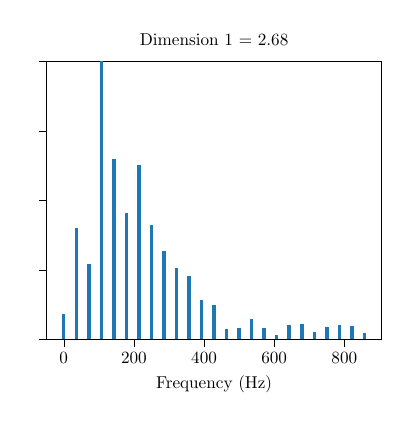
\begin{tikzpicture}[scale=0.62]

\definecolor{darkgray176}{RGB}{176,176,176}
\definecolor{steelblue31119180}{RGB}{31,119,180}

\begin{axis}[
yticklabel={\empty},
tick align=outside,
tick pos=left,
x grid style={darkgray176},
xlabel={Frequency (Hz)},
xmin=-48.3571428571429, xmax=905.5,
xtick style={color=black},
y grid style={darkgray176},
%ylabel={Magnitude},
ymin=0, ymax=4,
title={Dimension 1 = 2.68},
ytick style={color=black}
]
\draw[draw=none,fill=steelblue31119180] (axis cs:-5,0) rectangle (axis cs:5,0.363293109461665);
\draw[draw=none,fill=steelblue31119180] (axis cs:30.7142857142857,0) rectangle (axis cs:40.7142857142857,1.59671692845371);
\draw[draw=none,fill=steelblue31119180] (axis cs:66.4285714285714,0) rectangle (axis cs:76.4285714285714,1.08375129075336);
\draw[draw=none,fill=steelblue31119180] (axis cs:102.142857142857,0) rectangle (axis cs:112.142857142857,5.72028640718505);
\draw[draw=none,fill=steelblue31119180] (axis cs:137.857142857143,0) rectangle (axis cs:147.857142857143,2.60109171070077);
\draw[draw=none,fill=steelblue31119180] (axis cs:173.571428571429,0) rectangle (axis cs:183.571428571429,1.82230187959835);
\draw[draw=none,fill=steelblue31119180] (axis cs:209.285714285714,0) rectangle (axis cs:219.285714285714,2.50466396839656);
\draw[draw=none,fill=steelblue31119180] (axis cs:245,0) rectangle (axis cs:255,1.64154431128106);
\draw[draw=none,fill=steelblue31119180] (axis cs:280.714285714286,0) rectangle (axis cs:290.714285714286,1.2779936763853);
\draw[draw=none,fill=steelblue31119180] (axis cs:316.428571428571,0) rectangle (axis cs:326.428571428571,1.02566988726104);
\draw[draw=none,fill=steelblue31119180] (axis cs:352.142857142857,0) rectangle (axis cs:362.142857142857,0.906444113984638);
\draw[draw=none,fill=steelblue31119180] (axis cs:387.857142857143,0) rectangle (axis cs:397.857142857143,0.567573738688084);
\draw[draw=none,fill=steelblue31119180] (axis cs:423.571428571429,0) rectangle (axis cs:433.571428571429,0.497884322563813);
\draw[draw=none,fill=steelblue31119180] (axis cs:459.285714285714,0) rectangle (axis cs:469.285714285714,0.143370970638671);
\draw[draw=none,fill=steelblue31119180] (axis cs:495,0) rectangle (axis cs:505,0.158030205491621);
\draw[draw=none,fill=steelblue31119180] (axis cs:530.714285714286,0) rectangle (axis cs:540.714285714286,0.287791882784369);
\draw[draw=none,fill=steelblue31119180] (axis cs:566.428571428571,0) rectangle (axis cs:576.428571428571,0.164560600100172);
\draw[draw=none,fill=steelblue31119180] (axis cs:602.142857142857,0) rectangle (axis cs:612.142857142857,0.0653538748355305);
\draw[draw=none,fill=steelblue31119180] (axis cs:637.857142857143,0) rectangle (axis cs:647.857142857143,0.209706204538538);
\draw[draw=none,fill=steelblue31119180] (axis cs:673.571428571429,0) rectangle (axis cs:683.571428571429,0.216581742305538);
\draw[draw=none,fill=steelblue31119180] (axis cs:709.285714285714,0) rectangle (axis cs:719.285714285714,0.104565114650486);
\draw[draw=none,fill=steelblue31119180] (axis cs:745,0) rectangle (axis cs:755,0.18370350932939);
\draw[draw=none,fill=steelblue31119180] (axis cs:780.714285714286,0) rectangle (axis cs:790.714285714286,0.206670350113575);
\draw[draw=none,fill=steelblue31119180] (axis cs:816.428571428571,0) rectangle (axis cs:826.428571428571,0.196489132073225);
\draw[draw=none,fill=steelblue31119180] (axis cs:852.142857142857,0) rectangle (axis cs:862.142857142857,0.0885177801919891);
\end{axis}

\end{tikzpicture}

	\end{subfigure}
	
	\caption{The twelfth dimension is being modified, while other dimensions are fixed at 0. Negative values cause a large spike around 100Hz while positive values fully remove the 100Hz and influences the 150Hz range instead.}
	\label{fig:interpol_dim12}
\end{figure}
